\def\coursename{概率论}
\def\coursefullname{概率论、数理统计和随机过程初步}
\def\courseEnglishname{Probability and Statistics}
\def\teachername{唐宏岩老师、续本达}
\def\beginday{2022/9/13}


\documentclass[a4paper, 11pt]{article}

\usepackage[UTF8]{ctex}

\usepackage[T1]{fontenc}								% 字体
\catcode`\。=\active
\newcommand{。}{.} % {\ifmmode\text{.}\else .\fi}
\catcode`\(=\active
\catcode`\)=\active
\newcommand{(}{(}
\newcommand{)}{)}

% \usepackage{zhlineskip}

\usepackage{nicematrix}
% \usepackage{setspace}
% \linespread{1}						% 一倍行距
\setlength{\headheight}{14pt}			% 页眉高度
% \setlength{\lineskip}{0ex}			% 行距
\renewcommand\arraystretch{.82}		% 表格

\usepackage{amssymb, amsmath, amsfonts, amsthm}			% 数学符号,公式,字体,定理环境
\everymath{\displaystyle}			% \textstyle \scriptstyle \scriptscriptstyle
\allowdisplaybreaks[4]      		% 使用行间公式格式
% \makeatletter
% \renewcommand{\maketag@@@}[1]{\hbox{\m@th\normalsize\normalfont#1}}
% \makeatother
\newif\ifcontent\contenttrue		% if 显示目录
\newif\ifparskip\parskipfalse		% if 增加目录后的行距
\newif\ifshowemail\showemailfalse	% if 显示 email
\def\firstandforemost{
	\maketitle
	%\thispagestyle{empty}\clearpage
	\ifcontent
		\renewcommand{\contentsname}{目录}
		\tableofcontents
		\thispagestyle{empty}
		\clearpage
	\fi
	\ifparskip
		\setlength{\parskip}{.8ex}	% 设置额外的段距,目录后
	\fi								% 在 \firstandforemost 前设置 \parskiptrue
	\makenomenclature
	\printnomenclature
	\setcounter{page}{1}
}

\usepackage{mathtools}									% \rcase 环境等

% \usepackage{physics}

\usepackage[]{siunitx}									% 国际制单位
\sisetup{
	inter-unit-product = \ensuremath{{}\cdot{}},
	per-mode = symbol,
	per-mode = reciprocal-positive-first,
	range-units = single,
	separate-uncertainty = true,
	range-phrase = \ifmmode\text{\;-\;}\else\;-\;\fi
}
\DeclareSIUnit\angstrom{\text{Å}}
\DeclareSIUnit\atm{\text{atm}}
% SIunits 额外定义了一个 \square 表示平方,
% 还会把 \cdot 空格加大,真有够无语的 😅

\usepackage{authblk}									% 作者介绍
\ifx \coursefullname\undefined
	\ifx \coursename\undefined
		\def\coursename{笔记}
	\fi
	\def\coursefullname{\coursename}
\fi
\ifx \authorname\undefined
	\def\authorname{Dait}
\fi
\ifx \departmentname\undefined
	\def\departmentname{DEP 00, THU}
\fi
\ifx \emailaddress\undefined
	\def\emailaddress{daiyj20@mails.tsinghua.edu.cn}
\fi
\ifx \beginday\undefined
	\def\beginday{2021}
\fi
\ifx \endday\undefined
	\def\endday{\number\year/\number\month/\number\day}
\fi
\ifx \titleannotation\undefined
	\ifx \teachername\undefined
		\title{\textbf{\coursefullname}}
	\else
		\title{\textbf{\coursefullname}\\\small\textit{主要整理自\teachername 老师讲义}}
	\fi
\else
	\title{\textbf{\coursefullname}\\\small\textit{(\titleannotation)}}
\fi
\newif\ifdefaultauthor\defaultauthortrue
\ifdefaultauthor
	\author{by~\authorname~at~\departmentname}
	\ifshowemail
		\affil{\emailaddress}
	\fi
\fi
\ifx \endday\beginday
	\date{\beginday}
\else
	\date{\beginday~-~\endday}
\fi

\usepackage{hyperref}									% 链接
\ifx \courseEnglishname\undefined
	\def\courseEnglishname{Note}
\fi
\ifx \authorEnglishname\undefined
	\def\authorEnglishname{Dait}
\fi
\hypersetup{
	% dvipdfm								% 表示用 dvipdfm 生成 pdf
	pdftitle={\coursename},
	pdfauthor={\authorname},
	colorlinks=true, breaklinks=true,		% 超链接设置
	linkcolor=black, citecolor=black, urlcolor=blue
}

\usepackage[british]{babel}								% 长单词自动连字符换行
\hyphenation{long-sen-ten-ce}				% 自定义拆分方式

\usepackage{tikz}
\usetikzlibrary{quotes, angles}
\usepackage{pgfplots}
\pgfplotsset{compat=1.17}								% TikZ
\newcommand{\coor}[5][0]{
	\draw[thick,latex-latex](#1,#3)node[left]{$#5$}--(#1,0)node[shift={(-135:7pt)}]{$O$}--(#1+#2,0)node[right]{$#4$}
}			% 坐标轴

\usepackage{enumerate}									% 编号
\usepackage{paralist}
\setlength{\pltopsep}{1ex}
\setlength{\plitemsep}{1ex}
\ifx \eqnrange\undefined
	\numberwithin{equation}{section}
\else
	\numberwithin{equation}{\eqnrange}
\fi

\renewcommand{\thempfootnote}{\Roman{mpfootnote}}
\renewcommand{\thefootnote}{\Roman{footnote}}		% 注释上标 I, II,...
\newcommand{\sectionstar}[1]{
	\section[\hspace{-.8em}*\hspace{.3em}#1]{\hspace{-1em}*\hspace{.5em}#1}
}
\newcommand{\subsectionstar}[1]{					% 带星号的 section 和 subsection
	\subsection{\hspace{-1em}*\hspace{.5em}#1}
}
\newcommand{\subsubsectionstar}[1]{					% 带星号的 section 和 subsection
	\subsubsection{\hspace{-1em}*\hspace{.5em}#1}
}
\newcommand*{\appendiks}{
	\appendix
	\part*{附录}
	\addcontentsline{toc}{part}{附录}
}
\iffalse			% 不清楚
	\newcommand{\varsection}[1]{
		\refstepcounter{section}
		\section*{\thesection\quad #1}
		\addcontentsline{toc}{section}{\makebox[0pt][r]{*}\thesection\quad #1}
	}
\fi

\usepackage{fancyhdr}									% 页眉页脚
\ifx \coursename\undefined
	\def\coursename{笔记}
\fi
\fancyhf{}\pagestyle{fancy}
\fancyhead[L]{\coursename\rightmark}
\fancyhead[R]{by~\authorname}
\fancyfoot[C]{-~\thepage~-} 			%页码

\usepackage{colortbl, booktabs}							% 表

\usepackage{graphicx}
\usepackage{float}
\usepackage{caption}									% 图
\captionsetup{
	margin=20pt, format=hang,
	justification=justified
}
\newcounter{tikzpic}
\def\tikzchap{
	\stepcounter{tikzpic}\\
	\small 图~\thetikzpic\quad
}
\newcounter{linetable}
\newcommand{\tablechap}[1]{
	\stepcounter{linetable}
	{\small 表~\thelinetable\quad #1}\\[1em]
}

\usepackage{tcolorbox}									% 盒子
\tcbuselibrary{theorems, skins, breakable}
\definecolor{MatchaGreen}{HTML}{73C088}		% 抹茶绿B7C6B3
\newtcbtheorem[number within = subsection]{example}{例}{
	enhanced, breakable, sharp corners,
	attach boxed title to top left = {yshifttext = -1mm},
	before skip = 2ex,
	colback = MatchaGreen!5,				% 文本框内的底色
	colframe = MatchaGreen,					% 文本框框沿的颜色
	fonttitle = \bfseries,					% 标题字体用粗体	coltitle 默认 white,
	boxed title style = {
			sharp corners, size = small, colback = MatchaGreen,
		}
}{exm}
\definecolor{MelancholyBlue}{HTML}{9EAABA}	% melancholy: 沮丧
\newcounter{pslt}
\setcounter{pslt}{-1}
\newtcbtheorem[use counter = pslt]{posulate}{假设}{
	enhanced, breakable, sharp corners,
	attach boxed title to top left = {yshifttext = -1mm}, before skip = 2ex,
	colback = MelancholyBlue!5, colframe = MelancholyBlue, fonttitle = \bfseries,
	boxed title style = {
			sharp corners, size = small, colback = MelancholyBlue,
		}
}{psl}
\definecolor{PureBlue}{HTML}{80A3D0}
\newtcbtheorem[number within = subsection]{definition}{定义}{
	enhanced, breakable, sharp corners,
	attach boxed title to top left = {yshifttext = -1mm}, before skip = 2ex,
	colback = PureBlue!5, colframe = PureBlue, fonttitle = \bfseries,
	boxed title style = {
			sharp corners, size = small, colback = PureBlue,
		}
}{dfn}
\definecolor{PeachRed}{HTML}{EA868F}
\newtcbtheorem[number within = subsection]{theorem}{定理}{
	enhanced, breakable, sharp corners,
	attach boxed title to top left = {yshifttext = -1mm}, before skip = 2ex,
	colback = PeachRed!5, colframe = PeachRed, fonttitle = \bfseries,
	boxed title style = {
			sharp corners, size = small, colback = PeachRed,
		}
}{thm}
\definecolor{SchembriumYellow}{HTML}{fbd26a}	% 申博太阳城黄
\newtcbtheorem[number within = section]{method}{方法}{
	enhanced, breakable, sharp corners,
	attach boxed title to top left = {yshifttext = -1mm}, before skip = 2ex,
	colback = SchembriumYellow!5, colframe = SchembriumYellow, fonttitle = \bfseries,
	boxed title style = {
			sharp corners, size = small, colback = SchembriumYellow,
		}
}{mtd}
% 保留颜色
\definecolor{fadedgold}{HTML}{D9CBB0}		% 褪色金
\definecolor{saturatedgold}{HTML}{F0E0C2}	% staurated: 饱和
\definecolor{elegantblue}{HTML}{C4CCD7}		% elegant: 优雅
\definecolor{ivory}{HTML}{F1ECE6}			% 象牙
\definecolor{gloomypruple}{HTML}{CCC1D2}	% 阴沉紫
% \textcolor[HTML]{FFC23A}					% 石板灰

\definecolor{Green}{rgb}{0,.8,0}

\usepackage{imakeidx}								% 索引

\usepackage{nomencl}								% 关键词
%\setlength{\nomitemsep}{0.2cm}							% 设置术语之间的间距
\renewcommand{\nomentryend}{.}							% 设置打印出术语的结尾的字符
\renewcommand{\eqdeclaration}[1]{见公式:(#1)}			% 设置打印见公式的样式
\renewcommand{\pagedeclaration}[1]{见第 (#1) 页}		% 设置打印页的样式
\renewcommand{\nomname}{术语表} 						% 修改术语表标题的名称。

\usepackage{array}
\usepackage{booktabs} % 三线表
\usepackage{multirow}
% 手动排版,尽量杜绝使用

\newcommand{\bs}[1]{\hspace{-#1 pt}}		% 手动减间距	backspace
\newcommand{\bv}[1]{\vspace{-#1 pt}}		% 手动缩行距	backvspace
\def\directlisteqn{\vspace{-1ex}}
\newcommand*{\qqquad}{\qquad\quad}
\newcommand*{\qqqquad}{\qquad\qquad}
\iffalse									% 尽量避免孤行
	\widowpenalty=4000
	\clubpenalty=4000
\fi

% 杂项符号
\let\geq\geqslant
\def\avg{\overline}
\let\ifaoif\iff
\let\iff\relax
\newcommand*{\rqed}{\tag*{$\square$}}								% 靠右 QED
\newcommand*{\halfqed}{\tag*{$\boxdot$}}
\newcommand*{\thus}{\quad\Rightarrow\quad}							% =>
\newcommand*{\iff}{\enspace\Leftrightarrow\enspace}						% <=>	if and only if
\newcommand*{\ifnf}{\quad\Leftrightarrow\quad}						% <=>	if and only if
\newcommand*{\turnto}{\quad\to\quad}
\newcommand*{\normalize}{\quad\overset{\mathrm{normalize}}{-\!\!\!-\!\!\!-\!-\!\!\!\longrightarrow}\quad}
\newcommand*{\vthus}{\\$\Downarrow$\\}
\newcommand*{\viff}{\\$\Updownarrow$\\}
\newcommand*{\vs}{~\text{-}~}
\newcommand{\eg}[1][]{\subparagraph*{例#1:}}
\newcommand*{\prf}{\noindent\textbf{证明:}\quad}
\newcommand{\dpfr}[2]{\displaystyle\frac{#1}{#2}}					% 大分数
\newcommand{\frdp}[2]{\frac{\displaystyle #1}{\displaystyle #2}}
\newcommand{\spark}[1]{\;\textcolor{red}{#1}}
\newcommand*{\verylongrightarrow}{ -\bs4-\bs4-\bs4-\bs4-\bs5\longrightarrow}
\newcommand*{\semilongrightarrow}{-\bs4-\bs5\longrightarrow}

% 简化更常用的希腊字母
\newcommand*{\vf}{\varphi}
\newcommand*{\vF}{\varPhi}
\newcommand*{\vp}{\varPsi}
\newcommand*{\ve}{\varepsilon}
\newcommand*{\vC}{\varTheta}
\newcommand*{\ct}{\theta}			% 还是建议用 @ + Tab 快捷键

% 正体符号
\newcommand*{\cns}{\mathrm{const}}
\newcommand*{\plusc}{{\color{lightgray}\,+\,\cns}}
\newcommand*{\e}{\mathop{}\!\mathrm{e}^}	% e
\let\accenti\i
\renewcommand*{\i}{\mathrm{i}}
\newcommand*{\D}{\Delta}
\newcommand*{\p}{\partial}

\usepackage{bm}											% 粗体 \bm
\newcommand{\hbm}[1][r]{\hat{\bm #1}}	% 应该不会有两个字母的
\newcommand{\ibm}[1]{\,\bm #1}
\newcommand{\uvec}[1]{\mathop{}\!\hat{\bm #1}}

% Using EnglischeSchT script font style
%\newfontfamily{\calti}{EnglischeSchT}
%\newcommand{\mathcalti}[1]{\mbox{\calti{#1}}}
%\newcommand{\mathcaltibf}[1]{\mbox{\bf\calti{#1}}}

\usepackage{mathrsfs}									% 花体 \mathscr
% \usepackage{boondox-cal}								% 小写花体 \mathcal
\newcommand*{\RR}{\mathbb R}
\newcommand*{\CC}{\mathbb C}
\newcommand*{\ZZ}{\mathbb Z}
\newcommand*{\NN}{\mathbb N}
\newcommand*{\sC}{\mathscr C}			% n 阶连续可导函数
\newcommand*{\sR}{\mathscr R}			% 黎曼可积
% 算符用 \mathcal
\newcommand*{\cL}{\mathcal L}			% 表示一般算子
\newcommand{\cl}[1]{\mathcal L\fkh{#1}}
\newcommand{\cli}[1]{\mathcal L^{-1}\!\fkh{#1}}
\newcommand{\cf}[2][\!\,]{\mathcal F_\mathrm{#1}\fkh{#2}}
\newcommand{\cfi}[2][\!\,]{\mathcal F_\mathrm{#1}^{-1}\!\fkh{#2}}
% \newcommand{\cl}[2][0]{\mathcal L\ikh[#1]{#2}}
% \newcommand{\cli}[2][0]{\mathcal L^{-1}\ikh[#1]{#2}}
% \newcommand{\cf}[2][0]{\mathcal F\ikh[#1]{#2}}
% \newcommand{\cfi}[2][0]{\mathcal F^{-1}\ikh[#1]{#2}}

\usepackage{cancel}										% 删除线

\usepackage{xfrac}

% \usepackage{emoji}	需要 LuaTeX

% 导数等
\let\divides\div
\renewcommand*{\div}{\nabla\cdot}
\newcommand*{\curl}{\nabla\times}
\newcommand*{\lap}{\Delta}
\let\accentd\d
\renewcommand*{\d}{\mathop{}\!\mathrm{d}}
\newcommand*{\nd}{\mathrm{d}}
\newcommand*{\vd}{\mathop{}\!\delta}											% δ
\newcommand{\dd}[2][\;\!\!]{\frac{\nd^{#1}}{\nd #2^{#1}}}						% d/dx			我知道 \,\! 很愚蠢,但是 {} 无法在 Math Preview 上预览
\newcommand{\dn}[2]{\frac{\nd^{#1}}{\nd #2^{#1}}}								% d^n/dx^n		\dn2x≡\dd[2]x
\newcommand{\dv}[3][\;\!\!]{\frac{\nd^{#1}#2}{\nd #3^{#1}}}						% df/dx
\newcommand{\du}[3]{\frac{\nd^{#1}#2}{\nd #3^{#1}}}								% d^nf/dx^n		\du2fx≡\dv[2]fx
\newcommand{\pp}[2][\;\!\!]{\frac{\p^{#1}}{\p #2^{#1}}}							% ∂/∂x
\newcommand{\pn}[2]{\frac{\p^{#1}}{\p #2^{#1}}}									% ∂^n/∂x^n		\pn2x≡\pp[2]x
\newcommand{\pv}[3][\;\!\!]{\frac{\p^{#1}#2}{\p #3^{#1}}}						% ∂f/∂x
\newcommand{\pu}[3]{\frac{\p^{#1}#2}{\p #3^{#1}}}								% ∂^nf/∂x^n		\pu2x≡\pv[2]x
\newcommand{\pw}[3]{\frac{\p^2 #1}{\p #2\p #3}}									% ∂^2f/∂x∂y
\newcommand{\pvv}[6]{															% ∂^(m+n)f/∂x^m∂y^n
	\ifnum#4=1
		\ifnum#6=1
			\frac{\p^{#1}#2}{\p #3\p #5}
		\else
			\frac{\p^{#1}#2}{\p #3\p #5^{#6}}
		\fi
	\else
		\ifnum#6=1
			\frac{\p^{#1}#2}{\p #3^{#4}\p #5}
		\else
			\frac{\p^{#1}#2}{\p #3^{#4}\p #5^{#6}}
		\fi
	\fi}
\newcommand{\dvd}[2]{\left.#1\middle\slash #2\right.}							% 斜除

% 积分
\newcommand*{\intt}{\bs2\int\bs8\int}											% ∫∫
\newcommand*{\inttt}{\int\bs8\int\bs8\int}										% ∫∫∫
\newcommand*{\intdt}{\int\bs3\cdot\bs2\cdot\bs2\cdot\bs4\int}					% ∫...∫
\newcommand*{\zti}{_0^{+\infty}}												% _0^+∞
\newcommand*{\iti}{_{-\infty}^{+\infty}}										% _-∞^+∞
\newcommand{\fmto}[3][\infty]{_{#2=#3}^{#1}}

% 括号
\newcommand{\abs}[1]{\left\lvert#1\right\rvert}									% |x| 绝对值
\newcommand{\norm}[1]{\left\lVert#1\right\rVert}								% ||x|| 模
\newcommand{\edg}[1]{\left.#1\right\rvert}										% f|  竖线
\newcommand{\kh}[1]{\left(#1\right)}											% (x) 括号
\newcommand{\bigkh}[1]{\bigl(#1\bigr)}
\newcommand{\Bigkh}[1]{\Bigl(#1\Bigr)}
\newcommand{\biggkh}[1]{\biggl(#1\biggr)}
\newcommand{\fkh}[1]{\left[#1\right]}											% [x] 方括号
\newcommand{\bigfkh}[1]{\bigl[#1\bigr]}
\newcommand{\Bigfkh}[1]{\Bigl[#1\Bigr]}
\newcommand{\biggfkh}[1]{\biggl[#1\biggr]}
\newcommand{\hkh}[1]{\left\{#1\right\}}											% {x} 花括号
\newcommand{\zkh}[1]{\lfloor\bs{4.7}\lceil #1\rceil\bs{4.7}\rfloor}				% [x] 中括号
\newcommand{\floor}[1]{\left\lfloor#1\right\rfloor}
\newcommand{\ceil}[1]{\left\lceil#1\right\rceil}
\newcommand{\set}[2]{\left\{#1\,\middle\vert\,#2\right\}}						% {x|x1,x2,...} 集合
\newcommand{\ave}[1]{\left\langle #1\right\rangle}								% <x> 平均值
\newcommand{\bra}[1]{\left\langle #1\right\vert}								% <ψ| 左矢
\newcommand{\ket}[1]{\left\vert #1\right\rangle}								% |ψ> 右矢
\newcommand{\brkt}[2]{\left\langle #1\middle\vert #2\right\rangle}				% <φ|ψ> 内积
\newcommand{\ktbr}[2]{\left\vert#1\right\rangle \bs3\left\langle #2\right\vert}	% |ψ><φ|
\newcommand{\inp}[2]{\left\langle #1,#2\right\rangle}							% <f,g> 内积

% 数学运算符
\let\Real\Re
\let\Imagine\Im
\let\Re\relax
\let\Im\relax
\DeclareMathOperator{\Re}{Re}					% 
\DeclareMathOperator{\Im}{Im}					% 
\DeclareMathOperator{\sech}{sech}				% 
\DeclareMathOperator{\csch}{csch}				% 
\DeclareMathOperator{\arcsec}{arcsec}			% 
\DeclareMathOperator{\arccot}{arccot}			% 
\DeclareMathOperator{\arccsc}{arccsc}			% 
\DeclareMathOperator{\arsinh}{arsinh}			% 
\DeclareMathOperator{\arcosh}{arcosh}			% 
\DeclareMathOperator{\artanh}{artanh}			% 
\DeclareMathOperator{\sgn}{sgn}					% 符号函数
\DeclareMathOperator{\Li}{Li}					% 
\DeclareMathOperator{\Si}{Si}
\DeclareMathOperator{\Ci}{Ci}
\DeclareMathOperator{\sinc}{sinc}
\DeclareMathOperator{\Heaviside}{H}
\DeclareMathOperator{\arr}{A}					% 排列数
\DeclareMathOperator{\com}{C}					% 组合数
\DeclareMathOperator{\Res}{Res}					% 留数
\DeclareMathOperator{\supp}{supp}				% 支撑集
\DeclareMathOperator{\Int}{Int}					% 内部
\DeclareMathOperator{\Ext}{Ext}					% 外部
\newcommand*{\bigo}{\mathcal O}
\newcommand{\degree}{^\circ}

% 线性代数
% \newif\ifLinearAlgebra\LinearAlgebratrue
% \ifLinearAlgebra
\DeclareMathOperator{\rank}{rank}
\DeclareMathOperator{\id}{id}
\newcommand*{\tp}{^\top}					% AT 转置
\newcommand*{\cj}{^\ast}					% A* 共轭
\newcommand*{\dg}{^\dagger}					% A† 共轭转置
\newcommand*{\iv}{^{-1}}					% A-1
% \fi

% 物理学家
\newcommand*{\Schr}{Schrödinger}
\newcommand*{\Legd}{Legendre}
\newcommand*{\deB}{de Broglie}
\newcommand*{\Rayl}{Rayleigh}
\newcommand*{\Lande}{Landé}

% 粒子
\newcommand*{\elc}{\mathrm e}
\newcommand*{\pton}{\mathrm p}
\newcommand*{\nton}{\mathrm n}
\newcommand*{\mol}{\mathrm m}

% 物理常数
\newcommand*{\NA}{N_{\bs1\mathrm A}}						% Avogadro 常数
\newcommand*{\kB}{k_{\mathrm B}}							% Boltzmann 常数
\newcommand*{\muB}{\mu_\mathrm B}							% Bohr 磁矩

% 
\newcommand*{\Ek}{E_{\mathrm k}}							% 动能
\newcommand*{\eff}{_\mathrm{eff}}							% 有效下标
\newcommand*{\tot}{_\mathrm{tot}}
\newcommand*{\maxi}{_\mathrm{max}}
\newcommand*{\mini}{_\mathrm{min}}
\newcommand*{\lSI}{\tag{SI}}
\newcommand*{\CGS}{\tag{CGS}}								% cm, g, s 制
\newcommand*{\FWHM}{\mathrm{FWHM}}


\newenvironment{equationset}{\left\{\begin{aligned}}{\end{aligned}\right.}
\usepackage{ulem}

\renewcommand*{\c}{^\mathrm{c}}
\newcommand*{\cF}{\mathcal F}
\let\originP\P
\let\P\relax
\let\originE\E
\let\E\relax
\DeclareMathOperator{\P}{P}
\DeclareMathOperator{\E}{E}
\DeclareMathOperator{\Var}{Var}
\DeclareMathOperator{\SD}{SD}
\DeclareMathOperator{\Cov}{Cov}
\DeclareMathOperator{\Corr}{Corr}
\DeclareMathOperator{\CDF}{F}
\DeclareMathOperator{\MGF}{M}
\DeclareMathOperator{\CF}{\psi}

\DeclareMathOperator{\Bern}{B}
\DeclareMathOperator{\Pois}{\pi}
\DeclareMathOperator{\Unif}{U}
\DeclareMathOperator{\Norm}{N}
\DeclareMathOperator{\Expo}{Exp}
\newcommand*{\inv}{^{-1}}
\newcommand*{\dto}{\overset{\text{d}}\semilongrightarrow}
\newcommand*{\pto}{\overset\P\semilongrightarrow}
\newcommand*{\asto}{\overset{\text{a.}\,\text{s.}}\semilongrightarrow}
\newcommand*{\dotsim}{\overset\cdot\sim}

\makeindex[title=索引]
\begin{document}

\firstandforemost

感觉这个老师比较凶险。

课程内容:
\begin{compactenum}
	\item 初等概率论(8次课)
	\item 统计推断初步(7次课)
\end{compactenum}

特点:内容多、作业多、退课的同学多。

参考书:
\begin{compactitem}
	\item 陈希孺:概率论与数理统计
	\item D. Bertsekas \& J. Tsitsiklis 概率导论
	\item J. Rice 数理统计与数据分析
	\item S. Ross 概率论基础教程
	\item G. Casella \& R. Berger 统计推断
\end{compactitem}

\clearpage
\part{统计概率论}

引言:Monty Hall问题(三门问题);% ——考虑最开始的选择:1/3选中汽车,则换门必得羊;2/3选中羊,因为另一羊已被排除,换门必得车——因此不换门得车的概率只有1/3,而换门得车的概率为2/3。
% 你说你说分数怎么停留一直在停留谁让它停留的,为什么我女朋友场外加油你却还让我出糗。
% 一种疾病,10000人中约有一人发病,患病者检测阳性的比例为99\%,未患病者检测阳性的比例为0.1\%。则阳性报告者患病率
%\[
%	\frac{0.99}{0.99+9.999}\doteq 9\%
%\]
%因此
对阳性报告者进行二次检测是有必要的;	
敏感问题调查:敏感问题+保护性问题。
	
\section{概率}
\paragraph{概率的发展史}
\begin{compactitem}
	\item de M\'er\'e问题
	\item Pascal, Fermat首创概率的数学理论(初等数学方法)
	\item Laplace创立分析概率论(微积分分析方法)
	\item Kolmogorov发展现代理论(测度论方法)
\end{compactitem}
\subsection{实验与事件}
试验:
\begin{compactenum}
	\item 不能预先确知结果;
	\item 试验之前可预知所有可能结果,样本空间(sample space) $\Omega$。
\end{compactenum}
事件 well-defined select $A\subset\Omega$。必然事件$\Omega$,不可能事件$\varnothing$,基本事件:试验的单一结果。

\paragraph{事件的运算}借助集合语言以及Venn图
\begin{compactitem}
	\item 余 $A\c = \Omega\backslash A$,对立$A=B\c$
	\item 和与差 $A+B, A-B$
	\item 积 $AB = A\cap B$,互斥$AB=\varnothing$
	\item de Morgan定律
	\[
		\kh{\sum A_i}\c = \prod A_i\c
	\]
\end{compactitem}

\paragraph{概率的解释}古典解释,等可能性,Bertrand悖论;频率解释,主观解释。

\subsection{公理化定义}
定义样本空间$\Omega$的幂集$2^\Omega$为$\Omega$所有子集构成的集合,则
\begin{definition}{事件集类}{event set}
	事件集类$\cF\subset 2^\Omega$是$\Omega$的$\sigma$-代数,满足事件运算的封闭性:
	\begin{compactenum}
		\item $\Omega \in \cF;$
		\item $\forall A \in \cF, A\c \in \cF;$
		\item 特别地,若$\forall A_i \in \cF$,则
		$
			\sum A_i \in \cF.
		$\footnote{此处省略了上下标$i=1$和$\infty$,后同。}
	\end{compactenum}
\end{definition}
\begin{example}{$\sigma$-代数}{sigma-Algebra}
	若$\Omega=\{a,b,c,d\}$,则一个平凡的$\sigma$-代数
	\[
		\cF_1=\{\varnothing, \Omega\},
	\]
	另一个$\sigma$-代数可以为
	\[
		\cF_2=\{\varnothing, \{a\},\{b,c,d\},\Omega\}.
	\]
\end{example}
\begin{definition}{概率}{probability}
	定义概率(probability)~$\P:\cF\to\RR$,满足以下公理:
	\begin{compactenum}
		\item $\forall A\in\cF,\P(A)\geqslant 0;$
		\item $\P (\Omega)=1;$
		\item (\textbf{加法公理})~$\forall A_i \in \cF,A_iA_j=\varnothing(i\neq j),$
		\begin{align}
			\P\kh{\sum A_i}=\sum\P(A_i).
		\end{align}
	\end{compactenum}
	$(\Omega,\cF,\P)$构成了概率空间(probability space)。
\end{definition}
由定义,可推出以下命题:
\begin{compactenum}
	\item $\forall A\in\cF,\P(A)\leqslant 1;$
	\item $\P(\varnothing)=0;$
	\item $\forall A_i \in \cF,A_iA_j=\varnothing(i\neq j),$
	\[
		\P\kh{\sum_{i=1}^n A_i}=\sum_{i=1}^n\P(A_i)
	\]
	特别的,$\P(A)+\P(A\c)=1;$
	\item $\forall A\subset B,\P(A)\leqslant\P(B);$
	\item $\P(A+B)=\P(A)+\P(B)-\P(AB).$推广之,得到
\end{compactenum}
\begin{theorem}{容斥恒等式}{inclusion and exclusion identities}
	容斥恒等式(inclusion and exclusion identities)
	\begin{align}\notag
		\P\kh{\sum_{i=1}^nA_i}&=\sum_{i=1}^n\P(A_i)-\sum_{i<j}^n\P(A_iA_j)+\cdots+\P\kh{\prod_{i=1}^nA_i}\\
		&=\sum_{r=1}^n(-)^{r+1}\bs7\sum_{i_1<\cdots<i_r}\bs5\P\bs2\kh{\prod_{k=1}^rA_{i_k}}.
	\end{align}
\end{theorem}
\begin{example}{乱序}{out of order}
	$n$个人每人一个帽子,离开时随机取帽子,问无人拿到自己帽子的概率为多少?

	记$A_i$表示第$i$个人拿到自己的帽子,则
	\[
		\P(A_i)=\frac1n\equiv\frac{(n-1)!}{n!}.
	\]
	至少一个人拿到自己的帽子:
	\begin{align*}
		\P\kh{\sum_{i=1}^nA_i}&=\sum_{r=1}^n(-)^{r+1}\sum_{i_1<\cdots<i_r}\P\kh{A_{i_1}\cdots A_{i_r}}\\
		&=\sum_{r=1}^n(-)^{r+1}{n\choose r}\frac{(n-r)!}{n!}=\sum_{r=1}^n(-)^{r+1}\frac1{r!}\\
		&=1-\frac1{2!}+\frac1{3!}+\cdots+(-)^{n+1}\frac1{n!}.
	\end{align*}
	故所求概率即
	\[
		\P(A_1\c\cdots A_n\c)=1-1+\frac1{2!}-\frac1{3!}+\cdots+(-)^n\frac1{n!}\to\frac1{\e{}}.
	\]
\end{example}
\subsection{条件概率}
\begin{definition}{条件概率}{conditional probability}
	定义给定$B$事件发生的条件下,$A$事件发生的条件概率(conditional probability)为
	\begin{align}
		\P(A|B):=\frac{\P(AB)}{\P(B)}
	\end{align}
	其中$\P(B)>0.$
\end{definition}
条件概率可用于缩小样本空间。

事实上,给定$B$且$\P(B)>0$,则$\P(\cdot|B):\cF\to\RR$,故$\P(\cdot|B)$是概率函数,$\bigkh{\Omega,\cF,\P(\cdot|B)}$仍为概率空间。
\begin{theorem}{乘法法则}{Multiplication Rule}
	由条件概率的定义可以直接导出:
	\begin{align}
		\P(AB)=\P(B)\P(A|B)=\P(A)\P(B|A).
	\end{align}
	一般推广:
	\[
		\P(A_1\cdots A_n)=\P(A_1)\P(A_2|A_1)\cdots\P(A_n|A_1\cdots A_{n-1}).
	\]
	加多限制条件以后,算概率可能会变简单。
\end{theorem}
称$\P(A)$为\textbf{先验概率}(priori probability),$\P(A|B)$为\textbf{后验概率}(posterior probability)。

已观测到$A$事件,等价于$\P(A|A)\equiv 1$,绝非$\P(A)=1$。

\subsection{独立事件}
\begin{definition}{独立事件}{independent event}
	定义$A,B$相互独立(independent)当
	\begin{align}
		\P(AB)=\P(A)\P(B).
	\end{align}
\end{definition}
即,$B$事件发生与否,不影响$A$事件发生的概率:
\[
	\P(A|B)=\P(A)\ifnf\frac{\P(AB)}{\P(B)}=\frac{\P(A\Omega)}{\P(\Omega)}.
\]
易证,若$A,B$独立,则$A\c,B$独立,$A,B\c$独立,$A\c,B\c$独立。
\begin{definition}{三个事件的独立}{}
	$A,B,C$相互独立等价于:
	\begin{compactenum}
		\item $A,B,C$两两独立;
		\item $\P(ABC)=\P(A)\P(B)\P(C)$
	\end{compactenum}
\end{definition}
需要注意,只知其一不可推出另一个条件。

进而定义可数个事件$A_1,A_2,\ldots$相互独立:任取有限个事件$A_{i_1},\ldots,A_{i_n}$都有
\[
	\P(A_{i_1}\cdots A_{i_n})=\P(A_{i_1})\cdots\P(A_{i_n}).
\]
\begin{definition}{条件独立}{conditional independent}
	若
	\[
		\P(AB|E)=\P(A|E)\P(B|E),
	\]
	则$A,B$关于事件$E$条件独立(conditional independent)。
\end{definition}
$A,B$关于$E$条件独立与$A,B$独立无关,二者之间既不充分也不必要。
\subsection{Bayes公式}
\begin{theorem}{全概率公式}{total probability formula}
	定义$\Omega$的一个分割$\{B_i\}$,满足:
	\begin{compactenum}
		\item $\sum B_i=\Omega;$
		\item $\forall i\neq j,\enspace B_iB_j=\varnothing;$
		\item $\P(B_i)>0.$
	\end{compactenum}
	则$A$事件的概率
	\begin{align}
		\P(A)=\sum\P(B_i)\P(A|B_i)
	\end{align}
\end{theorem}
\begin{example}{假阳性悖论}{false positive paradox}
	$B=$患病,$A=$阳性,$\P(B)=10^{-4},\P(A|B)=0.99,\P(A|B\c)=10^{-3}$
	\[
		\P(B|A)=\frac{\P(AB)}{\P(A)}=\frac{\P(B)\P(A|B)}{\P(B)\P(A|B)+\P(B\c)\P(A|B\c)}\doteq 9\%.
	\]
\end{example}
\begin{example}{赌徒}{gambler}
	两个人赌博。假设甲的赌本为$i$元,乙的赌本为$n-i$。甲赢的概率为$p$。每赌一局输家给赢家1元,其中一人输光游戏结束。求甲成为最终赢家的概率$Q_i$。

	$A=$甲最终赢,$B=$甲本局赢,由全概率公式
	\[
		\P(A)=\P(B)\P(A|B)+\P(B\c)\P(A|B\c).
	\]
	即
	\[
		Q_i=pQ_{i+1}+(1-p)Q_{i-1},%\thus p(Q_{i+1}-Q_i)=(1-p)(Q_i-Q_{i-1}).
	\]
	且有边界条件:$Q_0=0,Q_n=1$,
	\[
		Q_i=\begin{cases}
			\frac in,&p=1/2\\[2ex]
			\frac{1-\lambda^i}{1-\lambda^n},&p\neq 1/2,\enspace\lambda:=\frac{1-p}p.
		\end{cases}
	\]
\end{example}
\begin{theorem}{Beyas公式}{Beyas formula}
	Beyas公式即
	\begin{align}
		\P(B_i|A)=\frac{\P(B_i)\P(A|B_i)}{\P(A)}=\frac{\P(B_i)\P(A|B_i)}{\sum_j\P(B_j)\P(A|B_j)}
	\end{align}
\end{theorem}
这个公式的重要性不仅在数学意义上,还在于先验概率$\P(B_i)$ v.s.后验概率$\P(B_i|A)$

\subsection*{Review \& Remarks}
计算正确的概率、正确计算概率、正确使用概率。
\clearpage
\section{随机变量及其分布}
\begin{definition}{(一维)随机变量}{random variable}
	定义随机变量(random variable)~$X:\Omega\to\RR$是样本空间上的实值函数。有
	\begin{compactitem}
		\item 离散型(discrete):至多可数个取值;
		\item 连续型(continuous):区间型取值(不严格);
		\item 其他
	\end{compactitem}
\end{definition}
$\forall I\subset\RR$可测,记原像集$X\inv(I)\in\cF$,定义\footnote{好看的鱼 v.s.好吃的鱼}
\[
	\P_X(X\in I):=\P(X\inv(I)),\quad\forall I\subset\RR~\text{可测}
\]
一般记$\P_X$为$\P$。
\begin{definition}{累计分布函数}{cumulative distribution function}
	记$X$的累计分布函数(cumulative distribution function, CDF)\index{CDF, 累计分布函数}
	\[
		\CDF(x):=\P(X\leqslant x),\quad\forall x\in\RR
	\]
	则$\P(a<X\leqslant b)\equiv\CDF(b)-\CDF(a)$。
\end{definition}
性质:
\begin{compactenum}
	\item $\CDF(x)$单调递增(不严格单调);
	\item $\lim_{x\to+\infty}\CDF(x)=1,\lim_{x\to-\infty}\CDF(x)=0;$
	\item $\CDF(x)$右连续,不一定左连续。
\end{compactenum}

注:
\begin{compactenum}
	\item 随机要素来自样本点$\omega$的随机选择;
	\item $X,Y$同样本空间时,一般的,$aX+bY$等$g(X,Y)$也是随机变量;
	\item 随机变量同分布$\Leftrightarrow$ CDF相同,但不代表变量相同。
\end{compactenum}
\subsection{离散分布}
\begin{definition}{离散分布}{discrete distribution}
	离散分布可由分布列(probability distribution)表示概率在所有的可能发生的情况中的分布
	\begin{center}
		\begin{tabular}{ccccc}
			\toprule
			$X$&$x_1$&$x_2$&$\cdots$&$x_n$\\
			\midrule
			$p$&$p_1$&$p_2$&$\cdots$&$p_n$\\
			\bottomrule
		\end{tabular}
	\end{center}
	概率质量函数(probability mass function, PMF)\index{PMF, 概率质量函数}
	\[
		f(x)=\P(X=x),\quad\forall x\in\RR
	\]
\end{definition}
离散分布的CDF为阶梯函数。

\begin{definition}{期望和方差}{expectation and variance}
	期望(expectation)
	\begin{align}
		\E(X):=\sum x_ip_i,
	\end{align}
	均值即期望,期望存在要求级数绝对收敛。

	方差(variance)
	\begin{align}
		\Var(X):=\sum\bigkh{x_i-\E(X)}^2p_i\equiv\E(X^2)-\E(X)^2.
	\end{align}
\end{definition}
随机变量$X$的函数$g(X)$的期望
\[
	\E(g(X))=\sum g(x_i)p_i.
\]
\paragraph{Bernoulli分布}$\Bern(p)$,也称0-1分布
\begin{center}
	\begin{tabular}{ccc}
		\toprule
		$X$&0&1\\
		\midrule
		$p$&$1-p$&$p$\\
		\bottomrule
	\end{tabular}
\end{center}
\paragraph{二项分布}$\Bern(n,p)$:$n$次独立Bernoulli实验成功次数
\[
	\P(X=k)={n\choose k}p^k(1-p)^{n-k},\quad k=0,\ldots,n
\]
$\E(X)=np,\quad\Var(X)=np(1-p).$
\paragraph{Poisson分布}$\Pois(\lambda)$:一段时间或一定空间内出现的小概率事件次数% Poisson分布多用于这样的场合。
\[
	\P(X=k)=\frac{\lambda^k}{k!}\e{-\lambda},\quad k=0,1,2,\ldots
\]
$\E(X)=\lambda,\quad\Var(X)=\lambda.$
\begin{theorem}{二项分布趋于Poisson分布}{}
	$n\to\infty$时,二项分布$\Bern(n,\lambda/n)$趋于Poisson分布$\Pois(\lambda)$
	\begin{align*}
		{n\choose k}p^k(1-p)^{n-k}&=\frac{n!}{k!(n-k)!}\kh{\frac\lambda{n}}^k\kh{1-\frac\lambda{n}}^{n-k}\\
		&=\frac{\lambda^k}{k!}\kh{1-\frac\lambda{n}}^n\cancel{\frac{n!}{n^k(n-k)!}\kh{1-\frac\lambda{n}}^{-k}}\to\frac{\lambda^k}{k!}\e{-\lambda}.
	\end{align*}
	用$\Pois(np)$近似$\Bern(n,p)$的误差最多为$\min(p,np^2)$,证略。
\end{theorem}

若实验不独立,但弱相依条件下,Poisson分布仍为较好近似。
\begin{example}{弱相依条件举例:配对问题}{weak dependence condition}
	在例 \ref{exm:out of order} 中,尽管$A_i$和$A_j$并不独立,但弱相依
	\[
		\P(A_i)=\frac1n\doteq\P(A_i|A_j)=\frac1{n-1}.
	\]
	记$X=$拿到自己帽子的人数,当$n\to\infty$时,$X\sim\Pois(1)$
	\[
		\P(X=k)=\frac{\e{-1}}{k!},\quad k=0,1,2,\ldots
	\]
	下面用常规做法检验。
	\tcblower
	$E=$指定的$k$个人拿到自己的帽子,
	
	$F=$余下$n-k$个人都未拿到自己的帽子
	\[
		\P(EF)=\P(E)\P(F|E)=\frac{(n-k)!}{n!}f(n-k),
	\]
	其中$f(n)$表示例 \ref{exm:out of order} 中的结果,故
	\[
		\P(X=k)={n\choose k}\P(EF)=\frac1{k!}f(n-k)\to\frac{\e{-1}}{k!}.
	\]
\end{example}
\subsection{连续分布}
\begin{definition}{连续分布}{continuous distribution}
	若存在$f(x)\geqslant 0$,使得$\forall I\subset\RR$可测,都有
	\[
		\P(X\in I)=\int_If(x)\d x
	\]
	则称$X$为连续型随机变量,服从连续分布,$f(x)$为概率密度函数(probability density function, PDF)。\index{PDF, 概率密度函数}
\end{definition}
PDF满足归一性:
\begin{align}
	\int\iti f(x)\d x\equiv 1;
\end{align}
%且$\forall x\in\RR,\enspace\P(X=x)\equiv 0.$
且可得出期望为
\begin{align}
	\E(X)=\int\iti xf(x)\d x%,\quad\Var(X)=\int\iti(x-\E(X))^2f(x)\d x.
\end{align}
若期望存在,则要求上积分式\textbf{绝对收敛}。

连续分布的CDF $\CDF(x)$连续且可导,且
\begin{align}
	\CDF'(x)=f(x).
\end{align}
若$\CDF(x)$严格递增,则$\CDF^{-1}(y)$存在;但若其不严格递增,也可well define
\begin{align}
	\CDF^{-1}(y):=\inf\set x{\CDF(x)\geqslant y}.
\end{align}
\iffalse
\begin{example}{常见连续分布}{}
	\begin{compactenum}
		\item 均匀分布$f(x;a,b)=\frac1{b-a},a\leqslant x\leqslant b;$
		\item 指数分布$f(x;\lambda)=\lambda\e{-\lambda x},x\geqslant 0;$
		\item 正态分布$f(x;\mu,\sigma^2)=\frac1{\sqrt{2\pi}\sigma}\e{-(x-\mu)^2/2\sigma^2},-\infty<x<\infty;$
		\item 伽玛分布$f(x;\alpha,\lambda)=\frac{\lambda^\alpha}{\Gamma(\alpha)}x^{\alpha-1}\e{-\lambda x}.x\geqslant 0;$
		\item 卡方分布$f(x;n)=\frac{x^{n/2-1}}{2^{n/2}\Gamma(n/2)}\e{-x/2},x\geqslant 0;$
	\end{compactenum}
\end{example}
\fi
\paragraph{均匀分布}$X\sim\Unif(a,b)$,随机数$\Unif(0,1)$
\begin{align}
	f(x)=\begin{cases}
		\frac1{b-a},&x\in(a,b)\\
		0,&\text{elsewhere}
	\end{cases}
\end{align}
%$\CDF(x)=\frac{x-a}{b-a},\quad\E(X)=\frac{a+b}2,\quad\Var(X)=\frac{(b-a)^2}{12};$
\paragraph{正态分布}$X\sim\Norm(\mu,\sigma^2)$,标准正态$\Norm(0,1)$
\begin{align}
	f(x)=\frac1{\sqrt{2\pi}\sigma}\exp\biggfkh{-\frac{(x-\mu)^2}{2\sigma^2}},\quad x\in\RR
\end{align}
$\CDF(x)=:\Phi(x),\quad\E(X)=\mu,\quad\Var(X)=\sigma^2;$
\paragraph{指数分布}$X\sim\Expo(\lambda)$通常刻画寿命、等待时间。
\begin{align}
	f(x)=\begin{cases}
		\lambda\e{-\lambda x},&x>0\\
		0,&x\leqslant 0
	\end{cases}
\end{align}
定义平均寿命\footnote{也有教材因此记作$\Expo(\beta)$}
\[
	\beta:=\E(X)=\frac1\lambda,\quad\Var(X)=\beta^2.
\]

指数分布的尾概率
\[
	\P(X>x)=\e{-\lambda x},%\equiv 1-\CDF(x)
\]
与Poisson分布有关。
\begin{example}{指数分布的导出}{}
	失效率
	\begin{align*}
		\P(x<X<x+\d x|X>x)&=\frac{\P(x<X<x+\d x)}{\P(X>x)}\\
		&=\frac{\CDF(x+\d x)-\CDF(x)}{1-\CDF(x)}\doteq\frac{\CDF'(x)}{1-\CDF(x)}\d x
	\end{align*}
	令失效率为$\lambda(x)\d x$
	\[
		\frac{\CDF'(x)}{1-\CDF(x)}=\lambda(x),\thus\CDF(x)=1-\exp\biggfkh{-\int_0^x\lambda(t)\d t}.
	\]
	若假设无老化:$\lambda(t)\equiv\lambda$,则分布为指数分布:
	\begin{align}
		\CDF(x)=1-\e{-\lambda x},\quad x>0,
	\end{align}

	这体现出指数分布的无记忆性:
	\[
		\P(X>t+\tau|X>\tau)=\frac{\e{-\lambda(t+\tau)}}{\e{-\lambda\tau}}=\e{-\lambda t}=\P(X>t)
	\]
	与$\tau$无关。

	改进$\lambda(x)=\alpha x^{\alpha+1}/\beta^\alpha$,得到Weibull分布
	\begin{align*}
		\CDF(x)=1-\e{-(x/\beta)^\alpha},\quad x>0.
	\end{align*}
\end{example}
\subsection{随机变量的函数}
设$Y=g(X)$,$X$离散可推出$Y$离散。
\begin{theorem}{连续型随机变量的函数}{}
	若$g$处处可导且严格单调,则$Y=g(X)$的PDF为
	\begin{align}
		f_Y(y)=f_X\bigkh{g^{-1}(y)}\abs{\fkh{g^{-1}(y)}'}.
	\end{align}
	其本质是
	\begin{align}
		\CDF_Y(y)=\CDF_X\bigkh{g^{-1}(y)}.
	\end{align}
\end{theorem}
\begin{example}{生成随机变量}{}
	服从CDF $\CDF(y)$的随机变量$Y$可由随机数$X\sim\Unif(0,1)$生成:
	\begin{align}
		Y=\CDF\inv(X).
	\end{align}
\end{example}
\subsection*{Review}
\begin{compactenum}
	\item PMF/PDF, CDF
	\item 期望$\mu$、标准差$\sigma$;标准化$\frac{X-\mu}\sigma$
	\item 参数的意义:位置、尺度、形状
	\item $Y=g(X)$
\end{compactenum}
\clearpage
\section{联合分布}
\subsection{随机向量}
$(X_1,\ldots,X_n):\Omega\to\RR^n$是($n$维)随机向量,$X_i(i=1,\ldots,n)$为随机变量。
可定义联合CDF:
\[
	\CDF(x_1,\ldots,x_n):=\P(X_1\leqslant x_1,\ldots,X_n\leqslant x_n),\quad(x_1,\ldots,x_n)\in\RR^n
\]
特别的,当$n=2$时,联合分布称为二元分布。
\paragraph{离散分布}若$X_i$均为离散型,则称$(X_1,\ldots,X_n)$为离散型随机向量。

\begin{example}{多项分布}{multinomial distribution}
	给定$\Omega$的一个分割$\{B_i\}$,$\P(B_i)=:p_i$。
	
	实验$n$次,$X_i=B_i$发生的次数,则$(X_1,\ldots,X_n)$服从多项分布,记作$(X_1,\ldots,X_n)\sim\Bern(n,p_1,\ldots,p_n)$,其联合PDF
	\[
		\P(X_1=k_1,\ldots,X_n=k_n)={n\choose k_1,\ldots,k_n}p_1^{k_1}\cdots p_n^{k_n}.
	\]
	其中多项式系数
	\[
		{n\choose k_1,\ldots,k_n}:=\frac{n!}{k_1!\cdots k_n!}.
	\]
\end{example} 	
\paragraph{连续分布}若存在$f\geqslant 0$且$\forall Q\subset\RR^n$可测,都有
\[
	\P\bigkh{(X_1,\ldots,X_n)\in Q}=\int_Qf(x_1,\ldots,x_n)\d x_1\cdots\d x_n
\]
则称$(X_1,\ldots,X_n)$为连续型,且$f$为其PDF。
\begin{theorem}{连续分布相关性质}{}
	\begin{compactenum}
		\item $\int_{\RR^n}f(x_1,\ldots,x_n)\d x_1\cdots\d x_n\equiv 1;$
		\item 以$n=2$为例
		\[
			\CDF(x,y)=\int_{-\infty}^x\int_{-\infty}^yf(\xi,\eta)\d\xi\nd\eta,\quad f(x,y)=\pw{\!\CDF}xy(x,y).
		\]
	\end{compactenum}
\end{theorem}
\begin{example}{二元矩形均匀分布}{2-D rectangle uniform distribution}
	矩形区域
	\[
		f(x,y)=\begin{cases}
			\frac1{(b-a)(c-d)},&(x,y)\in(a,b)\times(c,d)\\
			0,&\text{elsewhere}
		\end{cases}
	\]
\end{example}
\begin{example}{二元正态分布}{2-D normal distribution}
	$(X,Y)\sim\Norm(\mu_1,\mu_2,\sigma_1^2,\sigma_2^2,\rho)$,$\forall(x,y)\in\RR^2,\abs\rho<1$
	\begin{align}
		\begin{aligned}
			f(x,y)={}&\frac1{2\pi\sigma_1\sigma_2}\frac1{\sqrt{1-\rho^2}}\exp\biggl\{-\frac1{2(1-\rho^2)}\cdot\\
			&\biggfkh{\biggkh{\frac{x-\mu_1}{\sigma_1}}^2+\biggkh{\frac{y-\mu_2}{\sigma_2}}^2-2\rho\frac{x-\mu_1}{\sigma_1}\frac{y-\mu_2}{\sigma_2}}\biggr\}
		\end{aligned}
	\end{align}
	记
	\[
		X=\fkh{\frac{x-\mu_1}{\sigma_1},\frac{y-\mu_2}{\sigma_2}}\tp
	\]
	则指数项部分构成了一个二次型:
	\[
		-\frac12X\tp WX,\quad W=\frac1{1-\rho^2}\begin{bmatrix}
			1&-\rho\\-\rho&1
		\end{bmatrix}
	\]
	对正定的$W$进行Cholesky分解$W=A\tp A$,可取
	\[
		A=\frac1{\sqrt{1-\rho^2}}\begin{bmatrix}
			1&-\rho\\0&\pm\sqrt{1-\rho^2}
		\end{bmatrix}
	\]
	进而就可将二次型转化为$\e{-(x^2+y^2)/2}$的标准形式。
\end{example}
\subsection{边际分布}
$(X_1,\ldots,X_n)$中$X_i$的边际CDF
\begin{align}
	\CDF_i(x):=\P(X_i\leqslant x,-\infty<X_j<+\infty,\forall j\neq i)
\end{align}
以$n=2$为例,$(X,Y)$中$X$的边际CDF
\[
	\CDF_X(x)=\lim_{y\to+\infty}\CDF(x,y)
\]
有 
\[
	\P(X>a,Y>b)=1-\CDF_X(a)-\CDF_Y(b)+\CDF(a,b)
\]
离散型边际概率
\[
	\P(X=x)=\sum_y\P(X=x,Y=y)
\]
连续型边际PDF
\[
	f_X(x)=\int\iti f(x,y)\d y
\]
\begin{example}{二元正态的边际}{marginal PDF of 2-D normal distribution}
	边际密度
	\[
		f_X(x)=\int\iti f(x,y)\d y=\cdots=\frac1{\sqrt{2\pi}\sigma_1}\exp\biggfkh{-\frac{(x-\mu_1)^2}{2\sigma_1^2}}.
	\]
	即$X\sim\Norm(\mu_1,\sigma_1^2)$,同理$Y\sim\Norm(\mu_2,\sigma_2^2)$。
\end{example}
联合分布可确定边际分布,反之不行。
\begin{example}{Farlie-Gumbel-Morgenstern族}{Farlie-Gumbel-Morgenstern family}
	随机变量$X,Y$的CDF分别为$\CDF(x),\mathrm G(y)$,则$\forall\alpha\in[-1,1],$
	\begin{align}
		\mathrm H(x,y)=\CDF(x)\mathrm G(y)\bigfkh{1+\alpha\bigkh{1-\CDF(x)}\bigkh{1-\mathrm G(y)}}
	\end{align}
	是$(X,Y)$的二元CDF。且$X,Y$的边际分布分别为$\CDF(x),\mathrm G(y)$。
\end{example}
\begin{example}{连接函数}{Copula function}
	我们称边际分布为$\Unif(0,1)$的联合CDF $\mathrm C(u,v)$为连接(Copula)函数,则对于随机变量$X,Y$,可用连接函数构造二元分布
	\begin{align}
		\mathrm H(x,y)=\mathrm C\bigkh{\CDF(x),\mathrm G(y)}
	\end{align}
	使其边际CDF为$\CDF(x),\mathrm G(y)$。
\end{example}
\subsection{条件分布}
以$n=2$为例,离散型
\[
	\P(X=x_i,Y=y_j)=:p_{ij}\geqslant 0,\quad\sum_{i,j}p_{ij}=1,
\]
有条件概率
\begin{align}
	\P(X=x_i|Y=y_i)=\frac{\P(X=x_i,Y=y_i)}{\P(Y=y_i)}=\frac{p_{ij}}{\sum_kp_{kj}}=:\frac{p_{ij}}{p_{\cdot j}}.
\end{align}

连续型PDF为$f(x,y)$,
%\P(X\leqslant x|y<Y\leqslant y+\d y)=\dvd{\int_{-\infty}^x\int_y^{y+\d y}f(\xi,\eta)\d\eta\nd\xi}{\int_y^{y+\d y}f(\xi,\eta)\d\eta}
可定义条件PDF\footnote{唐宏岩老师记作$f_X(x|y)$}
\begin{align}
	f_{X|Y}(x|y)=\frac{f(x,y)}{f_Y(y)}.
\end{align}
条件CDF
\[
	\CDF(a|y)=\P(X\leqslant a|Y=y)=\int_{-\infty}^af_{X|Y}(x|y)\d x.
\]%不能用条件PDF计算,因为$Y=y$概率为0,应当直接积分

乘法法则
\begin{align}
	f(x,y)=f_Y(y)f_{X|Y}(x|y)=f_X(x)f_{Y|X}(y|x);
\end{align}
全概率公式 
\begin{align}
	f_X(x)=\int\iti f_{X|Y}(x|y)f_Y(y)\d y;
\end{align}
Bayes公式 
\begin{align}
	f_{Y|X}(y|x)=\frac{f_{X|Y}(x|y)f_Y(y)}{f_X(x)}.
\end{align}
\begin{example}{二元正态的条件密度}{conditional PDF of 2-D normal distribution}
	$X,Y\sim\Norm(\mu_1,\mu_2,\sigma_1^2,\sigma_2^2,\rho)$
	{\small\begin{align*}
		f_{Y|X}(y|x)=\frac1{\sqrt{2\pi}\sigma_2}\frac1{\sqrt{1-\rho^2}}\exp\biggfkh{-\frac1{2(1-\rho^2)}\Bigkh{\frac{y-\mu_2}{\sigma_2}-\rho\frac{x-\mu_1}{\sigma_1}}^2},
	\end{align*}}
	当$X=x$时,$Y\sim\Norm\Bigkh{\mu_2+\rho\frac{\sigma_2}{\sigma_1}(x-\mu_1),(1-\rho^2)\sigma_2^2}$
\end{example}
\subsection{独立性}
定义$(X,Y)$的CDF为$\CDF(x,y)$,定义$X,Y$独立满足
\begin{align}
	\CDF(x,y)=\CDF_X(x)\CDF_X(y),\quad\forall x,y\in\RR
\end{align}
离散型中,即
\[
	p_{ij}=p_{i\cdot}p_{\cdot j},\quad \forall i,j
\]
连续型中,即
\[
	f(x,y)=f_X(x)f_Y(y),\quad \forall x,y\in\RR
\]
\begin{example}{二元正态分布的独立性}{}
	若$(X,Y)\sim\Norm(\mu_1,\mu_2,\sigma_1^2,\sigma_2^2,\rho)$,则$X,Y$独立等价于$\rho=0.$
\end{example}

定义$X_1,\ldots,X_n$独立: 
\[
	\CDF(x_1,\ldots,x_n)=\CDF_1(x_1)\cdots\CDF(x_n),\quad\forall x_1,\ldots,x_n\in\RR
\]
\begin{theorem}{独立性相关定理}{independent}
	\begin{compactenum}
		\item 若$X_1,\ldots,X_n$独立,则
		\[
			Y_1=g_1(X_1,\ldots,X_m),\quad Y_2=g_2(X_{m+1},\ldots,X_n)
		\]
		独立;
		\item 若联合PDF可以分离变量
		\[
			f(x_1,\ldots,x_n)=g_1(x_1)\cdots g_n(x_n),\quad x_1,\ldots,x_n\in\RR
		\]
		则$X_1,\ldots,X_n$相互独立,且$g_i$与$f_i$相差常数因子。
	\end{compactenum}
\end{theorem}
\subsection{随机向量的函数}
\paragraph{密度函数变换}$(X,Y)$为二维连续型随机变量,其PDF为$f(x,y)$。由此可导出随机变量$U=u(X,Y),V=v(X,Y)$,求其PDF。

若$u=u(x,y)$和$v=v(x,y)$可微可逆
\[
	\begin{cases}
		x=x(u,v)\\
		y=y(u,v)
	\end{cases}
\]
则该变换的Jacobi行列式
\[
	\det J=\abs{\pv{(x,y)}{(u,v)}}=\begin{vmatrix}
		x_u&y_u\\x_v&y_v
	\end{vmatrix}\neq 0
\]
则$U,V$的联合分布PDF为
\begin{align}\label{UVXY}
	f_{U,V}(u,v)=f_{X,Y}\bigfkh{x(u,v),y(u,v)}\abs{\det J}.
\end{align}
特别需要注意是否有“一对多”的情况,比如$(U,V)=(X^2+Y^2,X/Y)$。
\begin{example}{$X+Y$}{X+Y}
	$(X,Y)$的和$Z=X+Y$的PDF为
	\begin{align}
		f_{X+Y}(z)=\int\iti f(x,z-x)\d x\equiv\int\iti f(z-y,y)\d y
	\end{align}
	特别的,当$X,Y$相互独立时,%若其边缘分布PDF分别为$f_X,f_Y$,则
	\[
		f_{X+Y}(z)=\int\iti f_X(x)f_Y(z-x)\d x\equiv\int\iti f_X(z-y)f_Y(y)\d y
	\]
	这是$f_X,f_Y$的Fourier卷积,记作$f_X\ast f_Y$。
\end{example}
可构造辅助随机变量$(Z,W)=(X+Y,X)$,用式(\ref{UVXY})得出。
\begin{example}{$Y/X,XY$}{Y/X,XY}
	$Z=Y/X,XY$的PDF为
	\begin{align}
		f_{Y/X}(z)&=\int\iti f(x,xz)\abs x\d x\\
		f_{XY}(z)&=\int\iti f\kh{x,\frac zx}\frac1{\abs{x}}\d x
	\end{align}
	特别的,当$X,Y$相互独立时,
	\begin{align*}
		f_{Y/X}(z)&=\int\iti f_X(x)f_Y(xz)\abs x\d x\\
		f_{XY}(z)&=\int\iti f_X(x)f_Y\kh{\frac zx}\frac1{\abs x}\d x
	\end{align*}
	第二个公式是$f_X,f_Y$的Mellin卷积。
\end{example}
\begin{example}{$\max(X,Y),\min(X,Y)$}{max,min}
	若$(X,Y)$独立,则$\max(X,Y),\min(X,Y)$的分布为
	\begin{align}
		\CDF_{\max{}}(z)&=\CDF_X(x)\CDF_Y(y),\\
		\CDF_{\min{}}(z)&=1-[1-\CDF_X(x)][1-\CDF_Y(y)].
	\end{align}
\end{example}
上式很容易推导:
\[
	\P(\max(X,Y)<z)=\P(X<z,Y<z)=\P(X<z)\P(Y<z),\rqed
\]
\begin{example}{离散分布的和}{sum of discrete distribution}
	$X_i\sim\Bern(n_i,p)$独立,$Y=X_1+X_2$
	\begin{align*}
		\P(Y=k)&=\sum_{k_1=0}^k\P(X_1=k_1,X_2=k-k_1)\\
		&=\sum_{k_1=0}^k{n_1\choose k_1}{n_2\choose k-k_1}p^k(1-p)^{n_1+n_2-k}\\
		&={n_1+n_2\choose k}p^k(1-p)^{n_1+n_2-k}
	\end{align*}
	故$Y\sim\Bern(n_1+n_2,p).$
	\tcblower
	$X_i\sim\Pois(\lambda_i)$独立,$Y=X_1+X_2$
	\begin{align*}
		\P(Y=k)&=\sum_{k_1=0}^k\frac{\lambda_1^{k_1}}{k_1!}\e{-\lambda_1}\frac{\lambda_2^{k-k_1}}{(k-k_1)!}\e{-\lambda_2}\\
		&=\frac{\e{-(\lambda_1+\lambda_2)}}{k!}\sum_{k_1=0}^k{k\choose k_1}\lambda_i^{k_1}\lambda_2^{k-k_1}\\
		&=\frac{\e{-(\lambda_1+\lambda_2)}}{k!}(\lambda_1+\lambda_2)^k
	\end{align*}
	故$Y\sim\Pois(\lambda_1+\lambda_2).$
\end{example}
在学习到矩母函数和特征函数后,由定理 \ref{thm:the distribution of the sum of the independent random variable},这个结论就是显然的。
\begin{example}{连续分布的和}{sum of continuous distribution}
	$(X_1,X_2)\sim\Norm(\mu_1,\mu_2,\sigma_1^2,\sigma_2^2,\rho),\enspace Y=X_1+X_2$,
	\[
		f(y)=\int\iti f(x, y-x)\d x=\cdots
	\]
	故$Y=X_1+X_2\sim\Norm(\mu_1+\mu_2,\sigma_1^2+\sigma_1^2+2\rho\sigma_1\sigma_2).$
\end{example}
\begin{example}{指数分布的最小值}{}
	若$X_1\sim\Expo(\lambda_1),X_2\sim\Expo(\lambda_2)$,则 
	\[
		\CDF_{\min{}}(x)=1-\bigfkh{1-\CDF_{X_1}(x)}\bigfkh{1-\CDF_{X_2}(x)}=1-\e{-(\lambda_1+\lambda_2)x}.
	\]
	$\min(X_1,X_2)\sim\Expo(\lambda_1+\lambda_2).$
\end{example}
\begin{example}{max, min的联合分布}{}
	显然,$Y:=\min(X_1,\ldots,X_n)$和$Z:=\max(X_1,\ldots,X_n)$不是独立的,
	\[
		\P(y\leqslant Y,Z\leqslant z)=\bigfkh{\CDF(z)-\CDF(y)}^n.
	\]
	故
	\begin{align*}
		f_{Y,Z}(y,z)&=-\pw{}yz\P(y\leqslant Y,Z\leqslant z)\\
		&=n(n-1)f(y)f(z)\bigfkh{\CDF(z)-\CDF(y)}^{n-2}.
	\end{align*}
\end{example}
\subsection{三大分布}\label{subsec:chi2, t, F}
\paragraph{卡方分布}若$X_1,\ldots,X_n$独立且都服从$\Norm(0,1)$ (独立同分布,independent identically distribution, iid\index{iid, 独立同分布}),则$X:=X_1^2+\cdots+X_n^2$服从自由度为$n$的卡方分布,记作$X\sim\chi^2(n)$,由数学归纳法可知
\begin{align}
	f(x)=\frac1{\Gamma(n/2)2^{n/2}}x^{n/2-1}\e{-x/2},\quad x>0.
\end{align}
$\E(X)=n,\enspace\Var(X)=2n.$
\begin{theorem}{卡方分布的性质}{characteristic of chi-2 distribution}
	\begin{compactenum}
		\item 若$X_1\sim\chi^2(n_1),X_2\sim\chi^2(n_2)$独立,则$X_1+X_2\sim\chi^2(n_1+n_2);$
		\item 若$X\sim\Expo(\lambda)$,则$2\lambda X\sim\chi^2(2).$
	\end{compactenum}
\end{theorem}
\paragraph{Student's t分布}$X_1\sim\chi^2(n),X_2\sim\Norm(0,1)$独立,则
\[
	X:=\frac{X_2}{\sqrt{X_1/n}}\sim\mathrm t(n).
\]
其PDF为
\begin{align}
	f(x)=\frac1{\sqrt n\mathrm B(n/2,1/2)}\biggkh{1+\frac{x^2}n}^{-(n+1)/2},\quad x\in\RR.
\end{align}
由PDF,特别的,当$n=1$时,是Cauchy分布;$n\to\infty$时,趋于$\Norm(0,1)$

$\E(X)=0,\enspace\Var(X)=\frac{n}{n-2}.$当$n\leqslant 2$时,方差不存在。
\paragraph{F分布}$X_1\sim\chi^2(n),X_2\sim\chi^2(m)$独立,则 
\[
	X:=\frac{X_1/n}{X_2/m}\sim\mathrm F(n,m).
\]
其PDF为
\begin{align}
	f(x)=\frac1{\mathrm B(n/2,m/2)}\Bigkh{\frac nm}^{n/2}x^{n/2-1}\Bigkh{1+\frac nmx}^{-(n+m)/2},\quad x>0.
\end{align}
\begin{theorem}{正态总体统计量的分布}{the distribution of normal statistic}
	$X_1\ldots,X_n$ iid $\sim\Norm(\mu,\sigma^2)$,则
	\begin{align}
		\label{sample-N}
		\frac{\avg X-\mu}{\sigma/\sqrt n}&\sim\Norm(0,1);\\
		\label{sample-chi2}
		\frac{(n-1)S^2}{\sigma^2}&\sim\chi^2(n-1);\\
		\label{sample-t}
		\frac{\avg X-\mu}{S/\sqrt n}&\sim\mathrm t(n-1);\\
		\label{2sample-F}
		\frac{S^2/S'^2}{\sigma^2/\sigma'^2}&\sim\mathrm F(n-1,n'-1).
	\end{align}
\end{theorem}
\prf 式(\ref{sample-N})是trivial的,因为$\avg X\sim\Norm(\mu,\sigma^2/n).$

式(\ref{sample-t})可由式(\ref{sample-chi2}), (\ref{sample-N})结合t分布的定义推导出来
\[
	\frac{\avg X-\mu}{S/\sqrt n}=\dvd{\frac{\avg X-\mu}{\sigma/\sqrt n}}{\sqrt{\frac{\frac{(n-1)S^2}{\sigma^2}}{n-1}}}\sim\mathrm t(n-1),\rqed
\]
式(\ref{2sample-F})也可由式(\ref{sample-chi2})结合F分布的定义推导而来,因此证明的关键在于证明式(\ref{sample-chi2})。

找一个正交方阵$A$,第一行各元均为$1/\sqrt n$,作正交变换
\[
	\begin{bmatrix}
		Y_1\\\vdots\\Y_n
	\end{bmatrix}=A\begin{bmatrix}
		X_1\\\vdots\\X_n
	\end{bmatrix}.
\]
则$(X_1,\ldots,X_n)$的PDF为
\[
	f(x_1,\ldots,x_n)=\frac1{(\sqrt{2\pi}\sigma)^n}\exp\biggfkh{-\frac1{2\sigma^2}\biggkh{\sum_{i=1}^nx_i^2-2\mu\sum_{i=1}^nx_i+n\mu^2}}.
\]
由于这是正交变换,$\det A=1$,且有
\[
	\sum_{i=1}^nY_i^2=\sum_{i=1}^nX_i^2,\quad Y_1=\frac1{\sqrt n}\sum_{i=1}^nX_i\equiv\sqrt n\,\avg X.
\]
从而,$(Y_1,\ldots,Y_n)$的PDF
\begin{align*}
	f(y_1,\ldots,y_n)&=\frac1{(\sqrt{2\pi}\sigma)^n}\exp\biggfkh{-\frac1{2\sigma^2}\biggkh{\sum_{i=1}^ny_i^2-2\mu\sqrt ny_1+n\mu^2}}\\
	&=\frac1{\sqrt{2\pi}\sigma}\e{-(y_1-\sqrt n\mu)^2/2\sigma^2}\cdot\frac1{\sqrt{2\pi}\sigma}\e{-y_2^2/2\sigma^2}\cdots\frac1{\sqrt{2\pi}\sigma}\e{-y_n^2/2\sigma^2}.
\end{align*}
故$Y_1,\ldots,Y_n$独立,且
\[
	Y_1\sim\Norm(\sqrt n\mu,\sigma^2),\quad Y_i\sim\Norm(0,\sigma^2),\enspace i=2,\ldots,n.
\]
从而$Y_1$与$Y_2^2+\cdots+Y_n^2$独立,又
\[
	\sum_{i=2}^nY_i^2=\sum_{i=1}^nY_i^2-Y_1^2=\sum_{i=1}^nX_i^2-n\avg X^2=\sum_{i=1}^n(X_i-\avg X)^2.
\]
故$\avg X$与$S^2$独立,且
\[
	\frac{(n-1)S^2}{\sigma^2}=\frac1{\sigma^2}\sum_{i=1}^n(X_i-\avg X)^2=\frac1{\sigma^2}\sum_{i=2}^nY_i^2\sim\chi^2(n-1).\rqed
\]
\clearpage
\section{随机变量的数字特征}
\subsection{期望}
期望是集中趋势的一种刻画,定义 \ref{dfn:expectation and variance} 已经定义过
\begin{align}
	\E(X):=\begin{cases}
		\sum_{x\in\RR} xf(x),&\text{离散}\\[2ex]
		\int\iti xf(x)\d x,&\text{连续}
	\end{cases}
\end{align}
期望存在要求\textbf{绝对收敛}。
期望的一般定义
\[
	\E(X)=\int_0^1 x\d\CDF
\]
其中$\CDF$是CDF,这是一个Lebesque-Stieltjes积分。
\begin{theorem}{期望的性质}{}
	\begin{compactenum}
		\item 多元:$\E\bigfkh{(X_1,\ldots,X_n)}=\bigkh{\E(X_1),\ldots,\E(X_n)};$
		\item 函数:$\E\bigfkh{g(X_1,\ldots,X_n)}=\int_{\RR^n}g(x_1,\ldots,x_n)f(x_1,\ldots,x_n)\d x;$
		\item 线性:$\E(aX+bY)=a\E(X)+b\E(Y);$
		\item 若$X_1,\ldots,X_n$独立\footnote{后面很快会看到,有一个更弱的条件:$X_1,\ldots,X_n$不相关。},则$\E(X_1\cdots X_n)=\E(X_1)\cdots\E(X_n).$
	\end{compactenum}
\end{theorem}
\subsection{分位数}
\begin{definition}{分位数}{quantile}
	定义$\forall\alpha\in(0,1)$若
	\[
		\P(X\leqslant a)\geqslant\alpha,\quad\P(X\geqslant a)\geqslant 1-\alpha,
	\]
	则称$a$为$X$的下$\alpha$-分位数(lower $\alpha$-quantile)。$a=\CDF\inv(\alpha)$。

\end{definition}
特别的,$\alpha=0.5$时,$a$对应中位数,也是集中趋势的一种刻画。

\paragraph{众数}众数也是一种集中趋势的刻画,方便定义$\arg\max f(x).$
\subsection{方差}
定义 \ref{dfn:expectation and variance} 中已经定义过:
\begin{align}
	\Var(X):=\E\bigfkh{(X-\E(X))^2}\equiv\E(X^2)-\E^2(X)
\end{align}
标准差(standard deviation, SD) $\SD(X):=\sqrt{\Var(X)}.$

若$X$期望为$\mu$,标准差为$\sigma$,标准化
\begin{align}
	\check X:=\frac{X-\mu}{\sigma},
\end{align}
可使$\E(\check X)=0,\Var(\check X)=1.$
\begin{theorem}{方差的性质}{}
	\begin{compactenum}
		\item $\Var(c)=0,\enspace\Var(X+c)=\Var(X),\enspace\Var(cX)=c^2\Var(X);$
		\item $\Var(X+Y)=\Var(X)+\Var(Y)+2\Cov(X,Y);$
		\item $X,Y$独立时,可推出$\Var(X+Y)=\Var(X)+\Var(Y)$,\\
		$\Var(XY)=\Var(X)\Var(Y)+\underline{\E^2(X)\Var(Y)+\E^2(Y)\Var(X)}.$
	\end{compactenum}	
\end{theorem}
\begin{example}{期望在均方误差下的意义}{expectation under square error}
	期望是使得均方误差最小的常数估计,即$\forall c$均有
	\[
		\E\bigfkh{(X-c)^2}\geqslant\Var(X),
	\]
	取$=$当且仅当$c=\E(X)$。因为
	\begin{align*}
		\E\bigfkh{(X-c)^2}=\E(X^2)-2\E(X)c+c^2=:g(c)
	\end{align*}
	当且仅当$c=\E(X)$时取到$g_{\mathrm{min}}=\E(X^2)-\E^2(X)=\Var(X)$。
\end{example}
\begin{example}{中位数在绝对值误差下的意义}{}
	$m$为中位数,$\forall c$均有
	\[
		\E(|X-c|)\geqslant\E(|X-m|)
	\]
	取$=$当且仅当$c=m$。
\end{example}
\subsection{协方差及相关系数}
考虑随机变量$X,Y$
\[
	\E(X)=\mu_1,\enspace\E(Y)=\mu_2,\enspace\Var(X)=\sigma_1^2,\enspace\Var(Y)=\sigma_2^2,
\]
\begin{definition}{协方差}{covariance}
	定义协方差(covariance)
	\begin{align}
		\Cov(X,Y):=\E\bigfkh{(X-\mu_1)(Y-\mu_2)}\equiv\E(XY)-\E(X)\E(Y).
	\end{align}
	显然,$\Cov(X,X)=\Var(X)$。
\end{definition}
协方差是可交换且双线性的。

\begin{definition}{协方差矩阵}{covariance matrix}
	定义$X=(X_1,\ldots,X_n),Y=(Y_1,\ldots,Y_n)$的协方差矩阵(covariance matrix)
	\begin{align}
		\Cov(X,Y):=\begin{bmatrix}
			\Cov(X_i,Y_j)
		\end{bmatrix}_{n\times n},
	\end{align}
	相应的,$\Cov(X,X)$就是向量$X$的方差矩阵。
\end{definition}
由协方差矩阵可以得到
\begin{align}
	\Var\biggkh{\sum_{i=1}^nX_i}=\sum_{i=1}^n\Var(X_i)+2\sum_{i<j}\Cov(X_i,X_j)\equiv\sum_{i,j}\Cov(X_i,X_j).
\end{align}
\begin{example}{多项分布的协方差}{covariance of multinomial distribution}
	在例 \ref{exm:multinomial distribution} 中给过多项分布$(X_1,\ldots,X_n)\sim\Bern(n,p_1,\ldots,p_n)$,显然,其边际分布$X_i\sim\Bern(n,p_i)$,下面给出$X_i,X_j$的协方差
	\[
		\Cov(X_i,X_j)=-np_ip_j,\quad i\neq j.
	\]
	得到这个结论的过程见条件期望部分的例 \ref{exm:covariance of multinomial distribution 2}。
\end{example}
\begin{example}{配对问题的期望和方差}{}
	尽管例 \ref{exm:weak dependence condition} 中$X$的分布列较复杂,我们依然可以通过简单的计算得到其期望和方差。
	
	记$X_i\sim\Bern\bigkh{\P(A_i)}$表示第$i$个人是否拿到自己的帽子,从而
	\[
		X=X_1+\cdots+X_n,
	\]
	尽管$X_i$间并不独立,但其期望是相同的($1/n$)。
	进而可以得到$X$的期望就是期望的和(这并不要求独立性)
	\[
		\E(X)=\sum_{i=1}^n\E(X_i)=n\cdot\frac1n=1.
	\]
	而$X_iX_j(i\neq j)$的期望
	\[
		\E(X_iX_j)=\P(X_iX_j=1)+0=\frac1n\cdot\frac1{n-1},
	\]
	从而协方差
	\begin{align*}
		\Cov(X_i,X_j)&=\E(X_iX_j)-\E(X_i)\E(X_j)\\
		&=\frac1n\cdot\frac1{n-1}-\frac1n\cdot\frac1n=\frac1{n^2(n-1)}.
	\end{align*}
	因此方差
	\begin{align*}
		\Var(X)&=\sum_{i=1}^n\Var(X_i)+\sum_{i\neq j}\Cov(X_i,X_j)\\
		&=n\cdot\frac1n\kh{1-\frac1n}+n(n-1)\cdot\frac1{n^2(n-1)}=1.
	\end{align*}
\end{example}
\begin{definition}{相关系数}{correlation coefficient}
	定义相关系数(correlation coefficient)
	\begin{align}
		\Corr(X,Y):=\frac{\Cov(X,Y)}{\sigma_1\sigma_2}\equiv\E\Bigkh{\frac{X-\mu_1}{\sigma_1},\frac{Y-\mu_2}{\sigma_2}}。
	\end{align}
	若$\Corr(X,Y)=0$,称为$X,Y$不(线性)相关。
\end{definition}
$X,Y$不相关与
\[
	\E(XY)=\E(X)\E(Y),\quad\Var(X+Y)=\Var(X)+\Var(Y).
\]
是等价的。易见,独立是不相关的充分不必要条件。
\begin{theorem}{相关系数的性质}{}
	$\abs{\Corr(X,Y)}\leqslant 1$,取等号当且仅当
	\[
		\P(Y=aX+b)=1,\enspace(\text{almost~surely,~a.}\,\text{s.})
	\]
	只需考虑Cauchy-Schwartz不等式\index{a. s.,以概率1}
	\begin{align}
		\E^2(UV)\leqslant\E(U)\E(V),
	\end{align}
	这可以用$\forall t\in\RR,\E\bigfkh{(U-tV)^2}\geqslant 0$证明。
\end{theorem}
\begin{example}{二元正态分布的相关系数}{correlation coefficient of 2-D normal distribution}
	取$\xi:=\frac{x-\mu_1}{\sigma_1},\eta:=\frac{y-\mu_2}{\sigma_2}$,则
	{\small\begin{align*}
		\Corr(X,Y)&=\frac1{2\pi\sqrt{1-\rho^2}}\intt_{\RR^2}\xi\eta\exp\biggfkh{-\frac{\xi^2+\eta^2-2\rho\xi\eta}{2(1-\rho^2)}}\d\xi\nd\eta\\
		&=\frac1{2\pi\sqrt{1-\rho^2}}\intt_{\RR^2}\xi\eta\exp\biggfkh{-\frac{(\xi-\rho\eta)^2}{2(1-\rho^2)}-\frac{\eta^2}2}\d\xi\nd\eta
	\end{align*}}
	由
	\[
		\int\iti x\e{-a(x-b)^2+c}\d x=\sqrt{\frac\pi{a}}b\e c.
	\]
	可得
	\begin{align*}
		\Corr(X,Y)&=\frac1{2\pi\sqrt{1-\rho^2}}\int\iti\eta\sqrt{2\pi(1-\rho^2)}\cdot\rho\eta\e{-\eta^2/2}\d\eta\\
		&=\frac\rho{\sqrt{2\pi}}\int\iti\eta^2\e{-\eta^2/2}\d\eta=\rho.\rqed
	\end{align*}
\end{example}
\subsection{矩}
\begin{definition}{矩}{moment}
	$X$的关于$c$点的$k$阶矩(moment)
	\begin{align}
		\E\bigfkh{(X-c)^k},
	\end{align}
	特别的,当$c=0$时,称为原点矩;当$c=\E(X)$时,称为中心矩。
\end{definition}
故$\E(X)$为1阶原点矩,$\Var(X)$为2阶中心矩。
\begin{definition}{偏度系数}{skewness}
	定义3阶标准矩为偏度系数(skewness)
	\begin{align}
		\mathrm{skew}(X):=\E\biggfkh{\Bigkh{\frac{X-\mu}\sigma}^3}.
	\end{align}
\end{definition}
1阶标准矩为0,2阶标准矩为1。当中心往右偏时,偏度系数$<0$。
\begin{definition}{峰度系数}{kurtosis}
	定义4阶标准矩为峰度系数(kurtosis)
	\begin{align}
		\mathrm{kurt}(X):=\E\biggfkh{\Bigkh{\frac{X-\mu}\sigma}^4}.
	\end{align}
\end{definition}
正态分布的峰度系数为3%,以正态分布为标准,定义超额峰度系数=峰度系数$-~3$
。一般的,尖峰厚尾的峰度系数$>3$。
\subsection{矩母函数}
\begin{definition}{矩母函数}{moment generating funtion}
	若下面期望在$t$的某含0邻域内存在,
	\begin{align}\label{MGF def}
		\MGF_X(t):=\E\kh{\e{tX}}
	\end{align}
	则称$\MGF_X(t)$为$X$的矩母函数(moment generating function, MGF).\index{MGF, 矩母函数}
\end{definition}
矩母函数的意义是用来确定矩
\begin{align}
	\E(X^n)=\MGF_X^{(n)}(0)
\end{align}
\begin{example}{指数分布和正态分布的矩母函数}{MGF of Expo & Norm}
	若$X\sim\Expo(\lambda)$,则 
	\[
		\MGF_X(t)=\int\zti\e{tx}\lambda\e{-\lambda x}\d x=\frac\lambda{\lambda-t},\quad t\in(-\lambda,\lambda).
	\]
	\tcblower
	若$X\sim\Norm(\mu,\sigma^2)$,则
	\[
		\MGF_X(t)=\frac1{\sqrt{2\pi}\sigma}\int\iti\e{tx}\e{-(x-\mu)^2/2\sigma^2}\d x=\exp\Bigkh{\mu t+\frac12\sigma^2t^2}.
	\]
	特别的,若$X\sim\Norm(0,1)$,则 
	\[
		\MGF_X(t)=\e{-t^2/2}=\sum_{n=0}^\infty\frac{(2n)!}{2^nn!}\frac{t^{2n}}{(2n)!}.
	\]
	故$\E(X^{2k+1})=0,\enspace\E(X^{2k})=(2k-1)!!$
\end{example}
\begin{theorem}{矩母函数确定分布}{}
	若存在$a>0$,使得
	\[
		\MGF_X(t)=\MGF_Y(t),\quad\forall t\in(-a,a)
	\]
	则$X,Y$同分布。
\end{theorem}
证明超过了本节课的范围。
\begin{example}{离散分布的矩母函数}{}
	从$X$的矩母函数,比如
	\[
		\MGF_X(t)=\frac14\e{-t}+\frac12+\frac18\e{4t}+\frac18\e{5t},
	\]
	可直接看出$X$的分布列。
	\iffalse
	\begin{center}
		\begin{tabular}{ccccc}
			\toprule
			$X$&$-1$&0&4&5\\
			\midrule
			$p$&$\frac14$&$\frac12$&$\frac18$&$\frac18$\\
			\bottomrule
		\end{tabular}
	\end{center}
	\fi
\end{example}
\begin{example}{同矩不一定同分布}{}
	对数正态分布$\ln X_1\sim\Norm(0,1)$,则$X_1$的PDF
	\[
		f_1(x)=\frac1{\sqrt{2\pi}x}\e{-\ln^2x/2},\quad x>0
	\]
	构造$X_2$,其PDF
	\[
		f_2(x)=f_1(x)\bigfkh{1+\sin(2\pi\ln x)}\geqslant 0.
	\]

	可以证明,$X_1,X_2$所有的矩均相等
	\[
		\E(X_2^n)=\E(X_1^n)+\int\zti x^nf_1(x)\sin(2\pi\ln x)\d x
	\]
	后面的积分做换元$y:=\ln x-n$可积得结果为0.
\end{example}
从上面构造的例子可以看出:同矩不一定同分布,因此矩母函数相同是比所有矩相同更强的条件。
\begin{theorem}{独立随机变量和的分布}{the distribution of the sum of the independent random variable}
	若$X,Y$独立,则
	\[
		\MGF_{X+Y}(t)=\MGF_X(t)\MGF_Y(t).
	\]
	%\prf \MGF_{X+Y}(t)=\E(\e{tX}\e{tY})=\E(\e{tX})\E(\e{tY})=\MGF_X(t)\MGF_Y(t).\rqed
\end{theorem}
因此,$n$个独立的正态分布$X_i\sim\Norm(\mu_i,\sigma_i^2)$的和仍然服从正态分布,且
\[
	\sum_{i=1}^nX_i\sim\Norm\kh{\sum_{i=1}^n\mu_i,\sum_{i=1}^n\sigma_i^2}.
\]
\begin{definition}{联合分布的矩母函数}{}
	联合分布的矩母函数定义为
	\begin{align}
		\MGF_{X_1,\ldots,X_n}(t_1,\ldots,t_n):=\E\kh{\e{t_1X_1+\cdots+t_nX_n}}.
	\end{align}
\end{definition}
也可以通过矩母函数确定分布。
\begin{definition}{概率母函数}{probability generating function}
	离散型随机变量$X$取值为非负整数
	\[
		p_k=\P(X=k),\quad k=0,1,2,\ldots
	\]
	则概率母函数(probability generating function, PGF)\index{PGF, 概率母函数}
	\[
		g(t):=\E(t^X)=\sum_{k=0}^\infty t^kp_k.
	\]
\end{definition}
概率母函数给出了各点的概率
\[
	\P(X=k)=\frac{g^{(k)}(0)}{k!}
\]
也给出了期望$\E(X)=g'(1)$.
\begin{definition}{特征函数}{characteristic function}
	定义特征函数(characteristic function, CF)\index{CF, 特征函数}
	\begin{align}\label{CF-def}
		\psi(t):=\E\kh{\e{\i tX}}.
	\end{align}
\end{definition}
与矩母函数不同,特征函数总是存在的。
\subsection{条件期望}
\begin{definition}{条件期望}{conditional expectation}
	定义条件期望
	\begin{align}
		\E(Y|X\in A):=\begin{cases}
			\sum_i y_i\P(Y=y_i|X\in A),&\text{离散}\\
			\int_\RR yf(y|X\in A)\d y,&\text{连续}
		\end{cases}
	\end{align}
	若$\P(X\in A)>0$,条件期望可由下式计算
	\begin{align}
		\E(Y|X\in A)=\frac{\E(Y,X\in A)}{\P(X\in A)}.
	\end{align}
\end{definition}
$\E(Y|X)$是$X$的函数,是一个新的随机变量($Y$对$X$的回归函数)。
\begin{example}{二元正态分布的条件期望}{}
	$(X,Y)\sim\Norm(\mu_1,\mu_2,\sigma_1^2,\sigma_2^2,\rho)$,由例 \ref{exm:conditional PDF of 2-D normal distribution}
	\[
		\E(Y|X)=\mu_2+\rho\frac{\sigma_2}{\sigma_1}(X-\mu_1)^2.
	\]
\end{example}
\begin{theorem}{全期望公式}{}
	可由全概率公式推出
	\begin{align}
		\E(Y)=\E\bigfkh{\E(Y|X)}.
	\end{align}
\end{theorem}
\begin{theorem}{条件期望的性质}{}
	\begin{compactenum}
		\item $\E\bigfkh{g(X)h(Y)|X}=g(X)\E\bigfkh{h(Y)|X}$;
		\item $\E\bigfkh{\E\bigfkh{g(X,Y)|X}}=\E\bigfkh{g(X,Y)}$;
		\item 若$X,Y$独立,则$\E(Y|X)=\E(Y)$为常数,与$X$无关。
	\end{compactenum}
\end{theorem}
注意第3条,若$\E(Y|X)=\E(Y)$,则$X,Y$不相关:
\[
	\E(XY)=\E\bigfkh{\E(XY|X)}=\E\bigfkh{X\E(Y|X)}=\E\bigfkh{X\E(Y)}=\E(X)\E(Y).
\]
推不出$X,Y$独立。
\begin{example}{多项分布的协方差}{covariance of multinomial distribution 2}
	接例 \ref{exm:covariance of multinomial distribution},由全期望公式
	\[
		\E(X_iX_j)=\E\bigfkh{\E(X_iX_j|X_j)}=\E\bigfkh{X_j\E(X_i|X_j)}.
	\]
	而$\E(X_i|X_j)$可以理解成先从$n$份中抽出$X_j$个$B_j$,剩下变成新的多项分布
	\[
		(\ldots,X_i,\ldots)_{i\neq j}\sim\Bern\Bigkh{n-X_j,\ldots,\frac{p_i}{1-p_j},\ldots}_{i\neq j}
	\]
	继而
	\begin{gather*}
		\E(X_i|X_j)=(n-X_j)\frac{p_i}{1-p_j}.\\
		\begin{aligned}
			\E(X_iX_j)&=\frac{p_i}{1-p_j}\bigfkh{n\E(X_j)-\E(X_j^2)}\\
			&=\frac{p_i}{1-p_j}\bigfkh{n\cdot np_j-\bigkh{np_j(1-p_j)+(np_j)^2}}\\
			&=n(n-1)p_ip_j.
		\end{aligned}
	\end{gather*}
	协方差
	\[
		\Cov(X_i,X_j)=n(n-1)p_ip_j-np_i\cdot np_j=-np_ip_j.
	\]
\end{example}
\begin{theorem}{最优预测}{}
	用$g(X)$估计$Y$的均方误差
	\begin{align}
		\E\bigfkh{(Y-g(X))^2}\geqslant\E\bigfkh{(Y-\E(Y|X))^2}.
	\end{align}
\end{theorem}
这源于例 \ref{exm:expectation under square error} 所给出的:
\[
	\E\bigfkh{(Y-g(X))^2|X}\geqslant\E\bigfkh{(Y-\E(Y|X))^2|X}.
\]
事实上这也给出了条件期望$\E(Y|X)$的几何意义:$Y$在$X$张成的线性空间上的投影。
\begin{example}{误差}{error}
	$Y$对$X$的回归函数$\hat Y:=\E(Y|X)$,误差$\tilde Y:=Y-\hat Y$,易得
	\[
		\E(\hat Y)=\E(Y),\quad\E(\tilde Y)=0,
	\]
	且$\hat Y,\tilde Y$不相关,也就是说
	\[
		\Var(Y)=\Var(\hat Y)+\Var(\tilde Y).
	\]
	\begin{center}
		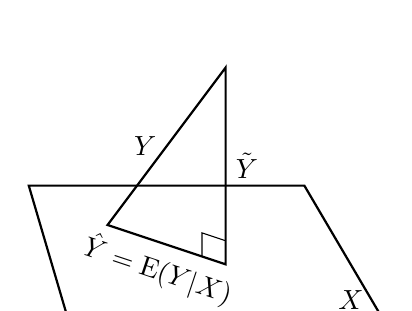
\begin{tikzpicture}
			\draw[thick](0, 0)--(1.5, 2)node[midway, left]{$Y$}--(1.5, -.5)node[midway, right]{$\tilde Y$}--cycle node[midway, sloped, below]{$\hat Y=\E(Y|X)$};
			\draw(1.2, -.4)--(1.2, -.1)--(1.5, -.2);
			\draw[thick](-1, .5)--(2.5, .5)--(3.5, -1.2)node[above left]{$X~$}--(-.5, -1.2)--cycle;
		\end{tikzpicture}
		\tikzchap $Y,\hat Y,\tilde Y$关系示意图
	\end{center}
\end{example}
\begin{definition}{条件方差}{conditional variance}
	定义条件方差
	\begin{align}
		\Var(Y|X):=\E\bigfkh{\bigkh{X-\E(Y|X)}^2|X}
	\end{align}
\end{definition}
自然
\begin{align}
	\Var(Y|X)=\E(Y^2|X)-\E^2(Y|X).
\end{align}
\begin{theorem}{全方差公式}{}
	由例 \ref{exm:error}
	\begin{align}
		\Var(Y)=\E\bigfkh{\Var(Y|X)}+\Var\bigfkh{\E(Y|X)}.
	\end{align}
\end{theorem}
\begin{example}{随机变量个随机变量的和}{}
	随机变量序列$X_1,X_2,\ldots$ iid,$N$是取值为正整数的随机变量,且与$X_i$独立,令$Y=X_1+\cdots+X_N$,则
	\begin{align}
		\E(Y)&=\E\bigfkh{\E(Y|N)}=\E\bigfkh{N\E(X)}=\E(N)\E(X);\\\notag
		\Var(Y)&=\E\bigfkh{\Var(Y|N)}+\Var\bigfkh{\E(Y|N)}\\\notag
		&=\E\bigfkh{N\Var(X)}+\Var\bigfkh{N\E(X)}\\
		&=\Var(X)\E(N)+\E^2(X)\Var(N).
	\end{align}
	特别的,$N\sim\Pois(\lambda)$时,称$Y$为复合Poisson随机变量
	\[
		\Var(Y)=\lambda\bigfkh{\Var(X)+\E^2(X)}=\lambda\E(X^2).
	\]
\end{example}
\clearpage
\section{不等式与极限定理}
\subsection{概率不等式}
\begin{theorem}{Markov不等式}{Markov inequality}
	若随机变量$X>0$,则$\forall\varepsilon>0$,有
	\begin{align}
		\P(X\geqslant\varepsilon)\leqslant\frac{\E(X)}\varepsilon.
	\end{align}
\end{theorem}
\prf 引入示性函数(characteristic function)
\begin{align*}
	I(X\geqslant\varepsilon):=\begin{cases}
		1,&X\geqslant\varepsilon\\
		0,&X<\varepsilon
	\end{cases}
\end{align*}
则$I(X\geqslant\varepsilon)\leqslant X/\varepsilon$,两边取期望,即证。\qed
\begin{theorem}{Chebyshev不等式}{Chebyshev inequality}
	若随机变量$X$方差$\Var(X)$存在,则$\forall\varepsilon>0$
	\begin{align}
		\P(|X-\E(X)|\geqslant\varepsilon)\leqslant\frac{\Var(X)}{\varepsilon^2}.
	\end{align}
\end{theorem}
\prf 由Markov不等式
\begin{align*}
	\P\bigfkh{\bigkh{X-\E(X)}^2\geqslant\varepsilon^2}\leqslant\frac{\E\bigfkh{\bigkh{X-\E(X)}^2}}{\varepsilon^2}\equiv\frac{\Var(X)}{\varepsilon^2}.\rqed
\end{align*}
\begin{theorem}{Chernoff不等式}{Chernoff inequality}
	对随机变量$X$,$\forall\varepsilon>0,\forall t>0$,有
	\begin{align}
		\P(X\geqslant\varepsilon)\leqslant\frac{\E(\e{tX})}{\e{t\varepsilon}}.
	\end{align}
	即使$X$矩母函数不存在,不等式也成立。
\end{theorem}
\prf 由Markov不等式,
\begin{align*}
	\P(X\geqslant\varepsilon)=\P(\e{tX}\geqslant\e{t\varepsilon})\leqslant\frac{\E(\e{tX})}{\e{t\varepsilon}}.\rqed
\end{align*}
\begin{example}{正态分布的尾概率估计}{}
	$X\sim\Norm(0,1)$,则三个不等式给出
	\begin{align*}
		\P(|X|\geqslant 3)\leqslant\begin{cases}
			\frac13\E(X)=\frac13\sqrt{\frac2\pi}\doteq 0.27,&\text{(Markov)}\\[2ex]
			\frac19\Var(X)=\frac19\doteq 0.11,&\text{(Chebyshev)}\\[2ex]
			\frac{2}{\e{3t}}\e{t^2/2}\leqslant 2\e{-9/2}\doteq 0.022.&\text{(Chernoff)}
		\end{cases}
	\end{align*}
	比较而言,Markov仅用到了均值的信息,Chebyshev用到了方差的信息,Chernoff用到了各阶矩的信息。而结果也是越来越好的。
\end{example}
\subsection{大数定律}
为何能以某事件发生的频率作为该事件的概率的估计?
\begin{definition}{依概率收敛}{converge in probability}
	$X_1,X_2,\ldots$为随机变量序列,$X$为随机变量,若$\forall\varepsilon>0$,均有
	\[
		\lim_{n\to\infty}\P(|X_n-X|\geqslant\varepsilon)=0,
	\]
	则称序列$X_n$依概率收敛(converge in probability)于$X$,记作
	\begin{align}
		X_n\pto X.
	\end{align}
\end{definition}
\begin{theorem}{Khinchin弱大数定律}{Khinchin weak law of large numbers}
	随机变量序列$X_1,X_2,\ldots$ iid,且$\E(X_i)=\mu$,则
	\begin{align}
		\avg X_n:=\frac1n\sum_{i=1}^nX_i\pto\mu
	\end{align}
	这就是Khinchin弱大数定律(weak law of large numbers, WLLN).\index{LLN, 大数定律}
\end{theorem}
Khinchin LLN指出:数学期望可以由$n$个iid的随机变量的算术平均值近似。最初的大数定律应用于$X_i\sim\Bern(p)$中用频率$\avg X$估计$p$,这称为Bernoulli LLN。

\begin{example}{用Chebyshev不等式证明Khinchin大数定律}{}
	若方差$\Var(X_i)=\sigma^2$存在\footnote{事实上Khinchin LLN并没有要求$\Var(X_i)$存在。},则
	\begin{align}
		\E(\avg X_n)&=\frac1n\sum_{i=1}^n\E(X_i)=\mu,\\
		\Var(\avg X_n)&=\frac1{n^2}\sum_{i=1}^n\Var(X_i)=\frac{\sigma^2}n.
	\end{align}
	由Chebyshev不等式
	\[
		\P(|\avg X_n-\mu|\geqslant\varepsilon)\leqslant\frac{\sigma^2}{n\varepsilon^2}\to 0.\rqed
	\]
\end{example}

可对Kinchin LLN进行推广:当条件为$X_i$两两不相关,$\Var(X_i)$一致有界时,是Chebyshev LLN;还有Markov LLN。
\begin{definition}{以概率1收敛}{converge almost surely}
	若随机变量序列$X_1,X_2,\ldots$极限存在,且
	\begin{align}
		\P\kh{\lim_{n\to\infty}X_n=X}=1,
	\end{align}
	则称序列$X_n$以概率1收敛(converge almost surely)于$X$,记作
	\begin{align}
		X_n\asto X.
	\end{align}
\end{definition}
可以证明,以概率1收敛是比依概率收敛更强的结论。
\begin{theorem}{Kolmogorov强大数定律}{}
	若$X_1,X_2,\ldots$ iid,$\E(X_i)=\mu$,则 
	\begin{align}
		\avg X_n\asto\mu.
	\end{align}
	芝士Kolmogorov强大数定律(\sout{powerful law of number}, strong law of large numbers, SLLN).
\end{theorem}
SLLN是包含Khinchin WLLN的,但是除了Khinchin,还有其他形式的WLLN。

SLLN说明:概率的频率解释是合理的。也是Monte Carlo积分的原理。

\begin{example}{以概率1收敛强于依概率收敛}{}
	$\Omega=[0,1]$上的均匀分布,从而有$(\Omega,\cF,\P)$,定义
	\begin{align*}
		&Y_1(\omega)=I_{[0,1]}(\omega),\quad\omega\in[0,1]\\
		&Y_2(\omega)=I_{[0,1/2]}(\omega),\enspace Y_3(\omega)=I_{[1/2,1]}(\omega),\\
		&Y_4(\omega)=I_{[0,1/3]}(\omega),\enspace Y_5(\omega)=I_{[1/3,2/3]}(\omega),\enspace Y_6(\omega)=I_{[2/3,1]}(\omega),\\
		&\cdots
	\end{align*}
	显然,$Y_n$依概率收敛到0:
	\[
		\lim_{n\to\infty}\P(|Y_n|\geqslant\varepsilon)=0.
	\]
	但$\lim_{n\to\infty}Y_n$不存在(总有破坏的区间),也就不存在以概率1收敛。
\end{example}
事实上以概率1收敛可以推出依概率收敛,但我就不证了。
\subsection{中心极限定理}
\begin{theorem}{Lindberg-Levi中心极限定理}{Lindberg-Levi central limit theorem}
	随机变量序列$X_1, X_2,\ldots$ iid,且期望$\mu$和方差$\sigma^2$存在。$\avg X$的标准化变量为
	\begin{align}
		Z_n:=\frac{\avg X-\mu}{\sigma/\!\sqrt n}\equiv\sum_{i=1}^n\frac{X_i-\mu}{\sqrt n\sigma}.
	\end{align}
	则$Z_n$的CDF $\CDF_n(z)$极限存在,且
	\begin{align}
		\lim_{n\to\infty}\CDF_n(z)=\Phi(z).\quad\forall z\in\RR
	\end{align}
	其中$\Phi(z)$是$\Norm(0,1)$的CDF,这就是Lindberg-Levi中心极限定理(central limit theorem, CLT)。\index{CLT, 中心极限定理}
\end{theorem}
\prf 标准正态分布的CF $\psi(t)=\e{-t^2/2}$,%不失一般性(without loss of generality, WLOG),
\begin{align*}
	\psi_{Z_n}(t)&=\fkh{\psi_{X_i-\mu}\biggkh{\frac{t}{\sqrt n\sigma}}}^n\\
	&=\fkh{1+0+\frac12\psi''_{X_i-\mu}(0)\cdot\biggkh{\frac{t}{\sqrt n\sigma}}^2+o\biggkh{\frac{t^2}n}}^n\\
	&=\fkh{1-\frac{t^2}{2n}+o\biggkh{\frac{t^2}n}}^n\to\e{-t^2/2}.\rqed
\end{align*}

由CLT,我们可以近似的认为$\avg X\dotsim\Norm(\mu,\sigma^2/n)$。

\begin{example}{DeMoivre-Laplace中心极限定理}{DeMoivre-Laplace central limit theorem}
	特别的,当$X_i\sim\Bern(p)$时,$Y:=X_1+\cdots+X_n\sim\Bern(n,p)$二项分布近似于正态分布$\Norm\bigkh{np,np(1-p)}$
	\[
		\P\kh{Y\leqslant t}\doteq\Phi\kh{\frac{t-np}{\sqrt{np(1-p)}}}.
	\]
	因为正态分布是连续的,对上式进行连续型修正
	\[
		\P(t_1\leqslant Y\leqslant t_2)\doteq\Phi\kh{\frac{t_2-np+1/2}{\sqrt{np(1-p)}}}-\Phi\kh{\frac{t_1-np-1/2}{\sqrt{np(1-p)}}}.
	\]
	这称为DeMoivre-Laplace CLT。
\end{example}
\begin{example}{选举问题}{}
	为统计选民支持度$p$ (未知),随机调查$n$个人,支持比例$P_n=\avg X$,$N\gg n$近似的,可视为有放回$X_i\sim\Bern(p)$,且
	\[
		\frac{P_n-p}{\sqrt{p(1-p)/n}}\sim\Norm(0,1)
	\]
	要求精度$\varepsilon=0.03$,置信度为95\% ($\alpha=0.05$),CLT给出
	\[
		\P(|P_n-p|\geqslant\varepsilon)\doteq 2\fkh{1-\Phi\kh{\frac\varepsilon{\sqrt{p(1-p)/n}}}}\leqslant\alpha
	\]
	当$p=1/2$时$n_{\mathrm{min}}$最大:
	\[
		n_{\mathrm{min}}=\biggkh{\frac{z_{1-\alpha/2}}{2\varepsilon}}^2\doteq 1067.11.
	\]%1.96
	与$N$无关。
\end{example}
\begin{theorem}{Lyapunov中心极限定理}{Lyapunov central limit theorem}
	随机变量序列$X_1,X_2,\ldots$是独立的随机变量序列,且具有期望和方差
	\[
		\E(X_k)=\mu_k,\quad\Var(X_k)=\sigma_k^2;\quad B_n^2:=\sum_{k=1}^n\sigma_k^2.
	\]
	若存在$\delta>0$满足Lyapunov条件:
	\[
		\lim_{n\to\infty}\frac1{B_n^{2+\delta}}\sum_{k=1}^n\E\bigkh{|X_k-\mu_k|}=0.
	\]
	则随机变量之和的标准化变量
	\[
		\hat X_n:=\frac1{B_n}\sum_{k=1}^n(X_k-\mu_k)
	\]
	的CDF
	\[
		\lim_{n\to\infty}\CDF_n(x)=\Phi(x),\quad\forall x\in\RR.
	\]
\end{theorem}
这说明,当$N$很大时,
\begin{align}
	\sum_{i=1}^nX_i\dotsim\Norm\kh{\sum_{i=1}^n\mu_i,\sum_{i=1}^n\sigma^2_i}.
\end{align}

\begin{theorem}{Markov中心极限定理}{}
	随机变量序列$X_1,X_2,\ldots$不独立,但具有Markov性:
	\[
		\P(X_i|X_{i-1}X_{i-2}\cdots)=\P(X_i|X_{i-1}).
	\]
	加上可逆性和可达性的条件,则序列构成一个Markov链,则
	\begin{align}
		\avg X_n\pto Z\dotsim\Norm(\mu,\sigma^2/n)
	\end{align}
\end{theorem}
\paragraph{Review \& Remarks}
\begin{compactenum}
	\item 尾部概率控制;
	\item LLN, CLT;
	\item CLT的应用:$\avg X\dotsim\Norm(\mu,\sigma^2/n),\enspace\sum X_i\dotsim\Norm(n\mu,n\sigma^2)$;
	\item 三种收敛:$\asto,\pto,\dto$\,(依分布收敛)。
\end{compactenum}
\clearpage
\part{统计推断}
\begin{quote}
	\textit{It is better to have an approximate answer to the right question than an exact answer to the wrong one.}

	\rightline{-John Tukey}
\end{quote}
数理统计是从数据到信息的学科
\begin{align*}
	\text{数理统计}\begin{cases}
		\text{数据收集}\\
		\text{数据分析}\begin{cases}
			\text{描述}\\
			\text{推断:样本 }\to\text{ 总体}
		\end{cases}
	\end{cases}
\end{align*}
\section{参数估计}
\begin{definition}{总体}{population}
	总体(population)是指与所研究的问题有关的对象(个体)的全体的某个数值特征$X$的概率分布。
\end{definition}
总体分为有限总体和无限总体。
\begin{definition}{统计模型}{model}
	统计模型(model)是一族概率分布。
\end{definition}
可以通过若干个参数表达出来的模型是参数模型,否则是非参数模型。
\begin{definition}{样本}{sample}
	样本(sample)是随机变量序列$X_1,X_2,\ldots,X_n$,$X_i$取自总体,$n$称为样本容量。
\end{definition}
样本的获取方式:试验、观测。
\begin{definition}{简单随机抽样}{simple random sampling}
	简单随机抽样(simple random sampling)总体个数$N$有限,无放回,任意容量相同的样本都有相同的发生概率。
	\[
		p=\dvd{1}{{N\choose n}}.
	\]
\end{definition}
\begin{definition}{随机样本}{random sample}
	$X_1,\ldots,X_n$ iid,比如有放回抽样
\end{definition}
不当抽样。
\begin{definition}{统计量}{statistic}
	统计量(statistic)是完全由样本决定的量,比如样本期望$\avg X$和样本方差$S^2$
	\[
		\avg X:=\frac1n\sum_{i=1}^nX_i,\quad S^2:=\frac1{n-1}\sum_{i=1}^n(X_i-\avg X)^2.
	\]
\end{definition}
总体决定样本,用样本来推断总体,这就是统计推断。
\subsection{矩估计}
随机样本$X_1,X_2,\ldots$ iid
\begin{definition}{样本矩}{}
	样本$k$阶原点矩
	\[
		a_k:=\frac1n\sum_{i=1}^nX_i^k\pto\E(X^k),
	\]
	$k$阶中心矩
	\[
		m_k:=\frac1n\sum_{i=1}^n(X_i-\avg X)^k\pto\E\bigfkh{(X-\mu)^k},
	\]
\end{definition}
矩估计就是认为总体矩$\doteq$样本矩,从而得到参数的估计。
\begin{example}{正态分布和Poisson分布的矩估计}{}
	iid $X_i\sim\Norm(\mu,\sigma^2)$用样本均值$\avg X$和样本2阶中心矩$m_2$估计
	\begin{align*}
		\begin{cases}
			\mu=\avg X,\\
			\sigma^2=m_2
		\end{cases}
	\end{align*}
	\tcblower
	iid $X_i\sim\Expo(\lambda)$的参数$\lambda$有不止一种估计方法
	\begin{align*}
		\lambda=\frac1{\avg X}\enspace\text{or}\enspace\lambda=\frac1{\sqrt{m_2}}.
	\end{align*}
	但是我们采用低阶矩$\avg X$,因为其受噪声的影响更小。
\end{example}
\subsection{极大似然估计}
假设$X_1,\ldots,X_n$的联合分布为 
\[
	f(x_1,\ldots,x_n;\theta),
\]
其中$\theta$可为标量,也可为向量。
\begin{definition}{似然函数}{likelihood function}
	对于观测$(X_1,\ldots,X_n)$的似然函数(likelihood function)
	\begin{align}
		L(\theta):=f(X_1,\ldots,X_n;\theta).
	\end{align}
\end{definition}
观测数据通常记为$x_1,\ldots,x_n$,称为随机变量$X_1,\ldots,X_n$的一个实现。离散情形,$L(\theta)$即为实现$X_1,\ldots,X_n$的概率。

若$X_1,\ldots,X_n$ iid,总体分布为$g(x;\theta)$,则
\[
	L(\theta)=g(X_1;\theta)\cdots g(X_n;\theta).
\]
\begin{definition}{极大似然估计}{maximum likelihood estimation}
	$\theta$的极大似然估计(maximum likelihood estimation, MLE)为\index{MLE, 极大似然估计}
	\begin{align}
		\theta^\ast:=\mathop{\arg\max}_\theta L(\theta).
	\end{align}
\end{definition}
\begin{example}{正态分布的MLE}{MLE of Normal distribution}
	iid $X_i\sim\Norm(\mu,\sigma^2)$,$\mu,\sigma^2$未知,则其似然函数为
	\[
		L(\mu,\sigma^2)=\prod_{i=1}^n\fkh{\frac1{\sqrt{2\pi}\sigma}\exp\kh{-\frac{(X_i-\mu)^2}{2\sigma^2}}}
	\]
	要求$L$的最大值点,可对$L$求导,然而更方便的做法是求对数似然:
	\[
		\ln L(\mu,\sigma^2)=-\frac n2\ln2\pi-n\ln\sigma-\frac1{2\sigma^2}\sum_{i=1}^n(X_i-\mu)^2.
	\]
	最大值点处满足
	\[
		\begin{cases}
			\pv{\ln L}\mu=0\\[1ex]
			\pv{\ln L}{(\sigma^2)}=0
		\end{cases}\thus
		\begin{cases}
			\mu^\ast=\avg X\\
			(\sigma^2)^\ast=\frac1n\sum(X_i-\avg X)^2.
		\end{cases}
	\]
	经验证,$\mu^\ast,(\sigma^2)^\ast$为所求MLE。
\end{example}
注:MLE具有不变性:
\begin{align}
	\bigkh{g(\theta)}^\ast=g(\theta^\ast).
\end{align}
\begin{example}{均匀分布的MLE}{MLE of Uniform distribution}
	iid $X_i\sim\Unif(0,\theta)$,$\theta$未知
	\[
		L(\theta)=\begin{cases}
			\frac1{\theta^n},&\theta\geqslant X_i>0\\
			0,&\text{elsewhere}
		\end{cases}
	\]
	$\theta^\ast=\max(X_1,\ldots,X_n)$
\end{example}
\begin{example}{Cauchy分布的估计}{estimation of Cauchy distribution}
	估计Cauchy分布的参数$\theta$
	\[
		f(x;\theta)=\frac1\pi\frac1{1+(x-\theta)^2},\quad x\in\RR
	\]
	期望不存在,无矩。
	
	似然方程
	\[
		\dv{\ln L}\theta=0,\thus\sum_{i=1}^n\frac{X_i-\theta}{1+(X_i-\theta)^2}=0.
	\]
	当$n>2$时很难解。回到参数的意义,$\theta$可用样本中位数估计。
\end{example}
估计方法不唯一,即使MLE也不一定唯一,MLE需要$f$ (分布的参数形式),算法。

\subsection{Bayes估计}
矩估计和MLE都是点估计,将参数$\theta$被视为未知的数(组)。
若对参数$\theta$有先验知识,可用随机变量$\varTheta$的概率分布来刻画,称之为先验分布(priori distribution)
\[
	f_\varTheta(\theta)
\]
$\theta$是$\varTheta$的实现值;$X$是实验(观测)结果,样本分布为
\[
	f_{X|\varTheta}(x|\theta)
\]
由Bayes公式,后验分布(posterior distribution)为
\begin{align}
	f_{\varTheta|X}(\theta|X)=\frac{f_\varTheta(\theta)f_{X|\varTheta}(x|\theta)}{f_X(x)}=\frac{f_\varTheta(\theta)f_{X|\varTheta}(x|\theta)}{\textstyle\int_\theta f_\varTheta(\theta)f_{X|\varTheta}(x|\theta)\d\theta}.
\end{align}
若$\varTheta\sim\Unif,f_\varTheta(\theta)\propto 1$,称为Bayes法则,也叫同等无知原则。
\begin{example}{二项分布的Bayes估计}{}
	$X=n$次掷币正面向上次数,当$\varTheta=\theta$时,$X\sim\Bern(n,\theta)$
	\[
		f_{X|\varTheta}(x|\theta)={n\choose x}\theta^x(1-\theta)^{n-x},\quad x=0,1,\ldots,n.
	\]
	采用Bayes法则,$(X,\varTheta)$的联合分布PDF为
	\[
		f_{X,\varTheta}(x,\theta)=f_{\varTheta}(\theta)f_{X|\varTheta}(x|\theta)={n\choose x}\theta^x(1-\theta)^{n-x},\quad\theta\in(0,1).
	\]
	所以
	\begin{align*}
		f_X(x)&={n\choose x}\int_0^1\theta^x(1-\theta)^{n-x}\d\theta\\
		&={n\choose x}\mathrm B(x+1,n-x+1)=\frac1{n+1}.
	\end{align*}
	故后验概率
	\[
		f_{\varTheta|X}(\theta|x)=\frac{(n+1)!}{x!(n-x)!}\theta^x(1-\theta)^{n-x}.
	\]
	故$\theta\sim\mathrm{Be}(x+1,n-x+1)$,
	
	\[
		\hat\theta=\E(\varTheta|x)=\frac{x+1}{n+2}.
	\]
	或
	\[
		\theta^\ast=\arg\max f_{\varTheta|X}(\theta|x)=\frac xn.
	\]
	\tcblower
	上面取得先验分布为$\Unif(0,1)=\mathrm{Be}(1,1)$,若先验分布取为$\mathrm{Be}(a,b)$,则后验分布为$\mathrm{Be}(a+x,b+n-x)$
\end{example}
需要注意,这里的先验分布并不是唯一指定的。
\subsection{无偏性}
\begin{definition}{偏差}{bias}
	统计量
	\[
		\hat\theta=\hat\theta(X_1,\ldots,X_n).
	\]
	是对$\theta$的一个估计,定义偏差(bias)%\index{bias, 偏差}
	\begin{align}
		\E(\hat\theta-\theta)=\E(\hat\theta)-\theta.
	\end{align}
	若$\forall\theta,\enspace\E(\hat\theta)=\theta$,则$\hat\theta$是$\theta$的一个无偏估计(unbiased estimation)。
\end{definition}
$\hat g(X_1,\ldots,X_n)$是$g(\theta)$的无偏估计当
\[
	\E(\hat g)=g(\theta),\quad\forall\theta.
\]
若无偏,由LLN
\[
	\frac1{N}\sum_{n=1}^N\hat g(X_1^{(n)},\ldots,X_n^{(n)})\asto\E(\hat g)=g(\theta).
\]
\begin{example}{样本期望、方差的无偏性}{unbiasedness sample expectation and variance}
	样本均值的期望和方差
	\begin{align}
		\E(\avg X)&=\frac1n\sum_{i=1}^n\E(X_i)=\mu,\\
		\Var(\avg X)&=\frac1{n^2}\sum_{i=1}^n\Var(X_i)=\frac{\sigma^2}n.
	\end{align}
	样本方差,由定义
	\[
		S^2=\frac1{n-1}\sum_{i=1}^n(X_i-\avg X)^2=\frac1{n-1}\kh{\sum_{i=1}^nX_i^2-n\avg X^2}
	\]
	的均值
	\begin{align}\notag
		\E(S^2)&=\frac n{n-1}\fkh{\frac1n\sum_{i=1}^n\E(X_i^2)-\E(\avg X^2)}\\
		&=\frac n{n-1}\fkh{\sigma^2+\mu^2-\kh{\frac{\sigma^2}n+\mu^2}}=\sigma^2.
	\end{align}
\end{example}
\begin{example}{均匀分布的无偏估计}{unbiased estimation of Uniform distribution}
	在例 \ref{exm:MLE of Uniform distribution} 中给出了均匀分布$\Unif(0,
	\theta)$的MLE 
	\[
		\theta^\ast=\max(X_1,\ldots,X_n).
	\] 
	这种估计是有偏的,可以证明
	\[
		\E(\theta^\ast)=\frac n{n+1}\theta.
	\]
	以下四种估计都是无偏的:
	\begin{align*}
		\hat\theta_1&:=\frac{n+1}n\max(X_1,\ldots,X_n).\\
		\hat\theta_2&:=\max(X_1,\ldots,X_n)+\min(X_1,\ldots,X_n),\\
		\hat\theta_3&:=2\avg X,\enspace\text{(矩估计)}\\
		\hat\theta_4&:=(n+1)\min(X_1,\ldots,X_n).
	\end{align*}
	但其精确度越来越差。
\end{example}
\subsection{均方误差准则}
\begin{definition}{均方误差}{mean square error}
	定义均方误差(mean square error, MSE)\index{MES, 均方误差}
	\begin{align}
		\E\bigfkh{(\hat\theta-\theta)^2}=\Var(\hat\theta)+\E^2(\hat\theta-\theta).
	\end{align}
\end{definition}
%由定义可以看出,
MSE由两部分构成,$\Var(\hat\theta)$表示$\hat\theta$的精确度(precision),$\E^2(\hat\theta-\theta)$代表准确度(accuracy)。无偏估计后者为0。
\begin{definition}{有效性}{}
	假定$\hat\theta_1,\hat\theta_2$是$\theta$的无偏估计,若
	\[
		\Var(\hat\theta_1)\leqslant\Var(\hat\theta_2),\quad\forall\theta
	\]
	且存在一个分布(i.e.一个$\theta$值)使得$<$成立,则称在MSE意义下,$\hat\theta_1$比$\hat\theta_2$更有效。
\end{definition}
如果所有无偏估计中存在最小的方差,则称为一致最小方差无偏估计(uniformly minimum variance unbiased estimator, UMVUE)。
\begin{theorem}{Cramer-Rao下限}{}
	任何$\theta$的无偏估计量满足
	\begin{align}
		\Var(\hat\theta)\geqslant\frac1{I_n(\theta)}.
	\end{align}
	其中$I_n(\theta)$是Fisher信息量,见定义 \ref{dfn:Fisher information}
\end{theorem}
\begin{example}{低偏倚换方差}{}
	总体$X\sim\Norm(\mu,\sigma^2)$,样本方差$S^2$是无偏的,而样本二阶矩$m_2$是有偏的,
	但MSE
	\[
		\E\bigfkh{(m_2-\sigma^2)^2}<\E\bigfkh{(S^2-\sigma^2)^2}.
	\]
\end{example}
\subsection{大样本性质}
$\hat\theta=\hat\theta(X_1,\ldots,X_n)$当样本容量$n\to\infty$时的性质,

\begin{definition}{渐进无偏性}{}
	$n\to\infty$时,
	\begin{align}
		\E(\hat\theta)\to\theta.
	\end{align}
\end{definition}
\begin{definition}{相合性}{consistent}
	称$\hat\theta$为$\theta$的(弱)相合估计(consistent estimate)当
	\begin{align}
		\hat\theta\pto\theta.
	\end{align}
\end{definition}
WLLN指出,$\avg X$为$\mu$的一个相合估计。相合性为良好点估计的自然要求。
\begin{example}{二阶中心矩}{}
	二阶中心矩$m_2$是总体方差$\sigma^2$的相合估计。
	\begin{align*}
		m_2&=\frac1n\sum_{i=1}^n(X_i-\avg X)^2\\
		&=\frac1n\sum_{i=1}^n(X_i-\mu)^2-(\avg X-\mu)^2\pto\sigma^2+0.
	\end{align*}
\end{example}
\begin{definition}{渐进正态性}{}
	若$\exists\sigma_n>0$使得
	\begin{compactenum}
		\item $\lim_{n\to\infty}\sigma_n=0;$
		\item $\lim_{n\to\infty}\P\biggl(\frac{\hat\theta-\theta}{\sigma_n}\leqslant x\biggr)=\Phi(x).$
	\end{compactenum}
	则称$\hat\theta$为$\theta$的相合近似正态估计。
\end{definition}
\begin{compactenum}
	\item 有时,取$\sigma_n^2=\Var(\hat\theta)$,比如用$\avg X$估计$\mu$;
	\item $n\gg 1$时,$\hat\theta\dotsim\Norm(\theta,\sigma_n^2).$;
	\item 原式分布(即$X_i$的分布) $f$满足光滑性条件,则$\exists\sigma_n>0$使得
	\begin{align}\label{MLE-dto-N01}
		\frac{\theta^\ast-\theta}{\sigma_n}\dto\Norm(0,1).
	\end{align}
\end{compactenum}
\begin{definition}{Fisher信息量}{Fisher information}
	$X_1,\ldots,X_n$ iid,对数似然函数
	\[
		\ell(\theta):=\ln f(X;\theta)=\sum_{i=1}^n\ln f(X_i;\theta).
	\]
	定义Fisher信息量
	\begin{align}
		I_n(\theta)&:=\E(\ell'^2).
	\end{align}
\end{definition}
Fisher信息量是衡量观测所得的随机变量$X$携带的关于未知参数$\theta$的信息量,其中$X$的概率分布依赖于参数$\theta$。

$\ell(\theta)$导数的期望
\[
	\E(\ell')=\int\frac1f\pv f\theta\cdot f\d x=\pp\theta\int f\d x\equiv 0.
\]
二阶导期望
\[
	\E(\ell'')=\E\biggl[\frac1f\pv[2]f\theta-\biggl(\frac1f\pv f\theta\biggr)^2\biggr]=0-\E(\ell'^2)=-\Var(\ell').
\]
Fisher信息量与样本容量有关:
\[
	I_n(\theta)=\sum_{i=1}^n\E\biggl[\biggl(\pp\theta\ln f(X_i;\theta)\biggr)^2\biggr]=nI_1(\theta)=:nI(\theta).
\]
\begin{example}{Fisher信息量证明式(\ref{MLE-dto-N01})}{}
	由MLE的性质,$\ell'(\theta^\ast)=0$,做Talyor展开,
	\[
		0=\ell'(\theta^\ast)=\ell'(\theta)+(\theta^\ast-\theta)\ell''(\theta)+\cdots
	\]
	故
	\[
		\theta^\ast-\theta\doteq-\frac{\ell'(\theta)}{\ell''(\theta)}.
	\]
	设$\ell'(\theta)=n\avg Y$,
	\[
		Y_i:=\pp\theta\ln f(X_i;\theta),\quad\E(Y_i)=0,\enspace\Var(Y_i)=I(\theta).
	\]
	CLT说明,$\avg Y$是渐进正态的,故分子
	\[
		\frac1{\sqrt n}\ell'(\theta)=\sqrt n\,\avg Y\dto\Norm\bigkh{0,I(\theta)}.
	\]
	分母
	\[
		\frac1n\ell''(\theta)\pto I(\theta).
	\]

	故$\theta^\ast-\theta$是渐进正态的:
	\[
		\sqrt n(\theta^\ast-\theta)\dto\Norm\kh{0,\frac1{I(\theta)}}.
	\]
	式(\ref{MLE-dto-N01})中的 
	\[
		\sigma_n=\frac1{\sqrt{nI(\theta)}}~\text{或}~\frac1{\sqrt{nI(\theta^\ast)}}
	\]
\end{example}
\paragraph{Review}
\begin{compactenum}
	\item 参数估计:样本$X_1,\ldots,X_n$,通常假设iid
	
	样本分布$f(x_1,\ldots,x_n;\theta)$即$X_1,\ldots,X_n$的联合分布

	估计$\hat\theta=\hat\theta(X_1,\ldots,X_n)$是统计量,样本的函数

	标准误差:$\hat\theta$的标准差
	\begin{align}
		se(\hat\theta):=\sqrt{\Var(\hat\theta)}.
	\end{align}
	标准误差的估计$\hat{se}=\hat{se}(\hat\theta)$
	\item 经典估计的优良性:
	
	$n$固定:无偏性、有效性;

	$n\to\infty$:渐进无偏性、相合性、渐进正态性。

	\item Bayes估计:将$\theta$理解成一个随机变量$\varTheta$的实现值。$\varTheta$刻画了对$\theta$的认知
	\[
		f_\varTheta(\theta)\turnto f_{\varTheta|X}(\theta|x),
	\]
	后验众数v.s. MLE。Bayes假设二者相等。
\end{compactenum}
\subsection{区间估计}
\begin{definition}{置信区间}{}
	给定$\alpha\in(0,1)$,$\forall\theta$可能值,有$\hat\theta_1,\hat\theta_2$使得
	\begin{align}
		\P(\hat\theta_1<\theta<\hat\theta_2)\geqslant1-\alpha.
	\end{align}
	这里$\hat\theta_i=\hat\theta_i(X_1,\ldots,X_n)$,则称$(\hat\theta_1,\hat\theta_2)$为$\theta$的$(1-\alpha)$置信的区间估计。
\end{definition}
$\alpha$通常取0.05, 0.01, 0.1,可靠性优先。
\begin{definition}{枢轴变量}{}
	仅含一个待估参数的样本的连续函数,且分布不依赖于未知参数。
\end{definition}
\begin{method}{枢轴变量法}{}
	\begin{compactenum}
		\item 确定$\hat\theta$;
		\item 找到枢轴变量$H(\hat\theta,\theta)$的分布可用;
		\item 确定$(\hat\theta_1,\hat\theta_2)$
	\end{compactenum}
\end{method}
\begin{example}{正态分布的区间估计}{}
	$X\sim\Norm(\mu,\sigma^2)$的$\sigma^2$已知,$\mu$未知,由$\avg X\sim\Norm(\mu,\sigma^2/n)$,
	取枢轴变量
	\[
		Z:=\frac{\avg X-\mu}{\sigma/\sqrt n}\sim\Norm(0,1)
	\]
	取对称的上下限
	\[
		\P\kh{\abs Z\geqslant z_{\alpha/2}}=\alpha,\thus\Phi(z_{\alpha/2})=1-\alpha/2
	\]
	其中$z_{\alpha/2}$是$\Norm(0,1)$的上$\alpha/2$分位数。
	故$\mu$的$(1-\alpha)$置信区间为
	\begin{align}
		\kh{\avg X\pm z_{\alpha/2}\frac\sigma{\sqrt n}}.
	\end{align}
	%若$\alpha=0.05$,则$z_{0.025}=1.96$
	%若要求误差不超过$\varepsilon$,则
	%n=\frac{z_{\alpha/2}^2\sigma^2}{\varepsilon^2}
	\tcblower
	若$\mu,\sigma^2$均未知,需要用$S^2$估计$\sigma^2$,由式(\ref{sample-chi2})
	\[
		\chi^2:=\frac{(n-1)S^2}{\sigma^2}\sim\chi^2(n-1),
	\]
	卡方分布并不对称,我们选择等尾置信区间,即
	\[
		\P\bigkh{\chi^2<\chi_{\alpha/2}^2(n-1)}=\P\bigkh{\chi^2>\chi_{1-\alpha/2}^2(n-1)}=\frac\alpha{2},
	\]
	$\sigma^2$的$(1-\alpha)$置信区间为
	\begin{align}
		\kh{\frac{(n-1)S^2}{\chi_{\alpha/2}^2(n-1)},\frac{(n-1)S^2}{\chi_{1-\alpha/2}^2(n-1)}};
	\end{align}

	对$\mu$的估计,由式(\ref{sample-t})
	\[
		t:=\frac{\avg X-\mu}{S/\sqrt n}\sim\mathrm t(n-1).
	\]
	%\P\bigkh{\abs G\geqslant t_{\alpha/2}(n-1)}=\alpha.
	可得$\mu$的$(1-\alpha)$置信区间为
	\begin{align}
		\kh{\avg X\pm t_{\alpha/2}(n-1)\frac{S}{\sqrt n}}.
	\end{align}
\end{example}
\begin{center}
	\tablechap{区间估计}
	\begin{tabular}{cccc}
		\toprule
		条件&估计&枢轴量&置信区间\\
		\midrule
		$\sigma^2$已知&$\mu$&$\frac{\avg X-\mu}{\sigma/\sqrt n}$&$\kh{\avg X\pm z_{\alpha/2}\frac\sigma{\sqrt n}}$\\[2ex]
		$\sigma^2$未知&$\mu$&$\frac{\avg X-\mu}{S/\sqrt n}$&$\kh{\avg X\pm t_{\alpha/2}(n-1)\frac S{\sqrt n}}$\\[2ex]
		$\mu$未知&$\sigma^2$&$\frac{(n-1)S^2}{\sigma^2}$&$\biggl(\frac{(n-1)S^2}{\chi_{\alpha/2}^2(n-1)},\frac{(n-1)S^2}{\chi_{1-\alpha/2}^2(n-1)}\biggr)$\\
		\bottomrule
	\end{tabular}
\end{center}
同理可求单侧置信限,如$\sigma^2$已知时$\mu$的上、下单侧置信限分别为
\[
	\overline\mu=\avg X+z_\alpha\frac\sigma{\sqrt n},\quad\underline\mu=\avg X-z_\alpha\frac\sigma{\sqrt n}.
\]
\begin{example}{两个正态总体}{}
	$X\sim\Norm(\mu_1,\sigma^2),Y\sim\Norm(\mu_2,\sigma^2)$独立,$\mu_1,\mu_2,\sigma^2$未知,估计$\mu_1-\mu_2$
	\begin{align*}
		\avg X-\mu_1-(\avg Y-\mu_2)&\sim\Norm\Bigkh{0,\frac{\sigma^2}{n_1}+\frac{\sigma^2}{n_2}};\\
		\frac{(n_1-1)S_1^2}{\sigma^2}+\frac{(n_2-1)S_2^2}{\sigma^2}&\sim\chi^2(n_1+n_2-2).
	\end{align*}
	利用t分布的定义,构造枢轴变量:
	\[
		H:=\frac{\avg X-\mu_1-(\avg Y-\mu_2)}{S_w\sqrt{\frac1{n_1}+\frac1{n_2}}}\sim\mathrm t(n_1+n_2-2)
	\]
	其中 
	\[
		S_w:=\sqrt{\frac{(n_1-1)S_1^2+(n_2-1)S_2^2}{n_1+n_2-2}}
	\]
	$\mu_1-\mu_2$的$(1-\alpha)$置信区间为
	\[
		\kh{\avg X-\avg Y\pm t_{\alpha/2}(n_1+n_2-2)S_w\sqrt{\frac1{n_1}+\frac1{n_2}}}
	\]
\end{example}
\paragraph{大样本方法}
渐进置信区间
\begin{example}{选举问题的置信区间估计}{}
	真实支持率$p$未知,$n=1200$,观测比例
	\[
		\frac{684}{1200}\doteq 0.57
	\]
	给出$p$的一个95\% 置信区间。

	近似有放回:$X_i\sim\Bern(p)$ iid,$P_n=\avg X$,故
	\[
		\E(P_n)=p,\quad\Var(P_n)=\frac{p(1-p)}n
	\]
	由CLT,
	\[
		\frac{P_n-p}{\sqrt{p(1-p)/n}}\dotsim\Norm(0,1).
	\]
	由于$p$未知,这个方法不能直接用,需要进行一个好的估计。
	\begin{compactenum}[I]
		\item 用$S^2$估计$\sigma^2=p(1-p)$,则标准误差
			\[
				\hat{se}=\sqrt{\frac{S^2}n}=0.2475.
			\]
			可认为
			\[
				\frac{P_n-p}{\hat{se}}\dotsim\Norm(0,1).
			\]
			$p$的95\%置信区间
			\[
				(P_n\pm z_{\alpha/2}\hat{se})=(0.542,0598)
			\]
		\item 用$m_2$估计$\sigma^2$,
			\begin{align*}
				m_2&=\frac1n\sum_{i=1}^n(X_i-\avg X)^2\\
				&=P_n(1-P_n)^2+(1-P_n)(0-P_n)^2=P_n(1-P_n).
			\end{align*}
			相当于用$P_n$估计$p$,估计结果与I相同。
		\item (Naïve)用$1/4$估计$p(1-p)$,此时$\hat{se}=1/\sqrt{4n}$,估计结果为$(0.542,0.599).$
		\item (不具有推广性)由于 
		\[
			\abs{P_n-p}=z_{\alpha/2}\sqrt{\frac{p(1-p)}n},
		\]
		可以解出$p_\pm$,区间$(p_-,p_+)=(0.542,0598).$
	\end{compactenum}
\end{example}
\begin{example}{相合估计}{}
	上例,极大似然估计$P^\ast=P_n$,由MLE的渐进正态性
	\[
		\frac{P^\ast-P}{\sigma_n^2}\dotsim\Norm(0,1)
	\]
	$f(X_i;p)=p^{X_i}(1-p)^{1-X_i}$,故
	\[
		\pp p\ln f(X_i;p)=\frac{X_i}p-\frac{1-X_i}{1-p}=\frac{X_i-p}{p(1-p)}.
	\]
	Fisher信息量
	\[
		I(p)=\E\biggfkh{\biggkh{\frac{X_i-p}{p(1-p)}}^2}=\frac1{p(1-p)}.
	\]
	则
	\[
		\frac{P^\ast-p}{1/\sqrt{nI(p)}}\dotsim\Norm(0,1).
	\]
	可以用$I(P^\ast)$估计$I(p)$,即
	\[
		\frac{P_n-p}{\sqrt{P_n(1-P_n)/n}}\dotsim\Norm(0,1)
	\]
\end{example}
\begin{example}{两个正态总体的相合估计}{}
	$X\sim\Norm(\mu_1,\sigma_1^2),Y\sim\Norm(\mu_2,\sigma_2^2)$独立,自然
	\[
		\frac{\avg X-\mu_1-(\avg Y-\mu_2)}{\sqrt{\frac{\sigma_1^2}{n_1}+\frac{\sigma_2^2}{n_2}}}\sim\Norm(0,1).
	\]
	可估计
	\[
		\frac{\avg X-\mu_1-(\avg Y-\mu_2)}{\sqrt{\frac{S_1^2}{n_1}+\frac{S_2^2}{n_2}}}\dotsim\Norm(0,1).
	\]
\end{example}
\subsection{Beyas区间估计}
有了$\varTheta$的后验分布$f_{\varTheta|X}(\theta|x)$
\[
	\P(a<\varTheta<b|x)=1-\alpha.
\]

最大后验区间满足
\[
	f_{\varTheta|X}(a|x)=f_{\varTheta|X}(b|x).
\]
等尾可信区间满足
\[
	\P(\varTheta<a|x)=\P(\varTheta>b|x)=\frac\alpha{2}.
\]
\paragraph{Review}
\begin{compactenum}
	\item 不管是连续还是离散分布,它们的参数都是连续的。
	\item 置信区间 v.s. Bayes区间(可信区间)
	\[
		\P(\hat\theta_1<\theta<\hat\theta_2)\geqslant 1-\alpha,\quad\hat\theta_i=\hat\theta_i(X_1,\ldots,X_n)\text{——统计量}
	\]
	$(\hat\theta_1,\hat\theta_2)$——随机区间。当得到样本具体观测值$(x_1,\ldots,x_n)$代入$\hat\theta_1,\hat\theta_2$得到具体区间。
	\[
		\P(a<\varTheta<b|x)=1-\alpha.
	\]
	后验分布
	\item 小样本方法v.s.大样本方法:精确分布v.s.近似分布
\end{compactenum}
\clearpage
\section{假设检验}
\begin{example}{零件检测}{component test}
	一大批电子元件寿命$X$,样本$X_1,\ldots,X_n$
	\begin{compactenum}
		\item 若假设$X\sim\Expo(\lambda)$,那么$\lambda=\,?$

		回答:参数估计
		\item 若合格标准为$\E(X)\geqslant 5000$,那么如何判断这一批是否合格?
		
		尝试回答:建立执行标准,比如样本$\avg X>\ell$,那么$\ell=\,?$

		%样本多大程度上支持假设?
	\end{compactenum}
\end{example}
参数估计是对参数一无所知;假设检验是对参数有所了解,但有怀疑猜测需要证实。
\subsection{基本概念}
\begin{definition}{统计假设}{hypothesis}
	假设(hypothesis)是对一个或多个总体的某种推断或猜测。
	\begin{compactitem}
		\item 原假设(null hypothesis) $H_0$:被检验的假设;
		\item 备择假设(alternative \textasciitilde) $H_1$:拒绝$H_0$后可供选择的假设。
	\end{compactitem}
	简单假设:只对应一个总体;复合假设:对应多个总体
\end{definition}
若假设可表示为参数形式,则
\[
	H_0:\theta\in\varTheta_0,\quad H_1:\theta\in\varTheta_1
\]
其中$\varTheta_0\cap\varTheta_1=\varnothing,\enspace\varTheta_0\cup\varTheta_1=\{\theta\,\text{的所有可能取值(应用角度)\}}$。
\begin{example}{}{}
	接例 \ref{exm:component test},
	\[
		H_0:\mu\geqslant\mu_0,\quad H_1:\mu<\mu_0,
	\]
	$H_0$是复合假设,单侧检验(看$H_1$)。
	\tcblower
	$X\sim\Norm(\mu,\sigma_0^2)$,
	\[
		H_0:\mu=\mu_0,\quad H_1:\mu\neq\mu_0,
	\]
	$H_0$是简单假设($\sigma_0^2$已知的情况下),双侧检验(看$H_1$)。
\end{example}

$H_0$往往是受保护的,无充分证据不能拒绝;$H_1$往往是真正感兴趣的。
\begin{theorem}{小概率原理}{}
	在假设$H_0$为真的情况下,所观测的样本出现的概率如果很小,意味着样本提供的证据拒绝$H_0$。
	%概率很小的事件在一次试验中是不会发生的;在一次试验中小概率事件如果发生了,我们就有理由认为提出的$H_0$是不对的。
\end{theorem}
%小概率由研究者事先确定,一般取1\%, 5\%或10\%。小概率的取值不同,假设检验的结果可能不同。
在统计学中,小概率又叫\textbf{显著性水平},因此,假设检验又称为\textbf{显著性检验}。一般来说,我们都希望拒绝$H_0$得到所谓的显著性差异。
\begin{definition}{假设检验}{hypothesis test}
	检验(准则):做出决策的一个具体法则。

	$R$:临界域(或拒绝域,critical region),形式上可抽象为
	\[
		R=\set{(X_1,\ldots,X_n)}{T(X_1,\ldots,X_n)\geqslant c}.
	\]
	$c$称为临界值。
\end{definition}

\begin{definition}{两类错误}{}
	\begin{compactenum}[I]
		\item 弃真错误:$H_0$为真时拒绝$H_0$,概率 
		\begin{align}
			\alpha(R):=\P_\theta\bigkh{(X_1,\ldots,X_n)\in R},\quad \theta\in\varTheta_0
		\end{align}
		\item 取伪错误:$H_0$为假时接受$H_0$,概率
		\begin{align}
			\beta(R):=\P_\theta\bigkh{(X_1,\ldots,X_n)\notin R},\quad \theta\in\varTheta_1
		\end{align}
	\end{compactenum}
\end{definition}
依据样本决策,错误不可避免。当$n$固定时,$\alpha,\beta$不能同时变小。
\begin{center}
	\begin{tikzpicture}[xscale=1.5, yscale=1.5]
		\node at(-2, .5){$H_0$为真};
		\node at(-2, -1){$H_0$为假};
		\fill[gray](1, 0)--(1, .368)--(2, .02)node[midway, above]{$\alpha$}--(2, 0);
		\fill[white, domain=1:2]plot(\x,{exp(-\x*\x)});
		\fill[gray, shift={(1.75, -1.5)}](-.75, 0)--(-.75, .57)--(-2, .02)node[midway, above]{$\beta$}--(-2, 0);
		\fill[white, domain=-2:-.75, shift={(1.75, -1.5)}]plot(\x,{exp(-\x*\x)});
		\draw[dashed](1, 1)--(1, -1.5);
		\draw[thick, -latex](-1.75, 0)--(3.5, 0)node[right]{$x$};
		\draw(0, .05)--(0, 0)node[below]{$\mu_0$};
		\draw[thick, domain=-1.5:2, samples=100]plot(\x,{exp(-\x*\x)});
		\draw[thick, -latex](-1.75, -1.5)--(3.5, -1.5)node[right]{$x$};
		\draw[thick, domain=-2:1.5, samples=100, shift={(1.75, -1.5)}]plot(\x,{exp(-\x*\x)});
	\end{tikzpicture}
	\tikzchap I类错误和II类错误示意图
\end{center}
\begin{definition}{功效函数}{power function}
	定义功效函数(power function)是样本落在$R$上的概率
	\begin{align}
		\P_\theta\bigkh{(X_1,\ldots,X_n)\in R}=\begin{cases}
			\alpha(R),&\theta\in\varTheta_0\\
			1-\beta(R),&\theta\in\varTheta_1
		\end{cases}
	\end{align}
	功效指在$H_1$成立时拒绝$H_0$的概率,即$1-\beta(R)$,越大越好。
\end{definition}
\begin{theorem}{Neyman-Pearson范式}{Neyman-Pearson normal form}
	($n$固定)预先给定检验水平$\alpha>0$,控制
	\[
		\alpha(R)\leqslant\alpha,\enspace\forall\theta\in\varTheta_0,
	\]
	再在这个限制下使$\beta(R)$尽可能小。
\end{theorem}
$\alpha$固定时,使$\beta(R)$最小的检验称为水平$\alpha$下的\textbf{一致最优检验}(不一定存在,即使存在一般也不易求)


\subsection{临界值检验法}
\begin{method}{临界值检验法}{}
	\begin{compactenum}
		\item 提出假设$H_0,H_1$
		\item 给定$\alpha>0$
		\item 选择检验统计量,确定拒绝域形状(由$H_1$决定)
		\item 构建检验:$\alpha(R)\leqslant\alpha\rightsquigarrow R$
		\item 采样,计算检验统计量的值
		\item 代入检验准则,进行决策
	\end{compactenum}
\end{method}
这个过程缺少对于功效$1-\beta(R)$的讨论。
\begin{example}{$Z$检验法和$t$检验法}{Z test & t test}
	$X\sim\Norm(\mu,\sigma^2)$,$\sigma^2$已知, 
	\[
		H_0:\mu=\mu_0,\quad H_1:\mu\neq\mu_0,
	\]
	当$H_0$为真时,由式(\ref{sample-N}),选择统计量
	\[
		Z:=\frac{\avg X-\mu_0}{\sigma/\sqrt n}\sim\Norm(0,1),
	\]
	显著性水平$\alpha>0$给定,检验的拒绝域为
	\[
		C=\set{Z}{\abs Z\geqslant z_{\alpha/2}}.
	\]
	这被称为$Z$检验法。
	\tcblower
	当$\sigma^2$未知时,就需要选择统计量
	\[
		t:=\frac{\avg X-\mu_0}{S/\sqrt n}\sim\mathrm t(n-1),
	\]
	相应的,检验的拒绝域为
	\[
		C=\set{Z}{\abs t\geqslant t_{\alpha/2}(n-1)}.
	\]
	这被称为$t$检验法。
\end{example}
\begin{center}
	\tablechap{假设检验}
	\begin{tabular}{cccc}
		\toprule
		条件&$H_0$&统计量&拒绝域\\
		\midrule
		$\sigma^2$已知&$\mu=\mu_0$&$Z:=\frac{\avg X-\mu_0}{\sigma/\sqrt n}\sim\Norm(0,1)$&$\abs Z\geqslant z_{\alpha/2}$\\[2ex]
		$\sigma^2$未知&$\mu=\mu_0$&$t:=\frac{\avg X-\mu_0}{S/\sqrt n}\sim\mathrm t(n-1)$&$\abs t\geqslant t_{\alpha/2}(n-1)$\\[2ex]
		\multirow{2}*{$\mu$未知}&\multirow{2}*{$\sigma^2=\sigma_0^2$}&\multirow{2}*{$\chi^2:=\frac{(n-1)S^2}{\sigma_0^2}\sim\chi^2(n-1)$}&$\chi^2\geqslant\chi^2_{\alpha/2}(n-1)$或\\
		&&&$\chi^2\leqslant\chi^2_{1-\alpha/2}(n-1)$\\
		\bottomrule
	\end{tabular}
\end{center}
当$H_0$形如$\mu\geqslant\mu_0$时,进行单侧检验。
\paragraph{Review}
\begin{compactenum}
	\item $H_0$ v.s. $H_1$,二者天然不对等
	
	若认可某一组样本,则用它来证实或证伪某理论(推测);
	\item 决策:拒绝$H_0$或不拒绝$H_0$
	
	检验(准则) =决策准则,拒绝域$R$的划分
	\item 统计学中没有绝对的证实或证伪,
	
	$\alpha,\beta$属于检验程序的属性,而非样本的属性。
	
	$\alpha(R)\leqslant\alpha,\beta(R)\leqslant\beta$预先指定的可接受的长期错误率。
	\item 功效函数v.s.功效,
	
	不拒绝v.s.接受:$\beta(R)$小(功效大),当样本支持$H_0$,才能接受$H_0$;通常人们忽略了对II类错误的系统控制,将导致对结果意义以及下一步工作方向的误判。
	\item 临界值检验法。缺少对功效的讨论
\end{compactenum}
\subsection{临界值检验与置信区间的对偶关系}
\begin{example}{正态分布的临界值检验与置信区间}{}
	$X\sim\Norm(\mu,\sigma^2)$,$\sigma^2$已知,$\alpha\in(0,1)$给定,$X_1,\ldots,X_n$ iid 

	(双侧)置信区间
	\[
		\mu\in\kh{\avg X\pm z_{\alpha/2}\frac\sigma{\sqrt n}}.
	\]
	假设检验:考虑
	\[
		H_0:\mu=\mu_0,\quad H_1:\mu\neq\mu_0.
	\]
	%由
	%\P_{\mu=\mu_0}\Bigkh{\abs{\avg X-\mu_0}\geqslant c}\leqslant\alpha
	检验:%当$\abs{\avg X-\mu_0}\geqslant z_{\alpha/2}\sigma/\sqrt n$时拒绝$H_0$,
	接受域
	\[
		R\c=\set{(X_1,\ldots,X_n)}{\abs{\avg X-\mu_0}<z_{\alpha/2}\frac\sigma{\sqrt n}}.
	\]
\end{example}
\begin{theorem}{临界值检验与置信区间的对偶关系}{}
	\begin{center}
		置信区间包含$\mu_0$\\
		$\Updownarrow$\\
		用$\avg X$做检验统计量,建设检验$H_0:\mu=\mu_0\enspace H_1:\mu\neq\mu_0$不拒绝$H_0$
	\end{center}
\end{theorem}
注:区间估计的信息更丰富,可作为证据强弱的体现。
\subsection{\textit{P}值检验法}
\begin{example}{}{}
	$X\sim\Norm(\mu,\sigma^2)$,$\sigma^2=25$,考虑
	\[
		H_0:\mu=10,\quad H_1:\mu\neq  10,
	\]
	$n=100$,观测到的均值$\avg x=10.935$
	
	检验:若给定$\alpha=0.05$,则
	\[
		\abs{\avg x-10}=0.935<1.96\times\frac{5}{\sqrt{100}}\thus\text{不拒绝}~H_0;
	\]
	若给定$\alpha=0.1$,则
	\[
		\abs{\avg x-10}=0.935>1.65\times\frac{5}{\sqrt{100}}\thus\text{拒绝}~H_0.
	\]
	\[
		\P(|\avg X-10|\geqslant\abs{\avg x-10})=\P(\abs Z\geqslant 1.87)=0.0614.
	\]
	\begin{center}
		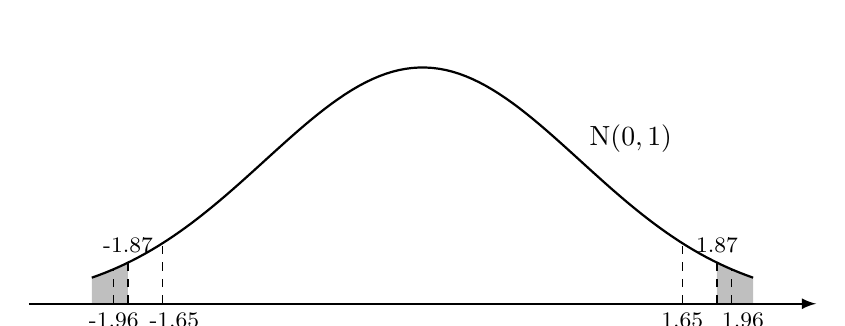
\begin{tikzpicture}[xscale=2, yscale=3]
			\fill[gray!50](-2.1, 0)--(-2.1, 0.11)--(-1.87, 0.174)--(-1.87,0);
			\fill[gray!50](2.1, 0)--(2.1, 0.11)--(1.87, 0.174)--(1.87,0);
			\draw[thick, -latex](-2.5, 0)--(2.5, 0);
			\draw[thick, domain=-2.1:2.1, samples=100]plot(\x,{exp(-\x*\x/2)});
			\node[above right]at(1, 0.6){$\Norm(0,1)$};
			\draw[dashed](1.65, 0)node[below]{\footnotesize 1.65}--(1.65, 0.256);
			\draw[dashed](1.87, 0)--(1.87, 0.174)node[above]{\footnotesize 1.87};
			\draw[dashed](1.96, 0)node[below]{\footnotesize\quad 1.96}--(1.96, 0.146);
			\draw[dashed](-1.65, 0)node[below]{\footnotesize\quad -1.65}--(-1.65, 0.256);
			\draw[dashed](-1.87, 0)--(-1.87, 0.174)node[above]{\footnotesize -1.87};
			\draw[dashed](-1.96, 0)node[below]{\footnotesize -1.96}--(-1.96, 0.146);
		\end{tikzpicture}
	\end{center}
\end{example}
\begin{definition}{检验$P$值}{}
	定义当$H_0$为真时,检验统计量的观测值以及更极端的观测出现的概率称为检验的$P$值。
\end{definition}
当$P$值$\leqslant\alpha$时拒绝$H_0$,也称为观测值显著。
\begin{compactenum}
	\item $P$值$=\P(\text{观测值及更极端的观测}|H_0)\neq\P(H_0|\text{观测值})$
	\item 若$P$值不小,则不拒绝$H_0$,原因可能为:(a) $H_0$为真;(b) $H_0$为假,但检验功效低。
\end{compactenum}
\begin{method}{$P$值检验法}{}
	\begin{compactenum}
		\item 提出假设$H_0,H_1$
		\item 给定$\alpha>0$
		\item 选择检验统计量,确定“极端”的形式(由$H_1$决定)
		\item 采样,计算检验统计量的值
		\item 计算$P$值
		\item 比较$P$值与$\alpha$,进行决策
	\end{compactenum}
\end{method}
\begin{example}{选举问题}{}
	$n=1200$,调查到的支持比例为
	\[
		\frac{684}{1200}\doteq 0.57=:p_n,
	\]
	考虑 
	\[
		H_0:p=p_0,\quad H_1:p>p_0.
	\]
	检验统计量$P_n$,由CLT
	\[
		\frac{P_n-p}{\sqrt{p(1-p)/n}}\dotsim\Norm(0,1)
	\]
	当$H_0$为真时,
	\[
		Z:=\frac{P_n-p_0}{se(P_0)}\dotsim\Norm(0,1),\quad se(P_n)=\sqrt{\frac{p_0(1-p_0)}n}.
	\]
	则$P$值
	\[
		\P_{p=p_0}(P_n\geqslant p_n)\doteq\P(Z\geqslant z_0),\quad z_0:=\frac{p_n-p_0}{se(P_n)}
	\]
	若$p_0=0.55$,则$P$值$=0.081$;若$p_0=0.5$,则$P$值$\ll 0.01$。
	\tcblower
	考虑复合假设 
	\[
		H_0:p\leqslant p_0,\quad H_1:p>p_0.
	\]
	可以取
	\[
		\hat{se}(P_n)=\sqrt{\frac{p_n(1-p_n)}n}=0.014
	\]
	当原假设为真时
	\[
		\P_{p\leqslant p_0}(P_n\geqslant p_n)\doteq\P_{p\leqslant p_0}\biggkh{Z\geqslant\frac{p_n-p}{\hat{se}(P_n)}}%\doteq 1-\Phi\biggkh{\frac{p_n-p}{\hat{se}(P_n)}},\quad p\leqslant p_0
	\]
	若拒绝$H_0:\theta\in\varTheta_0\ifnf T(X_1,\ldots,X_n)\geqslant c$,则
	\[
		\text{检验的}~P~\text{值}:=\sup_{\theta\in\varTheta_0}\P_{\theta}\Bigfkh{T(X_1,\ldots,X_n)\geqslant T(x_1,\ldots,x_n)}
	\]
	故
	\[
		P~\text{值}=\sup_{p\leqslant p_0}\P\biggkh{Z\geqslant\frac{p_n-p}{\hat{se}(P_n)}}=\P\biggkh{Z\geqslant\frac{p_n-p_0}{\hat{se}(P_n)}}.
	\]
	同$p=p_0$的情况。
\end{example}
\subsection{Bayes假设检验}
\begin{example}{}{Bayes test}
	掷10次硬币,观测到正面朝上$x$次
	\[
		H_0:p=0.5,\quad H_1:p=0.7,
	\]
	则
	\begin{align}\label{Bayes test}
		\frac{\P(H_0|x)}{\P(H_1|x)}=\frac{\P(H_0)\P(x|H_0)}{\P(H_1)\P(x|H_1)}<1\enspace(\text{或}\ll 1)
	\end{align}
	时拒绝$H_0$
\end{example}
若$H_0:\theta=\theta_0$,$\varTheta$连续,则$\P(H_0|x)=\P(\varTheta=\theta_0|x)\equiv 0$,此时需要技术性处理,可参考陈5.2.8
\paragraph{Review}
\begin{compactenum}
	\item Neyman-Pearson假设检验:临界值、$P$值检验法
		Bayes假设检验,主观解释概率,引入随机变量认知参数
	\item 临界值:拒绝域形状;$P$值:更极端形式
	%\item Pearson-$\chi^2$检验是一个多项分布的检验
\end{compactenum}
\subsection{拟合优度检验}
\begin{theorem}{$\chi^2$检验法}{chi2 test}
	设总体$X$的分布未知,检验假设
	\begin{align*}
		H_0&:\text{总体分布函数为}~F(x)\\
		H_1&:\text{总体分布函数不是}~F(x)
	\end{align*}
	将在$H_0$下$X$可能取值的全体$\Omega$分成互不相交的子集$A_1,\ldots,A_k$,$p_i:=\P(A_i)$。
	观测到样本值$x_1,\ldots,x_n$落在$A_i$的频数为$f_i$,相应的期望频数为$np_i$,Pearson证明:
	\begin{align}
		\chi^2:=\sum_{i=1}^k\frac{(f_i-np_i)^2}{np_i}\dotsim\chi^2(k-1).
	\end{align}
	拒绝域$\chi^2\geqslant\chi^2_\alpha(k-1).$
\end{theorem}
推导过程见 \href{https://en.wikipedia.org/wiki/Pearson%27s_chi-squared_test}{Pearson's chi-squared test}。应用中需要$n\geqslant 50,\enspace np_i\geqslant 5$,才能较好运用这个定理。
\begin{example}{均匀的骰子}{}
	\begin{center}
		\begin{tabular}{cccccccc}
			\toprule
			点数&1&2&3&4&5&6&total\\
			\midrule
			观测频数$f_i$&4&6&17&16&8&9&60\\
			\bottomrule
		\end{tabular}
	\end{center}
	检验假设
	\[
		H_0:\text{均匀}(p_1=p_2=\cdots=p_6),\quad H_1:\text{不均匀}
	\]
	Pearson $\chi^2$统计量的观测值
	\[
		\chi^2:=\sum_{i=1}^k\frac{(f_i-np_i)^2}{np_i}=14.2.
	\]
	检验$P$值$=\P_{H_0}(\chi^2(5)\geqslant\chi^2)=0.014$
\end{example}
连续情况,划分区间,分别计算参数$\theta$的MLE $\theta^\ast$,卡方统计量分布近似$\chi^2(k-1-r)$,其中$r=\dim(\theta)$。但分别计算MLE非常麻烦。

实践中先计算$\theta$的MLE $\theta^\ast$,再划分区间,计算$p_i$,卡方统计量分布不是近似$\chi^2(k-1-r)$,但是检验$P$值介于分布$\chi^2(k-1-r)$和$\chi^2(k-1)$算得的$P$值之间。

事实:独立的卡方统计量可以合并,自由度相应的相加。
\begin{example}{Mendel豌豆实验}{}
	Mendel的实验全部独立(不同作物组),Fisher计算其每个卡方统计量并且合并,得到的卡方统计量$\chi^2=41.6056$,自由度为84,$P$值
	\[
		\P(\chi^2(84)\geqslant\chi^2)=0.99993
	\]
	\textit{were far too perfect},Fisher对这个extraordinary result没有发表任何评论,只是指出\textit{the bias seems to pervade the whole of the data.}
\end{example}
\subsection{列联表检验}
列联表(conttingency table)是一种按两个属性作双向分类的表。
\begin{center}
	\tablechap{$a\times b$列联表}
	\begin{tabular}{c|ccc|c}
		\toprule
		&A$_1$&$\cdots$&A$_a$&total\\
		\hline
		B$_1$&$n_{11}$&$\cdots$&$n_{a1}$&$n_{\cdot 1}$\\
		$\vdots$&$\vdots$&$\ddots$&$\vdots$&$\vdots$\\
		B$_b$&$n_{1b}$&$\cdots$&$n_{ab}$&$n_{\cdot b}$\\
		\hline
		total&$n_{1\cdot}$&$\cdots$&$n_{a\cdot}$&$n$\\
		\bottomrule
	\end{tabular}
\end{center}
\begin{example}{独立性检验}{independent test}
	样本写在列联表中
	\[
		H_0:~\text{独立}~(p_{ij}=p_{i\cdot}p_{\cdot j})\quad H_1:~\text{不独立}
	\]
	在$H_0$为真的前提下,估计$p_{ij}$,MLE解得
	\[
		p_{ij}^\ast=p_{i\cdot}^\ast p_{\cdot j}^\ast=\frac{n_{i\cdot}}n\frac{n_{\cdot j}}n.
	\]
	卡方统计量
	\begin{align}
		\chi^2=\sum_{i=1}^a\sum_{j=1}^b\frac{(nn_{ij}-n_{i\cdot}n_{\cdot j})^2}{nn_{i\cdot}n_{\cdot j}}.
	\end{align}
	自由度$=ab-1-(a-1+b-1)=(a-1)(b-1)$。
	\tcblower
	特别的,当$a=b=2$时,自由度为1
	\[
		\chi^2=\frac{n(n_{11}n_{22}-n_{12}n_{21})^2}{n_{1\cdot}n_{2\cdot}n_{\cdot 1}n_{\cdot 2}}.
	\]
\end{example}
\begin{example}{齐性检验}{}
	Jane Austen作家,仿写
	\begin{center}
		\tablechap{Jane Austen作品单词频数\footnote{A: Sense and Sensibility. B: Emma. C: Sadition (unfinished). c: Sadition (imitation)}}
		\begin{tabular}{c|ccc|c|c}
			\toprule
			&A&B&C&total&c\\
			\hline
			a&147&186&101&434&83\\
			an&25&26&11&62&29\\
			this&32&39&15&86&15\\
			that&94&105&37&236&22\\
			with&59&74&28&161&43\\
			without&18&10&10&38&4\\
			\hline
			total&375&440&202&1017&196\\
			\bottomrule
		\end{tabular}
	\end{center}
	(1)检验Austen不同作品中单词用法的一致性
	\[
		H_0:~\text{具有一致性}~(p_{i1}=p_{i2}=p_{i3})
	\]
	在$H_0$为真的前提下,$p_1^\ast=434/1017$等,卡方统计量观测值
	\[
		\chi^2=12.27,
	\]
	自由度为10,$P$值$\sim 0.3$,故不拒绝$H_0$。

	(2)检验仿写者与Austen不同单词的用法的一致性
	\[
		H_0:~\text{具有一致性}~(p_{i\cdot}=p_{i\mathrm c})
	\]
	可得$\chi^2=32.81$,自由度5,$P$值$<10^{-3}$,拒绝$H_0$。
\end{example}
\subsection{似然比检验}
\begin{example}{}{}
	接例 \ref{exm:Bayes test},式(\ref{Bayes test})中,考虑
	\[
		\underset{\text{后验比}}{\frac{\P(H_0|x)}{\P(H_1|x)}}=\underset{\text{先验比}}{\frac{\P(H_0)}{\P(H_1)}}\underset{\text{似然比}}{\frac{\P(x|H_0)}{\P(x|H_1)}}<1\enspace(\text{或}\ll 1)
	\]
	时拒绝$H_0$;似然比检验就是当
	\[
		\frac{\P(x|H_0)}{\P(x|H_1)}\leqslant c
	\]
	时拒绝$H_0$。
\end{example}
可以证明,当$H_0,H_1$均为简单假设时,似然比检验是最优的。

当$H_0,H_1$不是简单假设时,
\[
	H_0:\theta\in\varTheta_0\quad H_1:\theta\in\varTheta_1
\]
得到随机样本$X_1,\ldots,X_n$,定义广义似然比
\[
	\Lambda^\ast:=\frac{\sup_{\theta\in\varTheta_0}L(\theta)}{\sup_{\theta\in\varTheta_1}L(\theta)}.
\]
基于技术原因,检验统计量为
\begin{align}
	\Lambda:=\frac{\sup_{\theta\in\varTheta_0}L(\theta)}{\sup_{\theta\in\varTheta_0\cup\varTheta_1}L(\theta)}\equiv\frac{\sup_{\theta\in\varTheta_0}L(\theta)}{L(\theta^\ast)}.
\end{align}
易得,当$\theta^\ast\in\varTheta_0$时,$\Lambda=1>\Lambda^\ast$,当$\theta^\ast\in\varTheta_1-\varTheta_0$时,$\Lambda=\Lambda^\ast$,即
\[
	\Lambda%(X_1,\ldots,X_n)
	=\min(\Lambda^\ast,1).
\]
$\Lambda$越小则样本越不支持$H_0$。
\begin{method}{临界值检验}{}
	选择$\lambda_0$使得$\P(\Lambda\leqslant\lambda_0|H_0)\leqslant\alpha$,若$H_0$为真时$\Lambda$的分布方便求,则可直接计算$\P(\Lambda\leqslant\lambda_0|H_0)$。
\end{method}
\begin{theorem}{}{}
	在一定光滑性的条件下,%当$n\to\infty$时,
	在$H_0$为真的前提下,
	\begin{align}
		-2\ln\Lambda\dto\chi^2(d).
	\end{align}
	其自由度$d=\dim(\varTheta_0\cup\varTheta_1)-\dim(\varTheta_0)$,$\dim$表示自由参数的个数。
\end{theorem}
\begin{example}{多项分布的似然比估计}{}
	多项分布
	\[
		H_0:p_1=p_1^0,\ldots,p_k=p_k^0,\enspace(p_1^0+\cdots+p_k^0=1)
	\]
	观测频数$n_1,\ldots,n_k$,$n_1+\cdots+n_k=n$,似然函数
	\[
		L(p_1,\ldots,p_k)={n\choose n_1,\ldots,n_k}p_1^{n_1}\cdots p_k^{n_k},
	\]
	故
	\[
		\Lambda=\frac{L(p_1^0,\ldots,p_k^0)}{L(p_1^\ast,\ldots,p_k^\ast)},\quad p_i^\ast=\frac{n_i}n.
	\]
	则
	\begin{align*}
		-2\ln\Lambda&=-2\sum_{i=1}^k n_i\ln\biggkh{\frac{p_i^0}{p_i^\ast}}=2\sum_{i=1}^kn_i\ln\biggkh{\frac{n_i}{np_i^0}}\\
		&=\cancel{2\sum_{i=1}^k(n_i-np_i^0)}+\sum_{i=1}^k\frac{(n_i-np_i^0)^2}{np_i^0}+\cdots
	\end{align*}
	$\dim(\varTheta_0)=0,\enspace\dim(\varTheta_0\cup\varTheta_1)=k-1$
\end{example}
\subsection{两总体的比较}
两独立总体$X,Y$比较,均值方差分别为$\mu_1,\mu_2,\sigma_1^2,\sigma_2^2$

\begin{example}{比较成功率}{}
	阿司匹林对于降低心脏病发病率的有效性(历时5年),样本信息:
	\begin{center}
		\tablechap{阿司匹林}
		\begin{tabular}{c|cccc}
			\toprule
			&心脏病发作&未发作&合计&发作率\\
			\midrule
			安慰剂&239&10795&11034&0.0217\\
			阿司匹林&129&10898&11037&0.0126\\
			\bottomrule
		\end{tabular}
	\end{center}
	安慰剂和阿司匹林组的发作率为$p_1,p_2$,假设检验 
	\[
		H_0:p_1=p_2\,(\text{无效}),\quad H_1:p_1>p_2\,(\text{有效})
	\]
	故
	\[
		\E(P_1-P_2)=p_1-p_2,\enspace\Var(P_1-P_2)=\frac{p_1(1-p_1)}{n_1}+\frac{p_2(1-p_2)}{n_2}.
	\]
	且
	\[
		\frac{(P_1-P_2)-(p_1-p_2)}{\hat{se}}\dotsim\Norm(0,1),
	\]
	在$H_0$为真的前提下,$p_1=p_2=:p$,
	\begin{align*}
		p^\ast=\frac{k_1+k_2}{n_1+n_2},\enspace\hat{se}=\sqrt{p^\ast(1-p^\ast)\biggkh{\frac1{n_1}+\frac1{n_2}}}=0.00175
	\end{align*}
	检验$P$值$=\P(Z\geqslant 5.20)\ll 10^{-3}$,拒绝$H_0$。
\end{example}
注:随机分组,双盲实验,$n$充分大。

\subsection{显著性思考}
假设检验不能解释原因,不能检验试验设计,实验者需要对样本负责。

统计显著$\neq$实际显著(陈P236)

\clearpage
\section{方差分析和回归分析}
\subsection{方差分析}
方差分析(Analysis of Variance, AoV or ANOVA)由著名英国统计学家R.A.Fisher在1923年提出,又称F检验,用于两个及两个以上样本均数差别的显著性检验。

我们要考察的指标称为试验指标。
影响试验指标的条件称为因素。
因素所处的状态称为因素的水平。

单因素试验:在一项试验中只有一个因素在改变,
多因素试验:多于一个因素在改变。

\paragraph{基本假设}
\begin{compactenum}
	\item 样本相互对立,来自正态总体
	\item 各总体方差相等
\end{compactenum}
\paragraph{变差分解}
组数$s$,总例数$N=\textstyle\sum_{j=1}^sn_j$

\begin{definition}{总变差}{total sum of square}
	总变差的大小可用总偏差平方和表示
	\begin{align}
		S_T:={}&\sum_{j=1}^s\sum_{i=1}^{n_j}(X_{ij}-\avg X)^2\\\notag
		={}&\sum_{i,j}X_{ij}^2-\frac1N\biggkh{\sum_{i,j}X_{ij}}^2,
	\end{align}
	反映了所有观测值之间总的变差程度。

	总自由度$\nu_T=N-1$,总均方$MS_T=S_T/\nu_T.$
\end{definition}
变异程度除与偏差平方和$S$有关外,还与其自由度$\nu$有关,由于各部分自由度不相等,因此各部分偏差平方和不能直接比较,须将各部分偏差平方和除以相应自由度,其比值称为均方差 ,简称均方(mean square, MS)。
\begin{definition}{组间变差}{error sum of square}
	各处理组的样本均值大小不等, 这种变差称为组间变差%,其大小可用各组均值$X_{\cdot j}$与总均值$X$的离均差平方和表示。记作$S_A$
	\begin{align}
		S_A:={}&\sum_{j=1}^sn_j(\avg X_{\cdot j}-\avg X)^2\\\notag
		={}&\sum_{j=1}^s\frac1{n_j}\biggkh{\sum_{i=1}^{n_j}X_{ij}}^2-\frac1N\biggkh{\sum_{i,j}X_{ij}}^2,
	\end{align}
	组间自由度$\nu_A=s-1$,组间均方$MS_A=S_A/\nu_A.$
\end{definition}
组间变差存在的原因
\begin{compactitem}
	\item 随机误差,包括个体变差和测量误差
	\item 处理因素的不同水平可能对实验结果有影响。
\end{compactitem}
\begin{definition}{组内变异}{treatment sum of square}
	在同一处理组内,虽然各受试对象接受的处理相同,但测量值之间仍不同,这种变异称为组内变异(误差)
	\begin{align}
		S_E:={}&\sum_{i,j}(X_{ij}-\avg X_{\cdot j})^2%\\\notag
		%={}&\sum_{j=1}^s(n_j-1)S_i^2.
	\end{align}
	反映了随机误差的影响。

	组内自由度$\nu_E=N-s$,组内均方$MS_E=S_E/\nu_E.$
\end{definition}
偏差平方和与自由度具有可加性
\begin{align*}
	S_T&=S_A+S_E,\\
	\nu_T&=\nu_A+\nu_E.
\end{align*}
假设检验
\[
	H_0:\mu_1=\mu_2=\cdots,\quad H_1:\ldots
\]
检验统计量 
\begin{align}
	F:=\frac{S_A}{S_E}\sim\mathrm F(\nu_A,\nu_E).
\end{align}
当$F>F_\alpha(\nu_A,\nu_E)$时拒绝$H_0$。
\paragraph{双因素检验}
设有两个因素$A,B$作用于试验的指标。因素$ A $有$ r $个水平$ A_1, A_2,\ldots, A_r$,因素$ B $有$ s $个水平$ B_1, B_2,\ldots, B_s $。现对因素$ A, B $的所有组合$(A_i, B_j)$都作$t$次试验,称为等重复试验。

设$X_{ijk}\sim\Norm(\mu_{ij},\sigma^2)$,$i, j, k $分别为因素$ A, B $和重复试验的下标。
则
总平均
\[
	\mu:=\frac1{rs}\sum_{i,j}\mu_{ij},
\]
$A_i,B_j$的效应分别为
\[
	\alpha_i=\mu_{i\cdot}-\mu,\quad\beta_j=\mu_{\cdot j}-\mu,
\]
交互效应
\[
	\gamma_{ij}=\mu_{ij}-\mu_{\cdot j}-\mu_{i\cdot}+\mu.
\]
可见
\[
	\sum_{i=1}^r\alpha_i=\sum_{i=1}^r\gamma_i,\quad\sum_{j=1}^s\beta_j=\sum_{j=1}^s\gamma_j.
\]
\begin{compactitem}
	\item $S_T$为总变差,自由度$rst-1$
	\item $S_E$误差平方和,自由度$rs(t-1)$
	\item $S_A,S_B$为因素$ A, B $的效应平方和,自由度为$ r - 1, s - 1$
	\item $S_{A\times B}$为$A,B$的交互效应平方和,自由度为 $(r - 1)(s - 1)$
\end{compactitem}
\begin{align}\notag
	S_T={}& \sum_{i=1}^r \sum_{j=1}^s \sum_{k=1}^t(X_{i j k}-\avg{X})^2 \\\notag
	={}& \sum_{i=1}^r \sum_{j=1}^s \sum_{k=1}^t[(X_{i j k}-\avg{X}_{i j \cdot})+(\avg{X}_{i\cdot\cdot}-\avg{X})+(\avg{X}_{\cdot j \cdot}-\avg{X})+\\\notag
	&\quad(\avg{X}_{i j \cdot}-\avg{X}_{i \cdot\cdot}-\avg{X}_{\cdot j \cdot}+\avg{X})]^2 \\\notag
	={}& \sum_{i=1}^r \sum_{j=1}^s \sum_{k=1}^t(X_{i j k}-\avg{X}_{i j \cdot})^2+s t \sum_{i=1}^r(\avg{X}_{i\cdot\cdot}-\avg{X})^2+ \\\notag
	& r t \sum_{j=1}^s(\avg{X}_{\cdot j \cdot}-\avg{X})^2+t \sum_{i=1}^r \sum_{j=1}^s(\avg{X}_{i j \cdot}-\avg{X}_{i\cdot\cdot}-\avg{X}_{\cdot j \cdot}+\avg{X})^2\\
	={}&S_E+S_A+S_B+S_{A\times B}.
\end{align}
比如,对A做假设检验
\[
	H_0:\alpha_1=\cdots=\alpha_r=0,\quad H_1:\ldots
\]
检验统计量 
\[
	F:=\dvd{\frac{S_A}{r-1}}{\frac{S_E}{rs(t-1)}}\sim\mathrm F\bigkh{r-1,rs(t-1)}.
\]

\subsection{回归分析}
%如果变量$x$和$y$从相关图中可以看出它们之间大致形成一种直线关系,我们就可在相关图上求出一条与各点最相配合的直线。一元线性回归方程$y=a+bx$

%设$(x_1,y_1),\ldots,(x_n,y_n) $是$ (x, y) $的一组观测值,对每个样本观测值$(x_i,y_i)$考虑与其回归值$a+bx_i$的离差为$y_i-a-bx_i$,离差平方和
用$g(X)$估计$Y$,离差$Y-g(X)$,均方误差就是离差平方的期望
\[
	Q:=\E\bigfkh{(Y-g(X))^2}.
\]
最小二乘法所求的是均方误差意义下的最优线性预测
\[
	(\alpha,\beta)=\arg\min_{a,b}\E\bigfkh{(Y-(a+bX))^2}
\]
实际上就是求二元函数
\begin{align*}
	f(a,b):=&{}\E\bigfkh{(Y-(a+bX))^2}\\
	=&{}\E(X^2)b^2+2\E(X)ab+a^2-2\E(XY)b-2\E(Y)a+\E(Y^2).
\end{align*}
的最小值点,则在最小值点处有
\[
	\pv fa=0,\enspace\pv fb=0.
\]
解得
\begin{align}
	\begin{cases}
		\beta=\frac{\E(XY)-\E(X)\E(Y)}{\E(X^2)-\E^2(X)}\equiv\frac{\Cov(X,Y)}{\Var(X)},\\
		\alpha=\E(Y)-\beta\E(X)
	\end{cases}
\end{align}
误差的期望和方差
\begin{align*}
	\E[Y-(\alpha+\beta X)]&=\E(Y)-\alpha-\beta\E(X)=0;\\
	\Var[Y-(\alpha+\beta X)]&=\Var(Y-\beta X)\\
	&=\Var(Y)+\beta^2\Var(X)-2\beta\Cov(Y,X)\\
	&=%\Var(Y)-\frac{\Cov^2(X,Y)}{\Var(X)}=
	\bigfkh{1-\Corr^2(X,Y)}\Var(Y).
\end{align*}
\paragraph{相关性检验}
对任意两个变量的一组观察值$ {(xi, yi)} $都可以用最小二乘法形式上求得$ y$对$ x $的回归方程,如果$ y $与$ x $没有线性相关关系, 这种形式的回归方程就没有意义。因此需要考察$ y $与$ x $间是否确有线性相关关系,这就是回归效果的检验问题。

一元线性回归模型
\[
	y=a+bx+\epsilon,\enspace\epsilon\sim\Norm(0,\sigma^2).
\]
因随机因素引起的误差称为残差平方和
\[
	Q_e=\sum_{i=1}^n(y_i-\hat y_i)^2
\]
则
\[
	\frac{Q_e}{\sigma^2}\sim\chi^2(n-2),\thus\hat\sigma^2=\frac{Q_e}{n-2},
\]
检验假设 
\[
	H_0:b=0,\quad H_1:b\neq 0,
\]
$\hat b$满足 
\[
	\hat b\sim\Norm\biggkh{b,\frac{\sigma^2}{L_{xx}}},\quad L_{xx}:=\sum_{i=1}^n(x_i-\avg x)^2.
\]
如果原假设成立,
\[
	\frac{\hat b\sqrt{L_{xx}}}{\sigma}\sim\Norm(0,1),\quad\frac{Q_e}{\sigma^2}\sim\chi^2(n-2).
\]
检验统计量 
\begin{align}
	t:=\hat b\sqrt{\frac{(n-2)L_{xx}}{Q_e}}\sim\mathrm t(n-2).
\end{align}
拒绝域$\abs t\geqslant t_{\alpha/2}(n-2).$
\paragraph{线性化回归}
在许多实际问题中,两个变量之间并不一定是线性关系,而是某种曲线关系,应该用曲线来拟合。可以进行适当的变量代换,把它线性化,这样就把一个非线性回归问题化为线性回归问题而得以解决。
\paragraph{多线性回归}
随机变量$ Y $往往与多个变量$ x1, x2, \ldots , xp $有关。对自变量$ x1, x2, \ldots, xp $的一组确定的值,$Y $有它的分布
\[
	Y=b_0+\sum_{i=1}^pb_ix_i+\epsilon,\enspace\epsilon\sim\Norm(0,\sigma^2).
\]

\clearpage
\section{随机抽样}
\subsection{Monte Carlo方法}
Monte Carlo方法是用随机数解决计算问题方法的统称。
\begin{theorem}{von Neumann舍选法}{}
	\begin{compactenum}
		\item 选取容易抽样的分布$h(x)$,使得曲线$Ch(x)$可以覆盖待抽样的分布$f(x)$;
		\item 从$h(x)$抽样得$x_i$;
		\item 从$\Unif(0,1)$抽样得$r_i$;
		\item 若$r_iCh(x_i)\leqslant f(x_i)$,则保留$x_i$,否则舍弃;
		\item 被接受的$x_i$序列,服从以$f(x)$为概率密度的分布;
		\item 使用$x_i$序列的算术平均,估算数学期望
	\end{compactenum}
\end{theorem}
第4步是舍选法的关键步骤,但在高维问题中,无法知道$f(x)$的绝对数值,只知道相对值。
\begin{theorem}{Markov链法}{}
	把$f(x_i)$与上一个采样点$f(x_{i-1})$比较,决定是否保留,以概率
	\[
		\min\biggfkh{1,\frac{f(x_i)}{f(x_{i-1})}}
	\]
	的概率接受$x_i$,否则令$x_i=x_{i-1}$。
\end{theorem}
\subsection{Bootstrap自助法}
\begin{quote}
	\textit{Why can not a man lift himself by pulling up on his bootstraps?}
\end{quote}
\begin{method}{bootstrap自助法}{}
	\begin{compactenum}
		\item 把样本看作总体的估计
		\item 从样本抽样
		\item 统计量
	\end{compactenum}
\end{method}
\begin{definition}{经验分布函数}{}
	$x_1,\ldots,x_n$是来自分布函数为$\CDF(x)$总体$X$的样本观察值。$X$的经验分布函数$\CDF_n(x)$定义为
	\begin{align}
		\CDF_n(x)=\frac1n\sum_{i=1}^nI(x\geqslant x_i).
	\end{align}
	用经验分布函数$\CDF_n$估计总体分布函数$\CDF$。
\end{definition}
从$\CDF_n$抽样可以看作是对样本$x_1,\ldots,x_n$进行可放回的重新抽样,称作bootstrap样本,记为$x_1^\ast,\ldots,$或$\bm x^\ast$。

使用一系列$\bm x^\ast$,得到相应的$\hat\theta_b^\ast=\hat\theta(\bm x_b^\ast)$。定义
\[
	\avg\theta^\ast=\frac1B\sum_{i=1}^B\hat\theta_b^\ast.
\]
为$\theta$的bootstrap估计。
\begin{theorem}{bootstrap中心极限定理}{bootstrap CLT}
	当总体$\CDF $换为经验分布$\CDF_n $时,$\E(\hat\theta)\to\avg\theta^\ast$,$\theta\to\hat\theta$
	\begin{align}
		\avg\theta^\ast-\hat\theta\pto\E(\hat\theta)-\theta.
	\end{align}
	收敛速度比正态分布CLT预测得更快,称为自助法的二次修正。
\end{theorem}
计算$\E_{\CDF_n}(\hat\theta)$需要考虑所有的$n^n$种重抽样可能性。计算量过大,改良为使用Monte Carlo方法近似从$ x_1, \ldots, x_n $进行随机重抽样
\clearpage
\section{随机过程}
随机过程的研究对象是随时间演变的随机现象。

不能用随机变量或多维随机变量来合理表达,而需要用一族 (无限多个) 随机变量来描述。
\begin{definition}{随机过程}{stochastic process}
	随机过程(stochastic process)是一族随机变量$\set{X(t)}{t\in T}$,其中$ t $是 参数,$T$称为参数集。
\end{definition}
对随机过程进行一次试验(即在$ T $上进行一次全程观测),其结果是$t$的函数,记作$\set{x(t)}{t\in T}$,称为随机过程的一个样本函数。

可将随机过程写成
\[
	\set{X(\omega,t)}{\omega\in\Omega,t\in T}
\]
的形式,其中$\omega,\Omega$分别是随机试验的样本点和样本空间。
\paragraph{统计学描述}~
\begin{definition}{一维分布函数}{}
	对随机过程$\set{X(t)}{t\in T}$,对每个固定的$t$
	\begin{align}
		\CDF_X(x,t):=\P\bigkh{X(t)\leqslant x},\enspace x\in\RR,
	\end{align}
	称为随机过程的一维分布函数,$\set{\CDF_X(x,t)}{t\in T}$称为一维分布函数族。
\end{definition}
类似地,可以推广定义$n$维分布函数(族)。有限维分布函数可以完全确定随机过程的统计特性。
\begin{definition}{随机过程的数字特征}{}
	均值函数$\mu_X(t):=\E\bigkh{X(t)}$,
	均方值函数$\Psi^2_X(t):=\E\bigkh{X^2(t)}$

	方差函数$\sigma_X^2(t):=\Var\bigkh{X(t)}$,
	标准差函数$\sigma_X(t):=\sqrt{\sigma^2_X(t)}$

	相关函数$R_X(s,t):=\E\bigkh{X(s)X(t)}$

	协方差函数$C_X(s,t):=\Cov\bigkh{X(s),X(t)}$
\end{definition}
不难得到
\begin{align*}
	\sigma_X^2(t)&=R_X(t,t)-\mu_X^2(t),\\
	C_X(s,t)&=R_X(s,t)-\mu_X(s)\mu_X(t).
\end{align*}
\subsection{独立增量过程}
\begin{definition}{独立增量过程}{}
	若$\forall t_1<\cdots<t_n(n\geqslant2, t_i\in T)$,诸增量
	\[
		X(t_2)-X(t_1),\ldots,X(t_n)-X(t_{n-1}),
	\]
	相互独立,则称$\set{X(t)}{t\in T}$是一个独立增量过程。
\end{definition}
\begin{theorem}{独立增量过程的性质}{}
	若$\set{X(t)}{t\in T}$是一个独立增量过程,且$X(0)=0$,则:
	\begin{compactitem}
		\item $X(t)$的有限维分布函数族可以由增量$X(t_2)-X(t_1)(t_2\geqslant t_1\geqslant 0)$的分布所确定
		\item 设$\sigma^2_X(t)$已知,则协方差函数
		\begin{align}
			C_X(s,t)=\sigma^2_X\bigkh{\min(s,t)}.
		\end{align}
	\end{compactitem}
\end{theorem}
\begin{definition}{Poisson过程}{}
	计数过程$\set{N(t)}{t\geqslant 0}$称为强度$\lambda>0$的时齐Poisson过程(homogeneous Poisson process),若满足:
	\begin{compactenum}
		\item $N(0)=0$
		\item $\set{N(t)}{t\geqslant 0}$是时齐的独立增量过程
		\item $\forall t>0,\D t>0$有
		\begin{compactitem}
			\item $\P\bigkh{N(t+\D t)-N(t)=1}=\lambda\D t+o(\D t)$
			\item $\P\bigkh{N(t+\D t)-N(t)\geqslant 2}=o(\D t)$
		\end{compactitem}
	\end{compactenum}
\end{definition}
Poisson过程中任意长度为$ t $的区间中事件个数$\sim\Pois(\lambda t).$
\begin{theorem}{Poisson过程的性质}{}
	%若$\set{N(t)}{t\geqslant 0}$是一个强度为$\lambda$的Poisson过程,则
	$N(t)\sim\Pois(\lambda t),\enspace\mu_N(t)=\lambda t,\enspace\sigma^2_N(t)=\lambda t,\enspace R_N(s,t)=\lambda\min(s,t).$%的一维分布是参数为$\lambda t$的Poisson分布。
\end{theorem}
\paragraph{二项分布视角}
将区间$ [0, t] $分为$ k $份,
当$k\to\infty$时,$N(t)\sim\Bern(k,p)$
\[
	\mu_N(t)=\lim_{k\to\infty}kp=\lim_{k\to\infty}k\biggfkh{\frac{\lambda t}k+o\biggkh{\frac tk}}=\lambda t+o(t).
\]
\paragraph{指数分布视角}
将Poisson过程第$ n $个事件发生时刻记为$ T_n$。记$\D T_n=T_n-T_{n-1} $为第$ n $个事件的等待时间,特别地$\D T_1 = T_1$。
\begin{theorem}{Poisson过程的指数间隔}{}
	$\D T_1,\D T_2,\ldots$ iid $\sim\Expo(\lambda)$
	\begin{align*}
		\P(\D T_1>t)&=\P\bigkh{N(t)=0}=\e{-\lambda t};\\
		\P(\D T_2>t|T_1=s)&=\P\bigkh{N(t+s)-N(t)=0\cancel{|T_1=s}}=\e{-\lambda t}.
	\end{align*}
	由全概率公式,$\P(\D T_2>t)=\E_{T_1}\bigfkh{\P(\D T_2>t|T_1)}=\e{-\lambda t}.$
\end{theorem}
\begin{theorem}{Poisson过程判定}{}
	给定iid随机变量列$\{\D T_i\sim\Expo(\lambda)\}$。称第$ n $个事件在时间$T_n =\D T_1 + \cdots +\D T_n $发生,得到$\set{N(t)=\max(n)}{t\geqslant T_n}$
	是强度为$\lambda$的时齐Poisson过程。
\end{theorem}
\begin{definition}{Wiener过程}{Wiener process}
	满足一下条件的随机过程$\set{W(t)}{t\geqslant 0}$称为Wiener过程若
	\begin{compactitem}
		\item $W(0)=0$
		\item $\set{W(t)}{t\geqslant 0}$是时齐的独立增量过程
		\item 增量服从正态分布,即$\forall t\geqslant s\geqslant 0$
		\[
			W(t)-W(s)\sim\Norm\bigkh{0,(t-s)\sigma^2}.
		\]
		若$\sigma=1$,则称为 标准Wiener过程。
	\end{compactitem}
\end{definition}
Brown运动是Wiener过程。
\begin{theorem}{Wiener过程的性质}{}
	$W(t)\sim\Norm(0,\sigma^2t),\enspace\mu_W(t)=0,\enspace\sigma^2_W(t)=\sigma^2t,\ldots$%,\enspace R_W(s,t)=\sigma^2\min(s,t)
\end{theorem}
任意Wiener过程$W(t)$,可令$W(t)/\sigma$转化为标准Wiener过程。

对$t_1<\cdots<t_n$,标准Wiener过程的各个增量
\begin{align*}
	W(t_1)&=w_1\sim\Norm(0,t_1),\\
	W(t_2)-W(t_1)&=w_2-w_1\sim\Norm(0,t_2-t_1),\\
	\vdots\\
	W(t_n)-W(t_{n-1})&=w_n-w_{n-1}\sim\Norm(0,t_n-t_{n-1}).
\end{align*}
独立,则$W(t_1),\ldots,W(t_n)$的联合PDF为 
\begin{align*}
	&f_W(w_1,\ldots,w_n;t_1,\ldots,t_n)\\
	&=\frac{\exp\bigg\{{-\dfrac12\biggfkh{\dfrac{w_1^2}{t_1}+\dfrac{(w_2-w_1)^2}{t_2-t_1}+\cdots+\dfrac{(w_n-w_{n-1})^2}{t_n-t_{n-1}}}\bigg\}}}{\sqrt{2\pi t_1(t_2-t_1)\cdots(t_n-t_{n-1})}}.
\end{align*}
\begin{example}{白噪声}{}
	设$\set{W(t)}{t\geqslant 0}$为标准Wiener过程,令$f$为区间$[a,b]$有连续导数的函数,定义随机积分
	\[
		\int_a^bf(t)\d W(t)=\lim_{n\to\infty}\sum_{i=1}^n f(t_{i-1})\bigkh{W(t_i)-W(t_{i-1})},
	\]
	其中$a=t_1<t_2<\cdots<t_n=b$是区间$[a,b]$的一个划分。%类似分部积分,
	有
	\[
		\int_a^bf(t)\d W(t)=f(b)W(b)-f(a)W(a)-\int_a^bW(t)\d f(t).
	\]
	$\set{\d W(t)}{t\geqslant 0}$称为白噪声,即一个时变函数$f$在白噪声的介质中传播导致输出$\textstyle\int f(t)\d W(t).$
\end{example}
\subsection{Markov过程}
\begin{definition}{Markov过程}{}
	随机过程$\set{X(t)}{t\in T}$为Markov过程若%其状态空间为$I$,$\forall n\geqslant 3,t_1,t_2,\ldots,t_$
	\begin{align*}
		&\P\bigkh{X(t_n)\leqslant x_n|X(t_1)=x_1,\ldots,X(t_{n-1})=x_{n-1}}\\
		={}&\P\bigkh{X(t_n)\leqslant x_n|X(t_{n-1})=x_{n-1}}
	\end{align*}
	时间和状态都离散Markov过程称为Markov链,记为:
	\[
		\set{X_n=X(n)}{n=0,1,2,\ldots}.
	\]
\end{definition}
\begin{definition}{转移概率}{}
	条件概率 
	\[
		\P(X_{t+n}=j|X_t=i)=:p_{ij}(t,t+n)
	\]
	称为Markov链在时间$t$处于状态$i$条件下,在时间$t+n$转移到状态$j$的转移概率。
\end{definition}
显然,
\[
	\sum_{j=1}^\infty p_{ij}(t,t+n)=1,\enspace\forall i.
\]
$n$步转移概率矩阵为
\begin{align}
	P(n)=\begin{bmatrix}
		p_{11}(t,t+n)&p_{12}(t,t+n)&\cdots\\
		p_{21}(t,t+n)&p_{22}(t,t+n)&\cdots\\
		\vdots&\vdots&\ddots
	\end{bmatrix}
\end{align}
每一行元素概率为1.
\begin{definition}{时齐Markov链}{}
	若Markov链是时齐的,即$p_{ij}(t,t+n)=p_{ij}(n)$与$t$无关,则概率转移矩阵为
	\begin{align*}
		P(n)=\begin{bmatrix}
			p_{11}(n)&p_{12}(n)&\cdots\\
			p_{21}(n)&p_{22}(n)&\cdots\\
			\vdots&\vdots&\ddots
		\end{bmatrix}
	\end{align*}
	一步转移概率矩阵$P(1)=:P.$
\end{definition}
\begin{theorem}{Chapman-Kolomogorov方程}{}
	时齐Markov链,有
	\begin{align*}
		p_{ij}(m+n)=\sum_{k=1}^\infty p_{ik}(m)p_{kj}(n),\quad i,j=1,2,\ldots
	\end{align*}
\end{theorem}
可以简写成矩阵形式
\[
	P(m+n)=P(m)P(n).
\]
自然,$P(n)=P^n$,时齐的Markov链的有限维分布由初始分布和一步转移概率完全确定。
\begin{definition}{遍历性和极限分布}{}
	若时齐Markov链的转移概率$p_{ij}(n)$存在极限
	\[
		\pi_j:=\lim_{n\to\infty}p_{ij}(n),
	\]
	则称该链具有遍历性,又若$\textstyle\sum_{j}\pi_j=1$,则称行向量
	\[
		\pi=[\pi_0,\pi_1,\ldots]
	\]
	为该链的极限分布。
\end{definition}
\begin{theorem}{遍历性的充分条件}{}
	若存在正整数$m$使得$\forall i,j\in I$有$p_{ij}(m)>0$,则此链具有遍历性,且极限分布是矩阵方程
	\begin{align}
		\pi=\pi P
	\end{align}
	满足$\pi_j>0,\textstyle\sum_j\pi=1$的唯一解。
\end{theorem}
满足上述条件的Markov链的极限分布是该链的平稳分布,即若将$\pi$作为初始分布,那么每一时刻该链的分布都是$\pi$。
\begin{example}{雨伞问题}{}
	我有2把雨伞用于往返于家和办公室之间。若我从学校出发回家的时候正在下雨,我就会带一把雨伞去学校。从家去学校同理。假定我出发时下雨的概率是$ p$ (不依赖于过去)。

	令$ X(t) $为我所在地雨伞的数量,状态空间为$\{0, 1, 2\}$。
	
	一步转移概率矩阵
	\[
		P=\begin{bmatrix}
			0&0&1\\
			0&1-p&p\\
			1-p&p&0
		\end{bmatrix}
	\]
	$P_{ij}(4)>0$,故具有遍历性。极限分布
	\[
		\biggfkh{\frac{1-p}{3-p},\frac1{3-p},\frac1{3-p}}
	\]
	我被淋湿这件事等价于“处于状态0并且下雨”,即
	\[
		p\cdot\frac{1-p}{3-p}
	\]
\end{example}
\begin{example}{赌徒(续)}{gambler 2}
	在例 \ref{exm:gambler} 中,我们用全概率公式解决了赌徒问题,下面我们用Markov链解决,我们可以写出一步转移矩阵
	\[
		\begin{bmatrix}
			1&0&\cdots\\
			q&0&p&\cdots\\
			&q&0&p&\cdots\\
			&&q&0&\cdots\\
			&&&\ddots&\ddots\\
			&&&&\cdots&0&p\\
			&&&&\cdots&0&1
		\end{bmatrix}
	\]
	解得$P_i$,显然现实中$p$均$<1/2$,则当$N\to\infty$时,$P_i\equiv 0$,因此若不收手,终将破产。
\end{example}
\subsection{平稳随机过程}
随机过程作为“随机的函数”太一般了,太难了。如果给它加一些限制,可以使它更有用。迄今有三类限制在随机过程的研究中取得了突破,加深了我们对随机过程的理解
\begin{compactitem}
	\item Markov过程
	\item 鞅(martingales)
	
	未来给现有已知状态的增量期望为0。与stochastic calculus联系紧密,在博弈论和金融中使用。
	\item 平稳随机过程(stationary stochastic process)
	
	变量一般指时间,当变量为空间时为homogeneous stochastic process。
\end{compactitem}
\begin{definition}{严平稳过程}{}
	统计性质不随机时间变化的随机过程,即
	\begin{align*}
		\CDF_X(t_1,\ldots,t_n)=\CDF_X(t_1+\tau,\ldots,t_n+\tau)
	\end{align*}
	称为严平稳随机过程,简称严平稳过程。
\end{definition}
一个平稳的Gauss过程同时也是严平稳的,因为Gauss过程的有限分布函数由一二阶矩完全确定。
\begin{definition}{平稳过程}{}
	一二阶矩不随机时间变化的随机过程,即
	\begin{align}
		\mu_X(t)=\mu_X,\quad R_X(t,t+\tau)=R_X(\tau)
	\end{align}
	那么该随机过程称为宽平稳过程(weak stationary stochastic process),广义平稳过程或平稳过程。
\end{definition}
独立增量过程与平稳过程无关,至少从二阶矩的角度,
\[
	R_X(t,t+\tau)=\sigma^2_X(t)+\mu_X(t)\mu_X(t+\tau)
\]
与$t$相关。易证,
Poisson过程和Wiener过程都不是平稳过程。

但是它们的均值与自方差函数对时间平移的导数都是常数,
可以通过微分或差分转化成平稳随机过程,称为广义(差分)平稳随机过程。
\paragraph{相关函数}
平稳过程的均值函数为常数,因此相关函数$R_X(\tau)$包含了平稳过程的主要信息。但相关函数$R_X(\tau)$并不能完整刻画随机过程的所有统计学性质。
\begin{theorem}{平稳随机过程的性质}{}
	\begin{compactitem}
		\item $R_X(\tau)$是偶函数,且在0处取最大值
		\item 若$\exists\tau\neq 0,|R_X(\tau)|=R_X(0)$,则$X(t)$是周期的
		\item 若$R_X(\tau)$在0处连续,则处处连续
		\item $R_X(\tau)$非负定,即$\forall t_i\in T,g(t)$
		\[
			\sum_{i,j=1}^nR_X(t_i-t_j)g(t_i)g(t_j)\geqslant 0.
		\]
		任意连续的非负定函数都是某平稳过程的自相关函数。
	\end{compactitem}
\end{theorem}
标准自协方差函数
\[
	\rho_X(\tau)=\frac{C_X(\tau)}{C_X(0)}.
\]
特别地,当$\mu_X(t)\equiv 0$时,
\[
	\rho_X(\tau)=\frac{R_X(\tau)}{R_X(0)}.
\]
\begin{example}{随机相位正弦波}{}
	随机过程$X(t)=A\cos(\omega t+\theta)$
\end{example}
对于随机相位正弦波$\{X(t)\}$,$R_X(0)=\E\bigkh{X^2(t)}$具有功率的意义。
\begin{compactitem}
	\item 多个随机相位正弦波叠加的信号,总功率为各个分量功率之和。
	\item 借助Fourier分解推广,可定义功率谱函数$S_X(\omega)$,其加和为$R_X(0)$,与$R_X(\tau)$互为Fourier变换。
\end{compactitem}

\paragraph{遍历性与估计}
均值函数
\[
	\mu_X(t):=\E\bigkh{X(t)}
\]
定义为随机过程的期望,称为系综平均。
\begin{compactitem}
	\item 如果事件能在系综里假想发生,那么它就一定会在一次足够长的观测中发生。(Landau统计力学)
	\item 系综平均$\mu_X(t)$指在假想的多个随机过程的样本轨迹下,$t $时刻观测值的平均。
	\item 对于平稳过程,如果观测足够长时间,是否可以与多个样本轨迹等价?即平稳过程相距较大的观测值$ X(t) $与$ X(t + \tau) $之间,是否可看作不相关?
\end{compactitem}
\begin{definition}{时间均值}{}
	记$x_1:=x(t_1)$,定义时间均值为
	\[
		\hat m_n:=\frac{x_1+\cdots+x_n}n\to m
	\]
\end{definition}
若
\[
	\sum_{\tau=0}^\infty R_X(\tau)<\infty
\]
那么
\[
	\hat m_n\pto\mu_X.
\]
此时称过程$ X(t) $的均值具有各态历经
性(ergodicity)或遍历性。
\begin{compactitem}
	\item $\hat m_n$是$\mu_X$的无偏相合估计量。
	\item 估计量的方差\[
		\lim_{n\to\infty}n\Var(\hat m_n)=\sum_{\tau=-\infty}^{+\infty}R_X(\tau)
	\]
\end{compactitem}
区间估计:如果相关性较弱,适用CLT,可使用正态近似给出区间估计。

自相关函数的估计
\[
	\hat R_n(\tau)=\frac1n\sum_{t=1}^{n-\tau}(x_t-\hat m)(x_{t+\tau}-\hat m).
\]
\subsection{时间序列}
时间序列是离散平稳过程的特例,与滤波理论联系紧密。
\begin{definition}{平稳时间序列}{}
	若时间序列$\{X_t\}$是平稳过程,称之为平稳时间序列。
	\[
		\E(X_t)=\mu,\quad\E(X_tX_{t+\tau})=f(\tau).
	\]
	定义
	\[
		\gamma_k:=\E\bigfkh{(X_t-\mu)(X_{t+k}-\mu)}=f(\tau)-\mu^2
	\]
	是平稳过程的协方差函数$R_X(\tau)$的离散版本。
\end{definition}
与$R_X(\tau)$性质类似,$\gamma_k$偶函数、非负定、$\gamma_0$最大,定义自相关函数
\[
	\rho_k:=\frac{\gamma_k}{\gamma_0}.
\]
\begin{definition}{偏相关函数}{}
	用$X_t$的前$ k $个时刻的值$X_{t-1},\ldots,X_{t-k}$对$ X_t $做最小二乘估计,即
	\[
		a_{k1},\ldots,a_{kk}=\arg\min\E\biggfkh{\biggkh{X_t-\sum_{i=1}^ka_{ki}X_{t-i}}^2}
	\]
	其中$a_{kk}$称作$X_t$的偏相关函数。
\end{definition}
$k\geqslant 3$,偏相关函数值变得不显著。
\subsubsection{AR(\textit{p})模型}
\begin{definition}{白噪声序列}{}
	时间序列$\{\epsilon_t\}$是白噪声序列若
	\[
		\E(\epsilon_t)=0,\quad\E(\epsilon_s\epsilon_t)=\sigma^2\delta_{st}.
	\]
	$\gamma_k=\sigma^2\delta_k$
\end{definition}
一般还可以再假设$\epsilon_t\sim\Norm(0,\sigma^2)$为Gauss白噪声序列。
\begin{definition}{AR($p$)过程}{}
	平稳过程$\{X_t\}$被叫作p阶自回归(auto-regression)过程,简记为AR($p$)过程,如果
	\begin{align}
		X_t-\varphi_1X_{t-1}-\cdots-\varphi_pX_{t-p}=\epsilon_t.
	\end{align}
	白噪声$\epsilon_t$是AR过程的创新(innovation)。
\end{definition}
在Gauss过程中,创新也是Gauss的。取名innovation代表给随机过程带来新的熵。
\begin{definition}{生成多项式}{}
	记延迟算子$ B $为
	\[
		BX_t=X_{t-1}
	\]
	则AR($p$)过程的条件可记为$\Phi(B)X_t=\epsilon_t$,其中
	\begin{align}
		\Phi(B)=1-\varphi_1B-\cdots-\varphi_pB^p
	\end{align}
	称为AR($p$)过程的生成多项式。
\end{definition}
只有$X_t$与$\epsilon_t$相关,即
\begin{align*}
	\Cov(\epsilon_t,X_s)=\begin{cases}
		0,&t>s\\[-1ex]
		\sigma^2,&t=s\\[-1ex]
		<\sigma^2,&t<s
	\end{cases}
\end{align*}
\begin{theorem}{AR($p$)的性质}{}
	\begin{compactitem}
		\item 生成多项式为$\Phi(\cdot)$的AR($p$)过程的功率谱为
		\[
			S_X(\omega)=\frac{\sigma^2}{|\Phi(\e{-\i\omega})|^2}.
		\]
		因此它的自相关函数$\gamma_k$作为$ S_X(\omega) $的Fourier变换,有无穷多非零项,称为拖尾的。
		\item 由AR($p$)的定义知,当$ k > p $时,它们偏相关函数$ a_{kk} = 0$,称为截尾的。
	\end{compactitem}
\end{theorem}
由于$\epsilon_t$是白噪声,即作为误差独立同分布,可以使用多线性回归模型来估计生成多项式中的系数$\varphi_1,\ldots,\varphi_p$
\[
	X_t=\varphi_1X_{t-1}+\cdots+\varphi_pX_{t-p}+\epsilon_t,\enspace\epsilon_t\sim\Norm(0,\sigma^2).
\]
\subsubsection{ARMA(\textit{p, q})}
\begin{definition}{ARMA($p,q$)}{}
	随机过程
	\[
		X_t=\epsilon_t-\theta_1\epsilon_{t-1}-\cdots-\theta_q\epsilon_{t-q}
	\]
	是有创新$\{\epsilon_t\}$和生成多项式
	\begin{align}
		\Theta(B)=1-\theta_1B-\cdots-\theta_qB^q
	\end{align}
	的滑动平均(moving-average)过程MA($q$)。
\end{definition}

\clearpage
\section{测量不确定度}
\begin{definition}{测量的术语}{terminology of measurement}
	\begin{compactitem}
		\item 误差(error) =测量值$-$参考值
		\item 不确定度(uncertainty):根据所用到的信息,表征赋予被测量量值分散性的非负参数。
		\item 系统误差(systematic error):在重复测量中保持不变或按可预见方式变化的测量误差的分量。
		
		参考值是(约定)真值,
		\item 随机误差(random error):在重复测量中按不可预见方式变化的测量误差的分量。
		
		系统误差=误差$-$随机误差
		\item A类评定(type A evaluation):对在规定测量条件下测得的量值用统计分析的方法进行测量不确定度分量的评定。
		\item B类评定:用不同于测量不确定度 A 类评定的方法对测量不确定度分量的评定。
		\item 合成标准不确定度:由在一个测量模型中各输入量的标准测量不确定度获得输出量的标准测量不确	定度。
	\end{compactitem}
\end{definition}
\paragraph{不确定度的传递}
一个被测量$ y $可能是通过对一些输入变量$x_1,\ldots,x_n$的测量而间接得到的。如果被测量$ y $和输入变量之间满足关系式
\[
	y=f(x_1,\ldots,x_n)
\]
则$ y $的标准不确定度$ u(y) $可以由输入变量的标准不确定度$u(x_1),\ldots,u(x_n)$通过下式计算得到:
\begin{align}
	u^2(y)=\sum_{i=1}^n\biggkh{\pv y{x_i}}^2u^2(x_i)
\end{align}
要求$x_i$之间互不相关。输入变量的标准不确定度可以是A类,也可以是B类。

若具有相关性,$\rho(x_i,x_j)\neq 0$
\begin{align}
	u^2(y)=\sum_{i,j}\rho(x_i,x_j)\pv y{x_i}\pv y{x_j}u(x_i)u(x_j).
\end{align}
\paragraph{扩展不确定度}
样本均值$\avg x$的置信区间
\[
	\biggkh{\mu\pm t_{\alpha}(\nu)\frac s{\sqrt n}}
\]
$\alpha$为置信度,$\nu$为自由度。$k=t_{\alpha}(\nu)$是置信因子。把一个估计值的标准差乘以$ k $便得到这个估计值在特定置信度下(一般95\%)的扩展不确定度。
\paragraph{不确定度的不确定度}
样本方差更一般的定义
\[
	s^2=\frac1\nu\sum_{i=1}^n\epsilon_i^2
\]
其中$\nu$为自由度,$\epsilon_i$为残差。

$s^2$常用作不确定度的A类估计,它自身的不确定度由$\chi^2$分布估计
\begin{align}\label{eqn:uncertainty of uncertainty}
	\frac\nu{\sigma^2}s^2\sim\chi^2(\nu),\thus u^2(s^2)=\frac{2\sigma^4}\nu.\tag{*}
\end{align}
如果$ s $表示测量值的标准不确定度,那么$ s $自身的不确定度$ u(s) $为
\[
	u^2(s)=\frac1{(2s)^2}u^2(s^2),\thus u(s)=\frac1{\sqrt{2\nu}}\frac{\sigma^2}s\doteq\frac s{\sqrt{2\nu}}.
\]
自由度$\nu$等于测量值的个数$ n $减去用这些测量值所决定的特征量的
个数。$s $的相对不确定度表示为
\[
	\frac{u(s)}s\sim\frac1{\sqrt{2\nu}}.
\]
如果$\nu<4$,那么$ s $的相对不确定度高达35\%;而如果$\nu>50$,那么$ s $的相对不确定度会降到$<10\%$。
\begin{theorem}{Welch-Satterthwaite公式}{}
	设两个互不相关的输入变量$x_1,x_2$,且输出变量$y=f(x_1,x_2)$,则有
	\[
		u^2(y)=c_1^2u^2(x_1)+c_2^2u^2(x_2),
	\]
	$y $对应的不确定度的不确定度为
	\[
		u^2\bigkh{u^2(y)}=c_1^4u^2\bigkh{u^2(x_1)}+c_2^4u^2\bigkh{u^2(x_2)},
	\]
	由$\chi^2$分布,利用“不确定度的不确定度”和自由度$\nu$的关系式(\ref{eqn:uncertainty of uncertainty})
	\[
		\frac{2u^4(y)}{\nu_{\mathrm{eff}}}=\frac{2c_1^4u^4(x_1)}{\nu_1}+\frac{2c_2^4u^4(x_2)}{\nu_2}.
	\]
	$\nu_{\mathrm{eff}}$为$ y $的等效自由度(不必为整数),则
	\[
		\frac{[c_1^2u^2(x_1)+c_2^2u^2(x_2)]^2}{\nu_{\mathrm{eff}}}=\frac{c_1^4u^4(x_1)}{\nu_1}+\frac{c_2^4u^4(x_2)}{\nu_2}.
	\]
\end{theorem}

\iffalse
\begin{compactenum}
	\item 
\end{compactenum}
\begin{compactitem}
	\item 
\end{compactitem}
\fi
\printindex
\end{document}